% Options for packages loaded elsewhere
\PassOptionsToPackage{unicode}{hyperref}
\PassOptionsToPackage{hyphens}{url}
%
\documentclass[
]{article}
\usepackage{amsmath,amssymb}
\usepackage{lmodern}
\usepackage{iftex}
\ifPDFTeX
  \usepackage[T1]{fontenc}
  \usepackage[utf8]{inputenc}
  \usepackage{textcomp} % provide euro and other symbols
\else % if luatex or xetex
  \usepackage{unicode-math}
  \defaultfontfeatures{Scale=MatchLowercase}
  \defaultfontfeatures[\rmfamily]{Ligatures=TeX,Scale=1}
\fi
% Use upquote if available, for straight quotes in verbatim environments
\IfFileExists{upquote.sty}{\usepackage{upquote}}{}
\IfFileExists{microtype.sty}{% use microtype if available
  \usepackage[]{microtype}
  \UseMicrotypeSet[protrusion]{basicmath} % disable protrusion for tt fonts
}{}
\makeatletter
\@ifundefined{KOMAClassName}{% if non-KOMA class
  \IfFileExists{parskip.sty}{%
    \usepackage{parskip}
  }{% else
    \setlength{\parindent}{0pt}
    \setlength{\parskip}{6pt plus 2pt minus 1pt}}
}{% if KOMA class
  \KOMAoptions{parskip=half}}
\makeatother
\usepackage{xcolor}
\usepackage[margin=1in]{geometry}
\usepackage{color}
\usepackage{fancyvrb}
\newcommand{\VerbBar}{|}
\newcommand{\VERB}{\Verb[commandchars=\\\{\}]}
\DefineVerbatimEnvironment{Highlighting}{Verbatim}{commandchars=\\\{\}}
% Add ',fontsize=\small' for more characters per line
\usepackage{framed}
\definecolor{shadecolor}{RGB}{248,248,248}
\newenvironment{Shaded}{\begin{snugshade}}{\end{snugshade}}
\newcommand{\AlertTok}[1]{\textcolor[rgb]{0.94,0.16,0.16}{#1}}
\newcommand{\AnnotationTok}[1]{\textcolor[rgb]{0.56,0.35,0.01}{\textbf{\textit{#1}}}}
\newcommand{\AttributeTok}[1]{\textcolor[rgb]{0.77,0.63,0.00}{#1}}
\newcommand{\BaseNTok}[1]{\textcolor[rgb]{0.00,0.00,0.81}{#1}}
\newcommand{\BuiltInTok}[1]{#1}
\newcommand{\CharTok}[1]{\textcolor[rgb]{0.31,0.60,0.02}{#1}}
\newcommand{\CommentTok}[1]{\textcolor[rgb]{0.56,0.35,0.01}{\textit{#1}}}
\newcommand{\CommentVarTok}[1]{\textcolor[rgb]{0.56,0.35,0.01}{\textbf{\textit{#1}}}}
\newcommand{\ConstantTok}[1]{\textcolor[rgb]{0.00,0.00,0.00}{#1}}
\newcommand{\ControlFlowTok}[1]{\textcolor[rgb]{0.13,0.29,0.53}{\textbf{#1}}}
\newcommand{\DataTypeTok}[1]{\textcolor[rgb]{0.13,0.29,0.53}{#1}}
\newcommand{\DecValTok}[1]{\textcolor[rgb]{0.00,0.00,0.81}{#1}}
\newcommand{\DocumentationTok}[1]{\textcolor[rgb]{0.56,0.35,0.01}{\textbf{\textit{#1}}}}
\newcommand{\ErrorTok}[1]{\textcolor[rgb]{0.64,0.00,0.00}{\textbf{#1}}}
\newcommand{\ExtensionTok}[1]{#1}
\newcommand{\FloatTok}[1]{\textcolor[rgb]{0.00,0.00,0.81}{#1}}
\newcommand{\FunctionTok}[1]{\textcolor[rgb]{0.00,0.00,0.00}{#1}}
\newcommand{\ImportTok}[1]{#1}
\newcommand{\InformationTok}[1]{\textcolor[rgb]{0.56,0.35,0.01}{\textbf{\textit{#1}}}}
\newcommand{\KeywordTok}[1]{\textcolor[rgb]{0.13,0.29,0.53}{\textbf{#1}}}
\newcommand{\NormalTok}[1]{#1}
\newcommand{\OperatorTok}[1]{\textcolor[rgb]{0.81,0.36,0.00}{\textbf{#1}}}
\newcommand{\OtherTok}[1]{\textcolor[rgb]{0.56,0.35,0.01}{#1}}
\newcommand{\PreprocessorTok}[1]{\textcolor[rgb]{0.56,0.35,0.01}{\textit{#1}}}
\newcommand{\RegionMarkerTok}[1]{#1}
\newcommand{\SpecialCharTok}[1]{\textcolor[rgb]{0.00,0.00,0.00}{#1}}
\newcommand{\SpecialStringTok}[1]{\textcolor[rgb]{0.31,0.60,0.02}{#1}}
\newcommand{\StringTok}[1]{\textcolor[rgb]{0.31,0.60,0.02}{#1}}
\newcommand{\VariableTok}[1]{\textcolor[rgb]{0.00,0.00,0.00}{#1}}
\newcommand{\VerbatimStringTok}[1]{\textcolor[rgb]{0.31,0.60,0.02}{#1}}
\newcommand{\WarningTok}[1]{\textcolor[rgb]{0.56,0.35,0.01}{\textbf{\textit{#1}}}}
\usepackage{longtable,booktabs,array}
\usepackage{calc} % for calculating minipage widths
% Correct order of tables after \paragraph or \subparagraph
\usepackage{etoolbox}
\makeatletter
\patchcmd\longtable{\par}{\if@noskipsec\mbox{}\fi\par}{}{}
\makeatother
% Allow footnotes in longtable head/foot
\IfFileExists{footnotehyper.sty}{\usepackage{footnotehyper}}{\usepackage{footnote}}
\makesavenoteenv{longtable}
\usepackage{graphicx}
\makeatletter
\def\maxwidth{\ifdim\Gin@nat@width>\linewidth\linewidth\else\Gin@nat@width\fi}
\def\maxheight{\ifdim\Gin@nat@height>\textheight\textheight\else\Gin@nat@height\fi}
\makeatother
% Scale images if necessary, so that they will not overflow the page
% margins by default, and it is still possible to overwrite the defaults
% using explicit options in \includegraphics[width, height, ...]{}
\setkeys{Gin}{width=\maxwidth,height=\maxheight,keepaspectratio}
% Set default figure placement to htbp
\makeatletter
\def\fps@figure{htbp}
\makeatother
\setlength{\emergencystretch}{3em} % prevent overfull lines
\providecommand{\tightlist}{%
  \setlength{\itemsep}{0pt}\setlength{\parskip}{0pt}}
\setcounter{secnumdepth}{5}
\usepackage{titling}

\pretitle{%
  \begin{center}
  \LARGE
  
\includegraphics[width=2cm,height=3cm]{ibama.png}\\[\bigskipamount]
}
\posttitle{\end{center}}
\ifLuaTeX
  \usepackage{selnolig}  % disable illegal ligatures
\fi
\IfFileExists{bookmark.sty}{\usepackage{bookmark}}{\usepackage{hyperref}}
\IfFileExists{xurl.sty}{\usepackage{xurl}}{} % add URL line breaks if available
\urlstyle{same} % disable monospaced font for URLs
\hypersetup{
  pdftitle={Introdução à Análise de Dados com Linguagem R},
  pdfauthor={Ambiental Robson Cruz},
  hidelinks,
  pdfcreator={LaTeX via pandoc}}

\title{Introdução à Análise de Dados com Linguagem R}
\usepackage{etoolbox}
\makeatletter
\providecommand{\subtitle}[1]{% add subtitle to \maketitle
  \apptocmd{\@title}{\par {\large #1 \par}}{}{}
}
\makeatother
\subtitle{Módulo 1}
\author{\nAnalista Ambiental Robson Cruz}
\date{}

\begin{document}
\maketitle

{
\setcounter{tocdepth}{2}
\tableofcontents
}
\hypertarget{introduuxe7uxe3o}{%
\section{Introdução}\label{introduuxe7uxe3o}}

R é uma linguagem de programação gratuita de código aberto usada
principalmente para computação estatística e gráficos. R é uma linguagem
interpretada semelhante a Python, onde você não precisa compilar
primeiro para executar seu programa. Depois de criar seu programa, você
pode executá-lo em uma ampla variedade de plataformas UNIX, Windows e
MacOS.

R é uma linguagem específica de domínio de código aberto, explicitamente
projetada para ciência de dados. Muito popular em finanças e academia, R
é uma linguagem perfeita para manipulação, processamento e visualização
de dados, bem como computação estatística e aprendizado de máquina.

Como qualquer outra linguagem de programação, R também suporta extensão
na forma de pacotes, portanto, os desenvolvedores podem criar seus
próprios pacotes e reutilizá-los quando necessário.

\hypertarget{instalauxe7uxe3o-do-r}{%
\section{Instalação do R}\label{instalauxe7uxe3o-do-r}}

A instalação padrão da linguagem R é feita a partir do CRAN, uma rede
formada de servidores espalhadod pelo mundo que armazena versões
atualizadas do código fonte e executável (Windows), assim como a
documentação da linguagem R.

\hypertarget{instalauxe7uxe3o-do-rstudio}{%
\section{Instalação do RStudio}\label{instalauxe7uxe3o-do-rstudio}}

RStudio é um ambiente de desenvolvimento integrado para linguagem R (IDE
- integrated development environment), porém pode rodar scripts SQL, C,
C++ e Python. A vantagem se se poder trabalhar com IDE é que ela
disponibiliza ferramentas de apoio ao desenvolvimento de códigos em
linguagem de programção. Para download do RStudio acesse o endereço
\url{https://www.rstudio.com/}, e escolha a opção RStudio Desktop

\hypertarget{conhecendo-a-interface-gruxe1fica-do-rstudio}{%
\subsection{Conhecendo a Interface Gráfica do
RStudio}\label{conhecendo-a-interface-gruxe1fica-do-rstudio}}

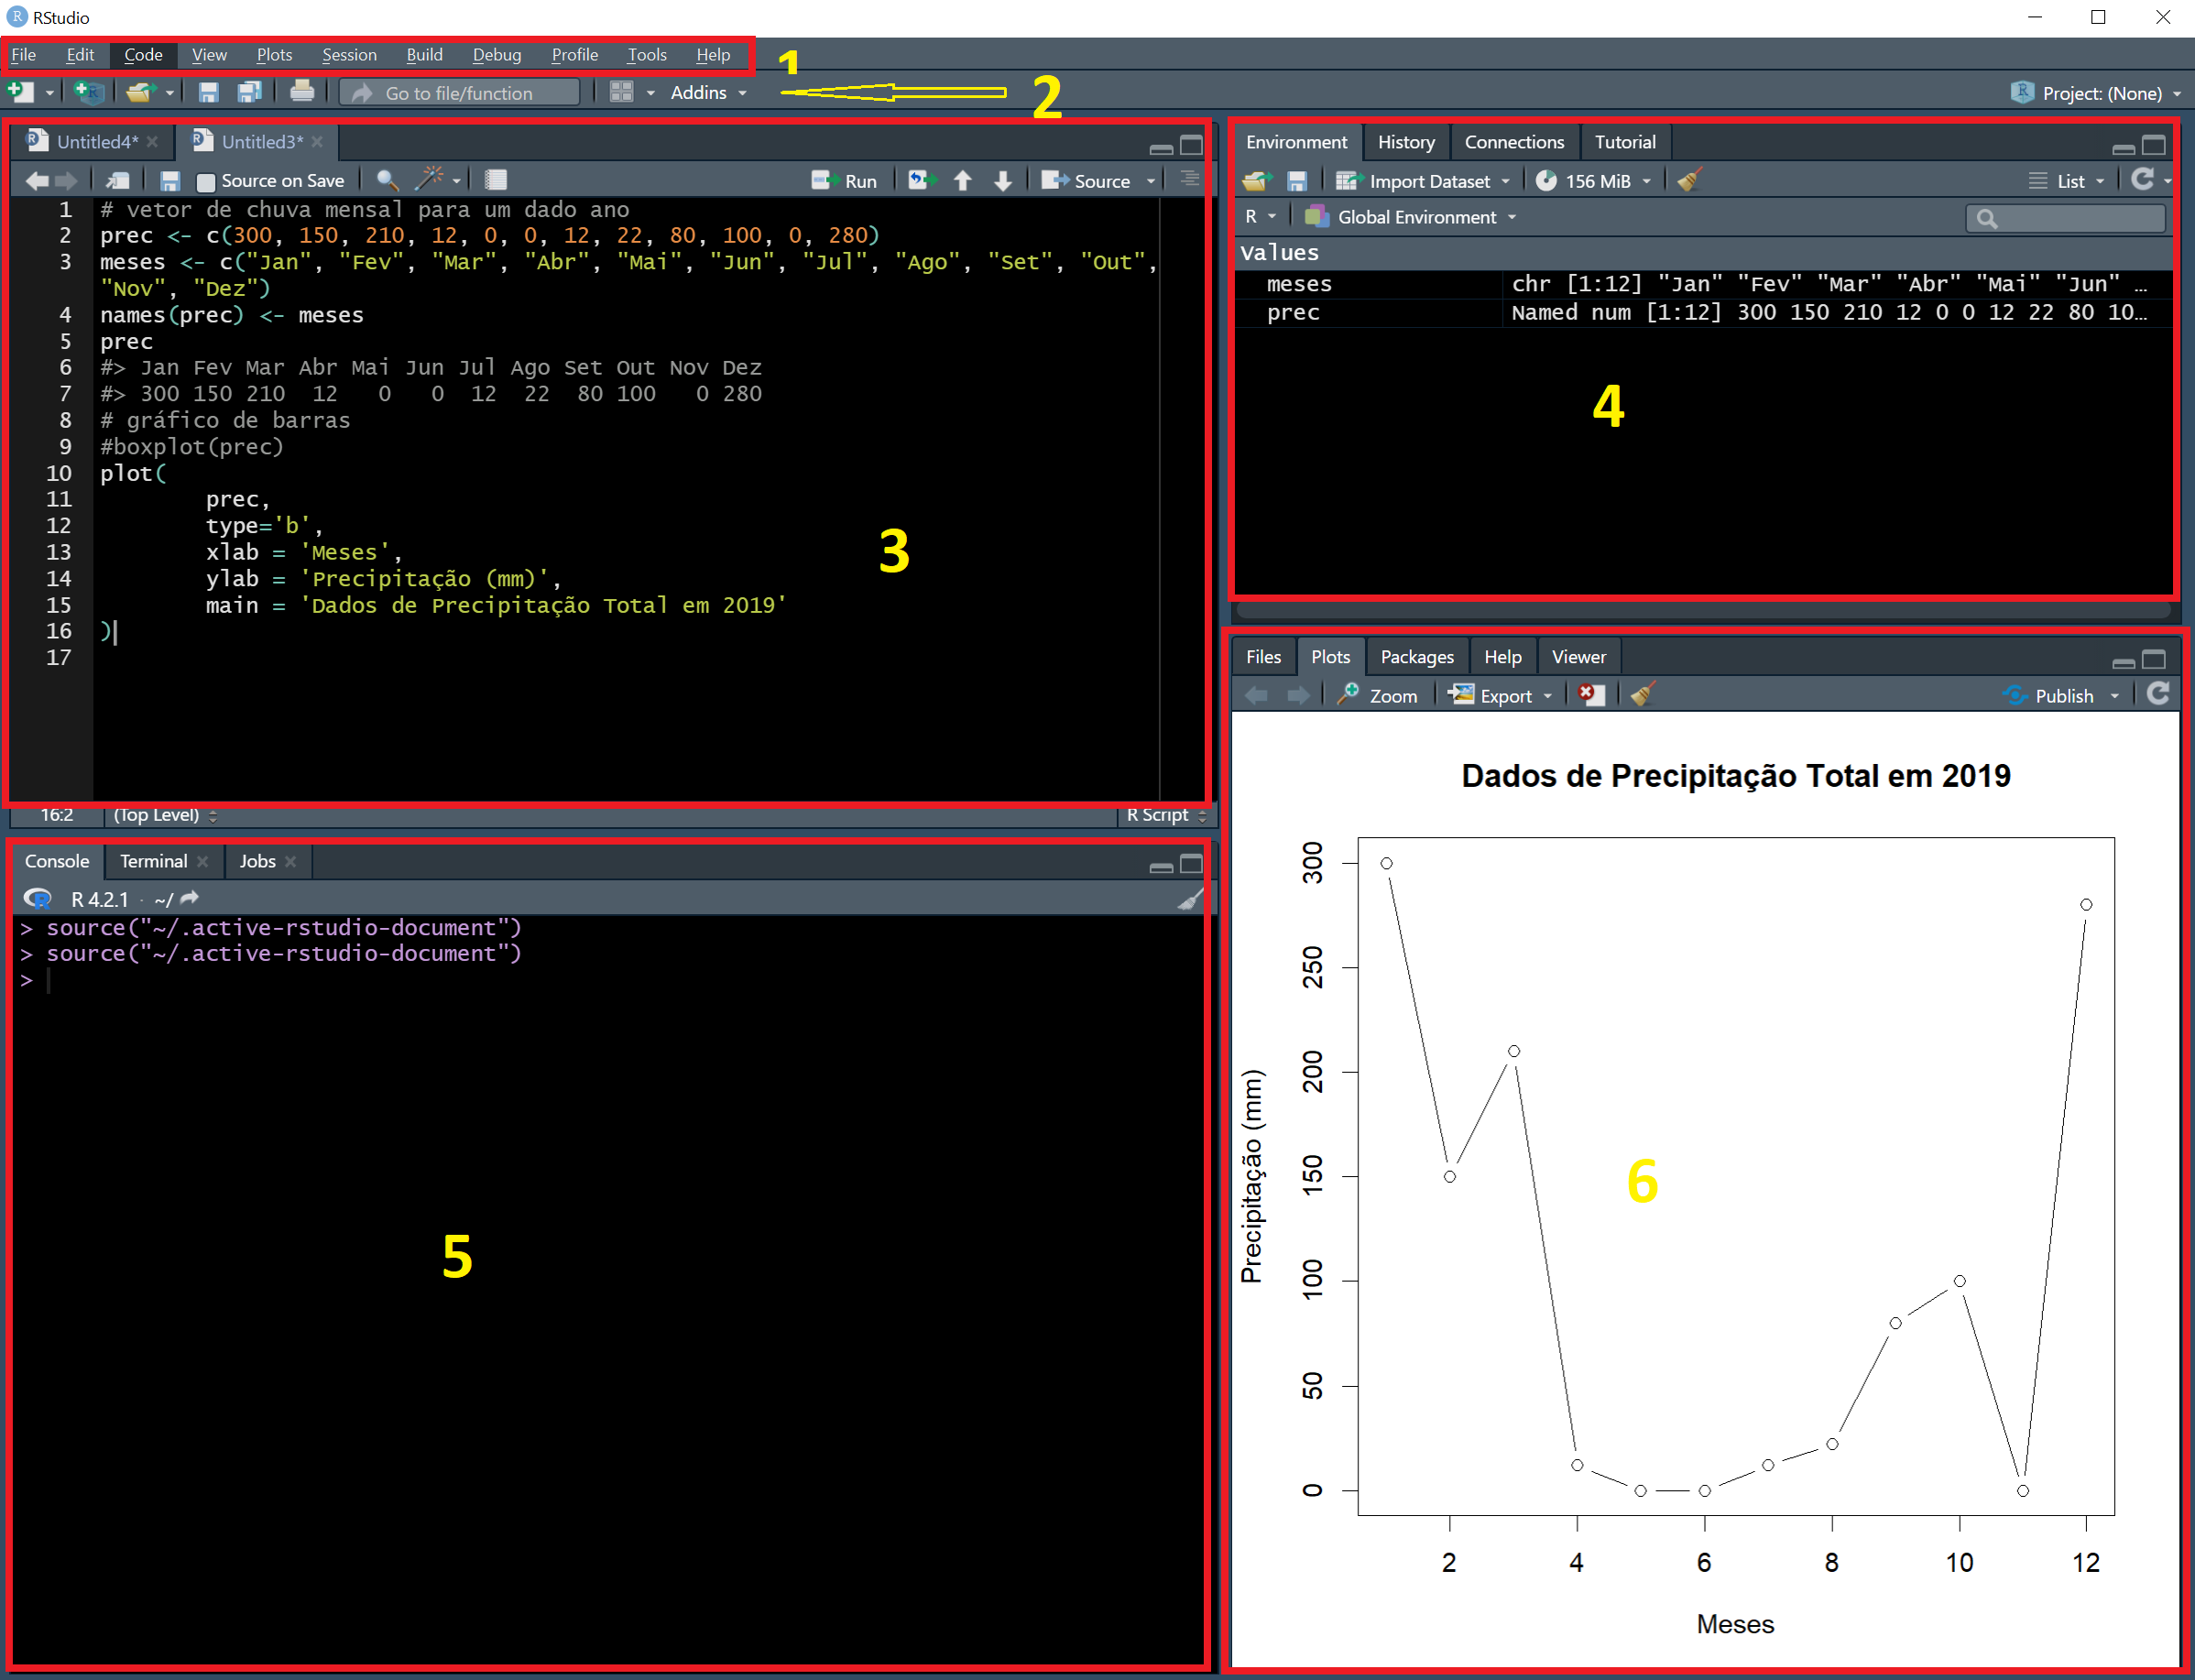
\includegraphics{./output/RStudio.PNG}

A interface do RStudio é divida em 4 painés, e duas barras: * 1 - Barra
de \emph{menu} * 2 - Barra de ferramentas * 3 - Painel de \emph{scripts}
e arquivos * 4 - Painel de variáveis de
Ambiente/Histórico/Conexões/Tutorial * 5 - Painel de
\emph{Console/Terminal} * 6 - Painel de Árvore de
Arquivos/Gráficos/Pacotes/Ajuda/Visualizador

\hypertarget{obter-e-configurar-o-ambiente-de-trabalho}{%
\subsection{Obter e Configurar o ambiente de
trabalho}\label{obter-e-configurar-o-ambiente-de-trabalho}}

Para obter o ambiente de trabalho atualmente em uso pelo RStudio
utilizamos a função getwd(); esta função vem do termo em inglês: Get
Working Directory, traduzido para o portugês como ``Obter Ambiente de
Trabalho''. No sistema operacional Windows, por padrão, o RStudio
configura o ambiente de trabalho em
``C:/Usuários/Nome\_do\_Usuário/Documentos''

.

Para configurar um ambiente de trabalho diferente do padrão utilizamos a
função setwd(). Esta função tem nome bem sugestivo na lingua inglesa, a
saber: Set Working Directory, ``Configurar Ambiente de Trabalho''.

\begin{Shaded}
\begin{Highlighting}[]

\end{Highlighting}
\end{Shaded}

\hypertarget{exercuxedcio-pruxe1tico---ambiente-de-trabalho}{%
\subsubsection{Exercício Prático - Ambiente de
trabalho}\label{exercuxedcio-pruxe1tico---ambiente-de-trabalho}}

\textbf{Instrução 1/2} * Use a janela console do RStudio para obter o
atual diretório de trabalho em uso no seu computador.

\begin{Shaded}
\begin{Highlighting}[]

\end{Highlighting}
\end{Shaded}

\textbf{Instrução 2/2} * Configure seu ambiente de trabalho para
\texttt{\textquotesingle{}C:/Users/Seu\_nome\_de\_usario/Downloads\textquotesingle{}}

\emph{Atenção: Em seu nome\_de\_usuario insira seu nome de usuário.}

\begin{Shaded}
\begin{Highlighting}[]

\end{Highlighting}
\end{Shaded}

\begin{Shaded}
\begin{Highlighting}[]

\end{Highlighting}
\end{Shaded}

\hypertarget{operadores-aritmuxe9ticos-e-de-atribuiuxe7uxe3o-em-r}{%
\section{Operadores Aritméticos e de Atribuição em
R}\label{operadores-aritmuxe9ticos-e-de-atribuiuxe7uxe3o-em-r}}

\begin{longtable}[]{@{}cc@{}}
\toprule()
Operador & Função \\
\midrule()
\endhead
+ & Soma \\
- & Subtração \\
/ & Divisão \\
* & Multiplicação \\
\%\% & Resto da divisão \\
\%/\% & Parte inteira divisão \\
\^{} & Potenciação \\
** & Potenciação \\
\textless- & Atribuição \\
= & Atribuição \\
\bottomrule()
\end{longtable}

\hypertarget{exercuxedcio-pruxe1tico---operadores-aritmuxe9ticos-e-de-atribuiuxe7uxe3o}{%
\subsection{Exercício Prático - Operadores Aritméticos e de
Atribuição}\label{exercuxedcio-pruxe1tico---operadores-aritmuxe9ticos-e-de-atribuiuxe7uxe3o}}

\textbf{Instrução 1/3} * Obter o resto da divisão entre os números
inteiros 10 e 3.

\begin{Shaded}
\begin{Highlighting}[]

\end{Highlighting}
\end{Shaded}

\textbf{Instrução 2/3} * Obter a parte interira da divisão de 10 por 3.

\begin{Shaded}
\begin{Highlighting}[]

\end{Highlighting}
\end{Shaded}

\textbf{Instrução 3/3} * Obter o quadrado de um número inteiro qualquer.

\begin{Shaded}
\begin{Highlighting}[]

\end{Highlighting}
\end{Shaded}

\hypertarget{operadores-de-comparauxe7uxe3o-em-r}{%
\section{Operadores de Comparação em
R}\label{operadores-de-comparauxe7uxe3o-em-r}}

\begin{longtable}[]{@{}cc@{}}
\toprule()
Operador & Significado \\
\midrule()
\endhead
== & igual a \\
!= & diferente de \\
\textgreater{} & maior que \\
\textless{} & menor que \\
\textgreater= & maior ou igual a \\
\textless= & menor ou igual a \\
\bottomrule()
\end{longtable}

\hypertarget{objeto-em-r}{%
\section{Objeto em R}\label{objeto-em-r}}

Um objeto é simplesmente qualquer variável que armaneza um caractere
numérico, alfabético ou uma cadeia de carateres (\emph{string}). Em R
temos objetos especiais para manipulação de grande volume de dados, a
exemplo de vetores, listas e dataframes. Para criação de um objeto se
utiliza o operador de atribuição \texttt{\textless{}-}. Nos exemplos a
seguir são criados os objetos \texttt{x}, \texttt{y} e \texttt{z} para
armazenar um número inteiro, uma letra e uma frase.

\begin{Shaded}
\begin{Highlighting}[]
\CommentTok{\# definição de um objeto do tipo inteiro}
\NormalTok{int }\OtherTok{\textless{}{-}} \DecValTok{42}

\CommentTok{\# definição de um objeto do tipo caractere}
\NormalTok{letra }\OtherTok{\textless{}{-}} \StringTok{"R"}

\CommentTok{\# \# definição de um objeto do tipo string (cadeia de caracteres)}
\NormalTok{string }\OtherTok{\textless{}{-}} \StringTok{"R é massa"}
\end{Highlighting}
\end{Shaded}

Em ambos os trechos de código acima se observa o uso do caractere
\texttt{\#}, em R e python este caractere é utilizado para fazer
comentário no código, portanto, toda linha que contém este caractere é
ignorada na execução do programa.

A seguir é mostrado como fazer comentário com várias linhas.

\begin{Shaded}
\begin{Highlighting}[]
\StringTok{"}
\StringTok{Este é um comentário em R utilizando }
\StringTok{várias linhas para documentação de}
\StringTok{códigos.}
\StringTok{"}
\end{Highlighting}
\end{Shaded}

\begin{verbatim}
## [1] "\nEste é um comentário em R utilizando \nvárias linhas para documentação de\ncódigos.\n"
\end{verbatim}

\hypertarget{conferindo-o-contuxe9udo-de-um-objeto}{%
\subsection{Conferindo o contéudo de um
objeto}\label{conferindo-o-contuxe9udo-de-um-objeto}}

Para conferir o conteúdo de um objeto em R, fazemos uma chamada
diretamento pelo nome do objeto de interesse ou através do uso da função
\emph{\texttt{print()}}

\begin{Shaded}
\begin{Highlighting}[]
\NormalTok{int}
\end{Highlighting}
\end{Shaded}

\begin{verbatim}
## [1] 42
\end{verbatim}

\begin{Shaded}
\begin{Highlighting}[]
\FunctionTok{print}\NormalTok{(int)}
\end{Highlighting}
\end{Shaded}

\begin{verbatim}
## [1] 42
\end{verbatim}

\begin{Shaded}
\begin{Highlighting}[]
\FunctionTok{cat}\NormalTok{(int)}
\end{Highlighting}
\end{Shaded}

\begin{verbatim}
## 42
\end{verbatim}

42

\hypertarget{descobrindo-o-tipo-de-dados-armazenado-em-um-objeto-r}{%
\subsection{Descobrindo o tipo de dados armazenado em um objeto
R}\label{descobrindo-o-tipo-de-dados-armazenado-em-um-objeto-r}}

Para descobrir o tipo de dados armazenado em um objeto, podemos utilizar
a função \emph{\texttt{class}}

\begin{Shaded}
\begin{Highlighting}[]
\FunctionTok{class}\NormalTok{(int)}
\end{Highlighting}
\end{Shaded}

\begin{verbatim}
## [1] "numeric"
\end{verbatim}

\begin{Shaded}
\begin{Highlighting}[]
\FunctionTok{class}\NormalTok{(letra)}
\end{Highlighting}
\end{Shaded}

\begin{verbatim}
## [1] "character"
\end{verbatim}

\begin{Shaded}
\begin{Highlighting}[]
\FunctionTok{class}\NormalTok{(string)}
\end{Highlighting}
\end{Shaded}

\begin{verbatim}
## [1] "character"
\end{verbatim}

\hypertarget{estrutura-de-dados-em-r}{%
\section{Estrutura de Dados em R}\label{estrutura-de-dados-em-r}}

\hypertarget{vetores}{%
\subsection{Vetores}\label{vetores}}

Vetor em R é um objeto R que armazena um ou mais elementos de valores
indexados, ou seja, cada elemento dentro do vetor possui uma posição
específica. Para criação de um vetor basta colocar os valores dentro de
\texttt{c()}. Vetor é uma estrutura de dados especialmente importante em
análise de dados. A seguir temos um exemplo de como criar um vetor de
inteiros.

\begin{Shaded}
\begin{Highlighting}[]
\NormalTok{inteiros }\OtherTok{\textless{}{-}} \FunctionTok{c}\NormalTok{(}\DecValTok{42}\NormalTok{, }\DecValTok{33}\NormalTok{, }\DecValTok{0}\NormalTok{, }\SpecialCharTok{{-}}\DecValTok{1}\NormalTok{, }\DecValTok{5}\NormalTok{)}
\end{Highlighting}
\end{Shaded}

Para acessar o primeiro elemento do vetor \texttt{inteiros} usamos o
comando \emph{\texttt{vetor{[}x{]}}}, onde \emph{vetor} é nome atribuido
ao vetor e \emph{x} é o índice do elemento a ser buscado no vetor. Se
quisermos mostrar apenas o elemento de índice 1 do vetor
\texttt{inteiros}, ou seja: filtar apenas o primeiro elemento, basta
usar \emph{\texttt{inteiros{[}1{]}}}

\begin{Shaded}
\begin{Highlighting}[]
\CommentTok{\# acessar o primeiro elemento de um vetor}
\NormalTok{inteiros[}\DecValTok{1}\NormalTok{]}
\end{Highlighting}
\end{Shaded}

\begin{verbatim}
## [1] 42
\end{verbatim}

Ao usar um índice negativo para filtrar um vetor estamos pedindo que a
saída dos daos do vetor não mostre o elemte relativo ao índice negativo.
No código a seguir vamos mostrar todos os elementos do vetor
\texttt{inteiros}, exceto o quarto elemento (elemento de índice 4).

\begin{Shaded}
\begin{Highlighting}[]
\CommentTok{\# mostrar todos os elementos do vetor com exeção do elemento de índice 4}
\NormalTok{inteiros[}\SpecialCharTok{{-}}\DecValTok{4}\NormalTok{]}
\end{Highlighting}
\end{Shaded}

\begin{verbatim}
## [1] 42 33  0  5
\end{verbatim}

\hypertarget{substituiuxe7uxe3o-de-elementos-de-um-vetor}{%
\subsubsection{Substituição de elementos de um
vetor}\label{substituiuxe7uxe3o-de-elementos-de-um-vetor}}

\begin{Shaded}
\begin{Highlighting}[]
\CommentTok{\# Substituir o primeiro elemento do vetor "inteiros" por 2}
\NormalTok{inteiros[}\DecValTok{1}\NormalTok{] }\OtherTok{\textless{}{-}} \DecValTok{2}
\NormalTok{inteiros}
\end{Highlighting}
\end{Shaded}

\begin{verbatim}
## [1]  2 33  0 -1  5
\end{verbatim}

\hypertarget{funuxe7uxf5es-buxe1sicas-aplicadas-a-vetores}{%
\subsubsection{Funções básicas aplicadas a
vetores}\label{funuxe7uxf5es-buxe1sicas-aplicadas-a-vetores}}

\begin{itemize}
\tightlist
\item
  \emph{\texttt{length()}} Retorna o tamanho de um vetor, ou seja, o
  número de elementos armazenados no vetor.
\end{itemize}

\begin{Shaded}
\begin{Highlighting}[]
\FunctionTok{length}\NormalTok{(inteiros)}
\end{Highlighting}
\end{Shaded}

\begin{verbatim}
## [1] 5
\end{verbatim}

\hypertarget{names-retorna-os-nomes-atribuuxeddos-a-cada-elemento-de-um-vetor}{%
\paragraph{\texorpdfstring{\emph{\texttt{names()}} Retorna os nomes
atribuídos a cada elemento de um
vetor}{names() Retorna os nomes atribuídos a cada elemento de um vetor}}\label{names-retorna-os-nomes-atribuuxeddos-a-cada-elemento-de-um-vetor}}

\begin{Shaded}
\begin{Highlighting}[]
\CommentTok{\# Defini um vetor de números inteiros chamado "dias\_semana"}
\NormalTok{dias\_semana }\OtherTok{\textless{}{-}} \FunctionTok{c}\NormalTok{(}\DecValTok{1}\SpecialCharTok{:}\DecValTok{7}\NormalTok{)}

\CommentTok{\# Mostrar na tela do console os dados do vetor}
\NormalTok{dias\_semana}
\end{Highlighting}
\end{Shaded}

\begin{verbatim}
## [1] 1 2 3 4 5 6 7
\end{verbatim}

\begin{Shaded}
\begin{Highlighting}[]
\CommentTok{\# Checar se o vetor possui nomes associados aos seus elementos}
\FunctionTok{names}\NormalTok{(dias\_semana)}
\end{Highlighting}
\end{Shaded}

\begin{verbatim}
## NULL
\end{verbatim}

\begin{Shaded}
\begin{Highlighting}[]
\CommentTok{\# Atribuir nomes aos elementos do vetor utilizando a função names()}
\FunctionTok{names}\NormalTok{(dias\_semana) }\OtherTok{\textless{}{-}} \FunctionTok{c}\NormalTok{(}\StringTok{\textquotesingle{}Domingo\textquotesingle{}}\NormalTok{, }\StringTok{\textquotesingle{}Segunda\textquotesingle{}}\NormalTok{, }\StringTok{\textquotesingle{}Terça\textquotesingle{}}\NormalTok{, }\StringTok{\textquotesingle{}Quarta\textquotesingle{}}\NormalTok{,}
                        \StringTok{\textquotesingle{}Quinta\textquotesingle{}}\NormalTok{, }\StringTok{\textquotesingle{}Sexta\textquotesingle{}}\NormalTok{, }\StringTok{\textquotesingle{}Sábado\textquotesingle{}}\NormalTok{)}
\end{Highlighting}
\end{Shaded}

\begin{Shaded}
\begin{Highlighting}[]
\CommentTok{\# Checar se o vetor possui nomes associados aos seus elementos}
\FunctionTok{names}\NormalTok{(dias\_semana)}
\end{Highlighting}
\end{Shaded}

\begin{verbatim}
## [1] "Domingo" "Segunda" "Terça"   "Quarta"  "Quinta"  "Sexta"   "Sábado"
\end{verbatim}

\begin{Shaded}
\begin{Highlighting}[]
\CommentTok{\# Mostrar na tela do console os dados do vetor}
\NormalTok{dias\_semana}
\end{Highlighting}
\end{Shaded}

\begin{verbatim}
## Domingo Segunda   Terça  Quarta  Quinta   Sexta  Sábado 
##       1       2       3       4       5       6       7
\end{verbatim}

\hypertarget{attributes-retorna-uma-lista-com-os-atributos-associados-a-um-vetor.}{%
\paragraph{\texorpdfstring{\emph{\texttt{attributes()}} Retorna uma
lista com os atributos associados a um
vetor.}{attributes() Retorna uma lista com os atributos associados a um vetor.}}\label{attributes-retorna-uma-lista-com-os-atributos-associados-a-um-vetor.}}

\begin{Shaded}
\begin{Highlighting}[]
\CommentTok{\# Verificar se os vetores "inteiros" e "dias\_semana"}
\CommentTok{\# possuem algum atributo}
\FunctionTok{attributes}\NormalTok{(inteiros)}
\end{Highlighting}
\end{Shaded}

\begin{verbatim}
## NULL
\end{verbatim}

\begin{Shaded}
\begin{Highlighting}[]
\FunctionTok{attributes}\NormalTok{(dias\_semana)}
\end{Highlighting}
\end{Shaded}

\begin{verbatim}
## $names
## [1] "Domingo" "Segunda" "Terça"   "Quarta"  "Quinta"  "Sexta"   "Sábado"
\end{verbatim}

\hypertarget{seq-cria-uma-sequuxeancia-dentro-de-um-vetor}{%
\paragraph{\texorpdfstring{\emph{\texttt{seq()}} Cria uma sequência
dentro de um
vetor}{seq() Cria uma sequência dentro de um vetor}}\label{seq-cria-uma-sequuxeancia-dentro-de-um-vetor}}

\begin{Shaded}
\begin{Highlighting}[]
\CommentTok{\# gerar uma sequência de 1 a 10, saltando 2 números}
\NormalTok{sequencia }\OtherTok{\textless{}{-}} \FunctionTok{seq}\NormalTok{(}\DecValTok{0}\NormalTok{, }\DecValTok{10}\NormalTok{, }\DecValTok{2}\NormalTok{)}
\FunctionTok{print}\NormalTok{(sequencia)}
\end{Highlighting}
\end{Shaded}

\begin{verbatim}
## [1]  0  2  4  6  8 10
\end{verbatim}

\hypertarget{rep-cria-uma-repetiuxe7uxe3o-de-um-vetor}{%
\paragraph{\texorpdfstring{\emph{\texttt{rep()}} Cria uma repetição de
um
vetor}{rep() Cria uma repetição de um vetor}}\label{rep-cria-uma-repetiuxe7uxe3o-de-um-vetor}}

\begin{Shaded}
\begin{Highlighting}[]
\CommentTok{\# Gerar uma repetição de três vezes o vetor formado pelos número de 1 a 4}
\FunctionTok{rep}\NormalTok{(}\DecValTok{1}\SpecialCharTok{:}\DecValTok{4}\NormalTok{, }\DecValTok{3}\NormalTok{)}
\end{Highlighting}
\end{Shaded}

\begin{verbatim}
##  [1] 1 2 3 4 1 2 3 4 1 2 3 4
\end{verbatim}

\hypertarget{duplicated-mostra-a-localizauxe7uxe3o-de-elementos-duplicados.}{%
\paragraph{\texorpdfstring{\texttt{duplicated()} Mostra a localização de
elementos
duplicados.}{duplicated() Mostra a localização de elementos duplicados.}}\label{duplicated-mostra-a-localizauxe7uxe3o-de-elementos-duplicados.}}

\begin{Shaded}
\begin{Highlighting}[]
\CommentTok{\# Vetor com números inteiros duplicados}
\NormalTok{vetor }\OtherTok{\textless{}{-}} \FunctionTok{c}\NormalTok{(}\DecValTok{1}\NormalTok{, }\DecValTok{2}\NormalTok{, }\DecValTok{1}\NormalTok{, }\DecValTok{3}\NormalTok{, }\DecValTok{4}\NormalTok{, }\DecValTok{5}\NormalTok{, }\DecValTok{4}\NormalTok{)}

\CommentTok{\# Mostrar os números duplicados}
\FunctionTok{duplicated}\NormalTok{(vetor)}
\end{Highlighting}
\end{Shaded}

\begin{verbatim}
## [1] FALSE FALSE  TRUE FALSE FALSE FALSE  TRUE
\end{verbatim}

Por padrão a saída da função \texttt{duplicated()} é um vetor lógico. O
código abaixo mostra com seria a saída em forma de vetorial para os
dados acima.

\begin{Shaded}
\begin{Highlighting}[]
\CommentTok{\# Mostrar apenas os números repetidos}
\NormalTok{vetor[}\FunctionTok{duplicated}\NormalTok{(vetor)]}
\end{Highlighting}
\end{Shaded}

\begin{verbatim}
## [1] 1 4
\end{verbatim}

\hypertarget{unique-retorna-apenas-os-valores-distintos.}{%
\paragraph{\texorpdfstring{\texttt{unique()} Retorna apenas os valores
distintos.}{unique() Retorna apenas os valores distintos.}}\label{unique-retorna-apenas-os-valores-distintos.}}

A seguir utilizaremos os dados dos vetores \texttt{dap} (diâmetro a
altura do peito), categoria, altura e nomes\_cientifocos, os quais são
parte de um inventário florestal realizado na Unidade de Manejo
Florestal 4 da Floresta Nacional de Altamira.

\begin{Shaded}
\begin{Highlighting}[]
\CommentTok{\# Leitura de vetores de um inventário florestal}
\FunctionTok{load}\NormalTok{(}\StringTok{\textquotesingle{}./data/dados\_modulo\_1.rda\textquotesingle{}}\NormalTok{)}

\CommentTok{\# Mostrar os objetos atualmente disponíveis no ambiente R}
\FunctionTok{ls}\NormalTok{()}
\end{Highlighting}
\end{Shaded}

\begin{verbatim}
##  [1] "altura"            "categoria"         "dap"              
##  [4] "dias_semana"       "int"               "inteiros"         
##  [7] "letra"             "nomes_cientificos" "sequencia"        
## [10] "string"            "vetor"
\end{verbatim}

A seguir mostraremos quantas árvores foram inventariadas, ou seja, o
tamnaho do nosso vetor.

\begin{Shaded}
\begin{Highlighting}[]
\FunctionTok{length}\NormalTok{(nomes\_cientificos)}
\end{Highlighting}
\end{Shaded}

\begin{verbatim}
## [1] 18406
\end{verbatim}

O a saída código acima mostrar que foram inventariadas 18.406 árvores.

A seguir mostraremos a quantas espécies estas árvores pertencem, e para
tal as funções \texttt{length()} e \texttt{unique()}.

\begin{Shaded}
\begin{Highlighting}[]
\CommentTok{\# Vetor apenas com a relação distinta de espécies inventariadas}
\NormalTok{especies }\OtherTok{\textless{}{-}} \FunctionTok{unique}\NormalTok{(nomes\_cientificos)}

\CommentTok{\# somar o vetor especies}
\FunctionTok{length}\NormalTok{(especies)}
\end{Highlighting}
\end{Shaded}

\begin{verbatim}
## [1] 67
\end{verbatim}

Portanto, temos a que para a área do inventário ocorrem 67 espécies de
interesse comercial. O código acima poderia ser resumido em apenas uma
linha, vejamos o exemplo a seguir:

\begin{Shaded}
\begin{Highlighting}[]
\FunctionTok{length}\NormalTok{(}\FunctionTok{unique}\NormalTok{(nomes\_cientificos))}
\end{Highlighting}
\end{Shaded}

\begin{verbatim}
## [1] 67
\end{verbatim}

\hypertarget{funuxe7uxf5es-estatuxedsticas-aplicadas-a-vetores}{%
\subsection{Funções Estatísticas Aplicadas a
Vetores}\label{funuxe7uxf5es-estatuxedsticas-aplicadas-a-vetores}}

\begin{itemize}
\item
  \emph{\texttt{mean(\ )}} Retorna a média aritmética
\item
  \emph{\texttt{median(\ )}} Retorna a mediana
\item
  \emph{\texttt{min(\ )}} Retorna o menor valor
\item
  \emph{\texttt{max(\ )}} Retorna o maior valor
\item
  \emph{\texttt{sd(\ )}} Retorna o desvio padrão
\item
  \emph{\texttt{summary(\ )}} Retorna a estatístiva descritiva.
\item
  \emph{\texttt{cor(\ )}} Retorna a correlação entre dois vetores.
\end{itemize}

\hypertarget{calcular-a-muxe9dia-do-vetor-dap-diuxe2metro-muxe9dio-das-uxe1rvores}{%
\subsubsection{\texorpdfstring{Calcular a média do vetor \emph{dap}
(diâmetro médio das
árvores)}{Calcular a média do vetor dap (diâmetro médio das árvores)}}\label{calcular-a-muxe9dia-do-vetor-dap-diuxe2metro-muxe9dio-das-uxe1rvores}}

\begin{Shaded}
\begin{Highlighting}[]
\CommentTok{\# média do vetor dap (diânetro médio das árvores)}
\FunctionTok{mean}\NormalTok{(dap)}
\end{Highlighting}
\end{Shaded}

\begin{verbatim}
## [1] 72.27282
\end{verbatim}

\hypertarget{calcular-a-mediana-do-vetor-altura-altura-comercial-das-uxe1rvores}{%
\subsubsection{\texorpdfstring{Calcular a mediana do vetor \emph{altura}
(altura comercial das
árvores)}{Calcular a mediana do vetor altura (altura comercial das árvores)}}\label{calcular-a-mediana-do-vetor-altura-altura-comercial-das-uxe1rvores}}

\begin{Shaded}
\begin{Highlighting}[]
\DocumentationTok{\#\#\# Calcular a mediana do vetor \_altura\_ (altura comercial das árvores)}
\FunctionTok{median}\NormalTok{(altura)}
\end{Highlighting}
\end{Shaded}

\begin{verbatim}
## [1] 18
\end{verbatim}

\hypertarget{mostrar-os-valores-muxednimo-e-muxe1ximo-do-vetor-dap}{%
\subsubsection{Mostrar os valores mínimo e máximo do vetor
dap}\label{mostrar-os-valores-muxednimo-e-muxe1ximo-do-vetor-dap}}

\begin{Shaded}
\begin{Highlighting}[]
\CommentTok{\# valor mínimo de dap}
\FunctionTok{min}\NormalTok{(dap)}
\end{Highlighting}
\end{Shaded}

\begin{verbatim}
## [1] 40
\end{verbatim}

\begin{Shaded}
\begin{Highlighting}[]
\CommentTok{\# dap Máximo}
\FunctionTok{max}\NormalTok{(dap)}
\end{Highlighting}
\end{Shaded}

\begin{verbatim}
## [1] 312.26
\end{verbatim}

\hypertarget{calcular-o-desvio-padruxe3o-do-vetor-dap}{%
\subsubsection{Calcular o desvio padrão do vetor
dap}\label{calcular-o-desvio-padruxe3o-do-vetor-dap}}

\begin{Shaded}
\begin{Highlighting}[]
\CommentTok{\# desvio padrão para o vetor dap}
\FunctionTok{sd}\NormalTok{(dap)}
\end{Highlighting}
\end{Shaded}

\begin{verbatim}
## [1] 24.02588
\end{verbatim}

\hypertarget{mostrar-a-estatuxedstica-descritiva-do-vetor-altura}{%
\subsubsection{Mostrar a estatística Descritiva do Vetor
altura}\label{mostrar-a-estatuxedstica-descritiva-do-vetor-altura}}

\begin{Shaded}
\begin{Highlighting}[]
\FunctionTok{summary}\NormalTok{(altura)}
\end{Highlighting}
\end{Shaded}

\begin{verbatim}
##    Min. 1st Qu.  Median    Mean 3rd Qu.    Max. 
##    7.00   16.00   18.00   18.14   20.00   40.00
\end{verbatim}

\hypertarget{calcular-a-correlauxe7uxe3o-linear-entre-diuxe2metro-e-altura-das-uxe1rvores}{%
\subsubsection{Calcular a correlação linear entre diâmetro e altura das
árvores}\label{calcular-a-correlauxe7uxe3o-linear-entre-diuxe2metro-e-altura-das-uxe1rvores}}

\begin{Shaded}
\begin{Highlighting}[]
\FunctionTok{cor}\NormalTok{(dap, altura)}
\end{Highlighting}
\end{Shaded}

\begin{verbatim}
## [1] 0.2731689
\end{verbatim}

\hypertarget{funuxe7uxe3o-lapply-aplicada-a-vetores}{%
\subsubsection{\texorpdfstring{Função \texttt{lapply()} aplicada a
vetores}{Função lapply() aplicada a vetores}}\label{funuxe7uxe3o-lapply-aplicada-a-vetores}}

A função lapply, parte do pacote base do R, no caso específico de
vetores, recebe 2 argumentos como parâmetro: o vetor contendo de dados e
uma função a ser aplicada aos elementos do vetor.

\begin{Shaded}
\begin{Highlighting}[]
\NormalTok{nomes }\OtherTok{\textless{}{-}} \FunctionTok{c}\NormalTok{(}\StringTok{\textquotesingle{}MASSARANDUBA\textquotesingle{}}\NormalTok{, }\StringTok{\textquotesingle{}IPÊ\textquotesingle{}}\NormalTok{, }\StringTok{\textquotesingle{}GARAPEIRA\textquotesingle{}}\NormalTok{, }\StringTok{\textquotesingle{}JATOBÁ\textquotesingle{}}\NormalTok{)}
\NormalTok{nomes}
\end{Highlighting}
\end{Shaded}

\begin{verbatim}
## [1] "MASSARANDUBA" "IPÊ"          "GARAPEIRA"    "JATOBÁ"
\end{verbatim}

\begin{Shaded}
\begin{Highlighting}[]
\FunctionTok{lapply}\NormalTok{(nomes, tolower)}
\end{Highlighting}
\end{Shaded}

\begin{verbatim}
## [[1]]
## [1] "massaranduba"
## 
## [[2]]
## [1] "ipê"
## 
## [[3]]
## [1] "garapeira"
## 
## [[4]]
## [1] "jatobá"
\end{verbatim}

\hypertarget{funuxe7uxe3o-sapply}{%
\subsubsection{\texorpdfstring{Função
\texttt{sapply()}}{Função sapply()}}\label{funuxe7uxe3o-sapply}}

\begin{Shaded}
\begin{Highlighting}[]
\FunctionTok{sapply}\NormalTok{(nomes, tolower)}
\end{Highlighting}
\end{Shaded}

\begin{verbatim}
##   MASSARANDUBA            IPÊ      GARAPEIRA         JATOBÁ 
## "massaranduba"          "ipê"    "garapeira"       "jatobá"
\end{verbatim}

\hypertarget{funuxe7uxe3o-mapply}{%
\subsubsection{\texorpdfstring{Função
\texttt{mapply()}}{Função mapply()}}\label{funuxe7uxe3o-mapply}}

Versão multivariada das funções lapply e sapply, utilizada para iterar
entre elementos de vetores ou listas.

\begin{Shaded}
\begin{Highlighting}[]
\CommentTok{\# Definição dos Vetores a e b}
\NormalTok{a }\OtherTok{\textless{}{-}} \FunctionTok{c}\NormalTok{(}\DecValTok{7}\NormalTok{, }\DecValTok{12}\NormalTok{, }\DecValTok{5}\NormalTok{, }\DecValTok{2}\NormalTok{, }\DecValTok{1}\NormalTok{) }
\NormalTok{b }\OtherTok{\textless{}{-}} \FunctionTok{c}\NormalTok{(}\DecValTok{4}\NormalTok{, }\DecValTok{2}\NormalTok{, }\DecValTok{3}\NormalTok{, }\DecValTok{5}\NormalTok{, }\DecValTok{1}\NormalTok{)}

\CommentTok{\# Nomes para os vetores}
\NormalTok{dias\_semana }\OtherTok{\textless{}{-}} \FunctionTok{c}\NormalTok{(}\StringTok{\textquotesingle{}Segunda\textquotesingle{}}\NormalTok{, }\StringTok{\textquotesingle{}Terça\textquotesingle{}}\NormalTok{, }\StringTok{\textquotesingle{}Quarta\textquotesingle{}}\NormalTok{, }\StringTok{\textquotesingle{}Quinta\textquotesingle{}}\NormalTok{, }\StringTok{\textquotesingle{}Sexta\textquotesingle{}}\NormalTok{)}

\CommentTok{\# Atribuir nome aos vetores}
\FunctionTok{names}\NormalTok{(a) }\OtherTok{\textless{}{-}}\NormalTok{ dias\_semana}
\FunctionTok{names}\NormalTok{(b) }\OtherTok{\textless{}{-}}\NormalTok{ dias\_semana}

\CommentTok{\# Uso da função mapply() para retornar a soma}
\CommentTok{\# entre os elementos dos vetores a e b}
\FunctionTok{mapply}\NormalTok{(max, a, b)}
\end{Highlighting}
\end{Shaded}

\begin{verbatim}
## Segunda   Terça  Quarta  Quinta   Sexta 
##       7      12       5       5       1
\end{verbatim}

\hypertarget{funuxe7uxe3o-tapply}{%
\subsubsection{\texorpdfstring{Função
\emph{\texttt{tapply()}}}{Função tapply()}}\label{funuxe7uxe3o-tapply}}

Aplica uma função sobre um vetor com agrupamento em outro vetor
categórico. Recebe como parâmetros: um vetor numérico, um vetor
categórico e uma função. O código a seguir aplica a função média sobre o
vetor \texttt{volume} agrupado ao vetor \texttt{ut} (unidades de
trabalho)

\begin{Shaded}
\begin{Highlighting}[]
\CommentTok{\# Calcular o volume médio por unidade de trabalho}
\FunctionTok{tapply}\NormalTok{(dap, categoria, mean)}
\end{Highlighting}
\end{Shaded}

\begin{verbatim}
##     Explorar Remanescente   Substituta 
##     76.88725     67.95807     71.95437
\end{verbatim}

\hypertarget{valores-ausentes-na}{%
\subsubsection{Valores Ausentes (NA)}\label{valores-ausentes-na}}

Em R valores ausentes são conhecidos como \texttt{NA}, uma sigla em
inglês que significa \emph{Not Available}, ou seja, valores nãop
disponíceis. Na literatura técnica e também em outras linguagens de
programação esta sigla é definida como \texttt{Nan} (\emph{Not available
number})

\begin{Shaded}
\begin{Highlighting}[]
\CommentTok{\# Definição do Vetor "num" com elemento "NA"}
\NormalTok{num }\OtherTok{\textless{}{-}} \FunctionTok{c}\NormalTok{(}\DecValTok{2}\NormalTok{, }\DecValTok{11}\NormalTok{, }\DecValTok{25}\NormalTok{, }\ConstantTok{NA}\NormalTok{, }\DecValTok{45}\NormalTok{)}
\end{Highlighting}
\end{Shaded}

Para o caso do vetor acima se utilizarmos a função \texttt{mean} para
calcular a média aritimética do vetor \texttt{num}, teriamos que dizer a
função para desconsiderar o valor NA, o que se faz definindo o parâmetro
\texttt{na.rm\ =\ TRUE}, vejamos o exemplo a seguir:

\begin{Shaded}
\begin{Highlighting}[]
\CommentTok{\# Uso da função mean() sem desconsiderar valor ausente (NA).}
\FunctionTok{mean}\NormalTok{(num)}
\end{Highlighting}
\end{Shaded}

\begin{verbatim}
## [1] NA
\end{verbatim}

\begin{Shaded}
\begin{Highlighting}[]
\CommentTok{\# Desconsiderar valores NA}
\FunctionTok{mean}\NormalTok{(num, }\AttributeTok{na.rm =} \ConstantTok{TRUE}\NormalTok{)}
\end{Highlighting}
\end{Shaded}

\begin{verbatim}
## [1] 20.75
\end{verbatim}

\hypertarget{como-saber-se-huxe1-valores-ausentes-na-nos-dados}{%
\section{Como Saber se Há Valores Ausentes (NA) nos
Dados?}\label{como-saber-se-huxe1-valores-ausentes-na-nos-dados}}

Para conferir a presença de valores NA nos dados utilizamos a função
\texttt{is.na()}, a qual recebe como parâmetro de entrada apenas o vetor
de dados.

\begin{itemize}
\tightlist
\item
  \texttt{is.na(\ )} Testa se o vetor contém valores ausentes (\emph{Not
  Availables})
\end{itemize}

\begin{Shaded}
\begin{Highlighting}[]
\NormalTok{vetor }\OtherTok{\textless{}{-}} \FunctionTok{c}\NormalTok{(}\ConstantTok{NA}\NormalTok{, }\DecValTok{2}\NormalTok{, }\DecValTok{3}\NormalTok{, }\DecValTok{6}\NormalTok{)}
\FunctionTok{is.na}\NormalTok{(vetor)}
\end{Highlighting}
\end{Shaded}

\begin{verbatim}
## [1]  TRUE FALSE FALSE FALSE
\end{verbatim}

Vemos acima que o retorno da função \texttt{is.na()} retorna um vetor
lógico, mostrando \emph{TRUE} sempre que o elemento do vetor é do tipo
\texttt{NA}. Podemos melhor a saida acima para uma forma tabular através
do uso da função \texttt{summary}

\begin{Shaded}
\begin{Highlighting}[]
\FunctionTok{summary}\NormalTok{(}\FunctionTok{is.na}\NormalTok{(vetor))}
\end{Highlighting}
\end{Shaded}

\begin{verbatim}
##    Mode   FALSE    TRUE 
## logical       3       1
\end{verbatim}

Poderiamos ainda filtar o vetor de forma a não mostrar valores ausentes,
usando o perador de negação ou ``diferente'', qual seja \texttt{!}. Este
operador tem a mesma função da negação utilizada em lógica matématica
porém nesta área utiliza-se os caracteres \(\neg\) e
\texttt{\textasciitilde{}}

\begin{Shaded}
\begin{Highlighting}[]
\NormalTok{vetor[}\SpecialCharTok{!}\FunctionTok{is.na}\NormalTok{(vetor)]}
\end{Highlighting}
\end{Shaded}

\begin{verbatim}
## [1] 2 3 6
\end{verbatim}

\hypertarget{exercuxedcio-pruxe1tico---vetores-e-operadores-de-comparauxe7uxe3o}{%
\section{Exercício Prático - Vetores e Operadores de
Comparação}\label{exercuxedcio-pruxe1tico---vetores-e-operadores-de-comparauxe7uxe3o}}

Para este exercício, considere o vetor temperatura. Esse vetor possui
dados de temperatura média mensal da Estação Meteorológica Manual INMET
82861, localizada no município de Conceição do Araguaia.

\begin{Shaded}
\begin{Highlighting}[]
\NormalTok{temperatura }\OtherTok{\textless{}{-}} \FunctionTok{c}\NormalTok{(}\FloatTok{26.38452}\NormalTok{, }\FloatTok{26.90357}\NormalTok{, }\FloatTok{27.04064}\NormalTok{, }\FloatTok{27.42467}\NormalTok{, }
                 \FloatTok{28.53548}\NormalTok{, }\FloatTok{28.90000}\NormalTok{, }\ConstantTok{NA}\NormalTok{, }\FloatTok{29.73818}\NormalTok{, }
                 \FloatTok{30.54667}\NormalTok{, }\FloatTok{27.21652}\NormalTok{, }\FloatTok{27.28800}\NormalTok{, }\FloatTok{27.84000}\NormalTok{)}
\end{Highlighting}
\end{Shaded}

\textbf{Instrução 1/4} * Obter a temperatura média do vetor
\texttt{temperatura}

\begin{Shaded}
\begin{Highlighting}[]

\end{Highlighting}
\end{Shaded}

\textbf{Instrução 2/4} * Obter as temperaturas que estão acima da média
do vetor \texttt{temperatura}

\begin{Shaded}
\begin{Highlighting}[]

\end{Highlighting}
\end{Shaded}

\textbf{Instrução 3/4} * Mostre quanto dos dados do vetor de
temperaturas apresentam valores \texttt{NA}

\begin{Shaded}
\begin{Highlighting}[]

\end{Highlighting}
\end{Shaded}

\textbf{Instrução 4/4} * Mostre os índices onde os dados do vetor de
temperaturas apresentam valores \texttt{NA}

\begin{Shaded}
\begin{Highlighting}[]

\end{Highlighting}
\end{Shaded}

\hypertarget{testes-luxf3gicos-com-vetores}{%
\section{Testes Lógicos com
Vetores}\label{testes-luxf3gicos-com-vetores}}

\begin{itemize}
\tightlist
\item
  \emph{\texttt{any()}} Testa se algum elemento do vetor atende a uma
  condição específica
\end{itemize}

\textbf{Exemplo}: Dado o vetor de nome \texttt{dap}, o qual armaneza
dados de mensuração de diâmetro de milhares de árvores na Floresta
Nacional de Altamira, teste se algum elemento é menor ou igual a 40.

\begin{Shaded}
\begin{Highlighting}[]
\FunctionTok{any}\NormalTok{(dap }\SpecialCharTok{\textgreater{}=} \DecValTok{40}\NormalTok{)}
\end{Highlighting}
\end{Shaded}

\begin{verbatim}
## [1] TRUE
\end{verbatim}

TRUE

\begin{itemize}
\tightlist
\item
  \emph{\texttt{all()}} Testa se todos os elementos de um vetor atendem
  a uma condição.
\end{itemize}

\textbf{Exemplo:} Dado o vetor de nome \texttt{dap}, testar se algum
elemento é menor do que 0:

\begin{Shaded}
\begin{Highlighting}[]
\FunctionTok{all}\NormalTok{(dap }\SpecialCharTok{\textless{}} \DecValTok{40}\NormalTok{)}
\end{Highlighting}
\end{Shaded}

\begin{verbatim}
## [1] FALSE
\end{verbatim}

FALSE

\begin{itemize}
\tightlist
\item
  \texttt{is.na(\ )} Testa se o vetor contém valores ausentes (\emph{Not
  Availables})
\end{itemize}

\hypertarget{exercuxedcio-pruxe1tico---uxedndice-de-vetor}{%
\subsection{Exercício Prático - Índice de
Vetor}\label{exercuxedcio-pruxe1tico---uxedndice-de-vetor}}

Considerando o vetor de nome \texttt{dap}, o qual armaneza dados de
mensuração de diâmetro de milhares de árvores na Floresta Nacional de
Altamira, mostre:

\textbf{Instrução 1/5} * Quantas árvores foram inventariadas.

\begin{Shaded}
\begin{Highlighting}[]

\end{Highlighting}
\end{Shaded}

\textbf{Instrução 2/5} * \textbf{Apenas} o penúltimo elemento desse
vetor.

\textbf{Instrução 3/5} * O diâmetro mínimo de medição

\begin{Shaded}
\begin{Highlighting}[]

\end{Highlighting}
\end{Shaded}

\textbf{Instrução 4/5} * O diâmetro máximo mensurado

\begin{Shaded}
\begin{Highlighting}[]

\end{Highlighting}
\end{Shaded}

\textbf{Instrução 5/5} * O diâmetro médio mensurado

\begin{Shaded}
\begin{Highlighting}[]

\end{Highlighting}
\end{Shaded}

\hypertarget{visualizauxe7uxe3o-gruxe1fica-de-vetores}{%
\subsection{Visualização Gráfica de
Vetores}\label{visualizauxe7uxe3o-gruxe1fica-de-vetores}}

Hora de tentar algo um pouco diferente. Até agora, você programou script
e observou seus dados imprimindo-os. Para uma visualização mais
informativa de dados, experimente uma saída gráfica.

Para este exercício, você irá trabalhar com dados de inventário
florestal realizado em uma unidade de produção anual da Floresta
Nacional de Altamira. Para tal utilizaremos apenas duas variáveis, a
saber: diâmetro a altura do peito (DAP) e altura comercial.

\hypertarget{boxplot}{%
\subsubsection{Boxplot}\label{boxplot}}

O \emph{boxplot} ou diagrama de caixa é uma ferramenta gráfica da
estatística que nos permite visualizar a distribuição e valores
discrepantes (outliers) de dados.

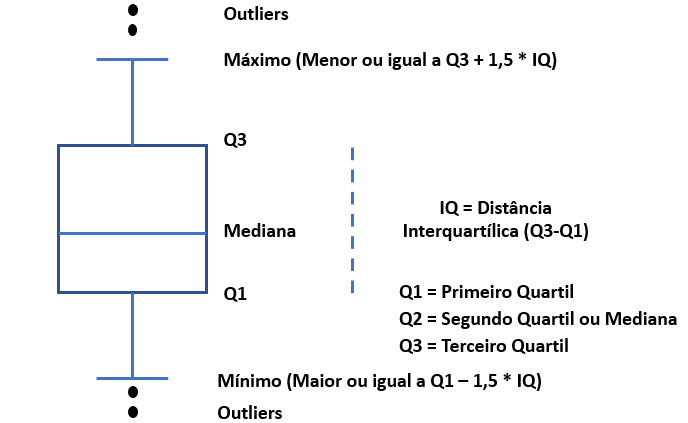
\includegraphics{./data/boxplot.png}

\begin{Shaded}
\begin{Highlighting}[]
\FunctionTok{boxplot}\NormalTok{(altura)}
\end{Highlighting}
\end{Shaded}

\includegraphics{Modulo_1_Introducao_Linguagem_R_files/figure-latex/unnamed-chunk-44-1.pdf}

\hypertarget{histograma}{%
\subsubsection{Histograma}\label{histograma}}

Utilziamos histogramas para visualizar a distribuição de uma variável
contínua. Em R o pacote ``base'' nos fornece a função \texttt{hist(\ )}.

\textbf{Exercício Prático}

\begin{itemize}
\tightlist
\item
  Mostrar o histograma para os dados da variável DAP disponível no vetor
  \texttt{dap}
\end{itemize}

\begin{Shaded}
\begin{Highlighting}[]
\FunctionTok{hist}\NormalTok{(dap)}
\end{Highlighting}
\end{Shaded}

\includegraphics{Modulo_1_Introducao_Linguagem_R_files/figure-latex/unnamed-chunk-45-1.pdf}

\hypertarget{gruxe1fico-dispersuxe3o}{%
\subsubsection{Gráfico Dispersão}\label{gruxe1fico-dispersuxe3o}}

O gráfico de dispersão é utilizado para visualizar a relação entre duas
variáveis contínuas. Para gerar um gráfico de dispersão em R devemos
utilizar a função \texttt{plot} do pacote ``base''.

\textbf{Exercício Prático}

Visualizar a relação entre a varíavel altura e diâmetro.

\begin{Shaded}
\begin{Highlighting}[]
\FunctionTok{plot}\NormalTok{(altura, dap)}
\end{Highlighting}
\end{Shaded}

\begin{center}\includegraphics{Modulo_1_Introducao_Linguagem_R_files/figure-latex/unnamed-chunk-46-1} \end{center}

\hypertarget{modificar-a-aparuxeancia-dos-gruxe1ficos}{%
\subsection{Modificar a Aparência dos
Gráficos}\label{modificar-a-aparuxeancia-dos-gruxe1ficos}}

A configuração dos parâmetros de estilo, tamanho e agrupamento dos
gráficos pode ser obtida digitando o comando ? par. Para este curso
introdutório utilizaremos apenas o básico da configuração da aparecência
de gráficos no pacote ``base'' do R.

\hypertarget{personalizando-histogramas}{%
\subsubsection{Personalizando
Histogramas}\label{personalizando-histogramas}}

\begin{itemize}
\tightlist
\item
  \texttt{main} Utilizado para atribuir ou modificar um título do
  gráfico
\end{itemize}

\begin{Shaded}
\begin{Highlighting}[]
\CommentTok{\# Modificar o título do gráfico}
\FunctionTok{hist}\NormalTok{(dap, }\AttributeTok{main =} \StringTok{\textquotesingle{}Distribuição da variável DAP (cm)\textquotesingle{}}\NormalTok{)}
\end{Highlighting}
\end{Shaded}

\begin{center}\includegraphics{Modulo_1_Introducao_Linguagem_R_files/figure-latex/unnamed-chunk-47-1} \end{center}

\begin{itemize}
\tightlist
\item
  \texttt{xlab} e \texttt{ylab} - Modificar os nomes dos eixos x e y.
\end{itemize}

\begin{Shaded}
\begin{Highlighting}[]
\CommentTok{\# Modificar os rótulos dos eixos x e y}
\FunctionTok{hist}\NormalTok{(dap, }
     \AttributeTok{main =} \StringTok{\textquotesingle{}Distribuição da variável DAP\textquotesingle{}}\NormalTok{, }\CommentTok{\# título do gráfico}
    \AttributeTok{xlab =} \StringTok{\textquotesingle{}DAP (cm)\textquotesingle{}}\NormalTok{,   }\CommentTok{\# Rótulo do eixo x}
    \AttributeTok{ylab =} \StringTok{\textquotesingle{}Frequência\textquotesingle{}}\NormalTok{) }\CommentTok{\# Rótulo do eixo y}
\end{Highlighting}
\end{Shaded}

\begin{center}\includegraphics{Modulo_1_Introducao_Linguagem_R_files/figure-latex/unnamed-chunk-48-1} \end{center}

\begin{itemize}
\tightlist
\item
  \texttt{labels} - Mostra os valores de cada barra do histograma.
\end{itemize}

\begin{Shaded}
\begin{Highlighting}[]
\FunctionTok{hist}\NormalTok{(dap, }
     \AttributeTok{main =} \StringTok{\textquotesingle{}Distribuição da variável DAP\textquotesingle{}}\NormalTok{,}
    \AttributeTok{xlab =} \StringTok{\textquotesingle{}DAP (cm)\textquotesingle{}}\NormalTok{,}
    \AttributeTok{ylab =} \StringTok{\textquotesingle{}Frequência\textquotesingle{}}\NormalTok{,}
    \AttributeTok{labels =} \ConstantTok{TRUE}\NormalTok{)}
\end{Highlighting}
\end{Shaded}

\begin{center}\includegraphics{Modulo_1_Introducao_Linguagem_R_files/figure-latex/unnamed-chunk-49-1} \end{center}

\begin{itemize}
\tightlist
\item
  \texttt{col} - Muda a cor das barras do histograma.
\end{itemize}

\begin{Shaded}
\begin{Highlighting}[]
\FunctionTok{hist}\NormalTok{(dap, }
     \AttributeTok{main =} \StringTok{\textquotesingle{}Distribuição da variável DAP\textquotesingle{}}\NormalTok{,}
    \AttributeTok{xlab =} \StringTok{\textquotesingle{}DAP (cm)\textquotesingle{}}\NormalTok{,}
    \AttributeTok{ylab =} \StringTok{\textquotesingle{}Frequência\textquotesingle{}}\NormalTok{,}
    \AttributeTok{labels =} \ConstantTok{TRUE}\NormalTok{,}
    \AttributeTok{col =} \StringTok{\textquotesingle{}darkgreen\textquotesingle{}}\NormalTok{)}
\end{Highlighting}
\end{Shaded}

\begin{center}\includegraphics{Modulo_1_Introducao_Linguagem_R_files/figure-latex/unnamed-chunk-50-1} \end{center}

\begin{itemize}
\tightlist
\item
  \texttt{density} e \texttt{angle} - Mostram as barras do histograma
  hachuradas
\end{itemize}

\begin{Shaded}
\begin{Highlighting}[]
\FunctionTok{hist}\NormalTok{(dap, }
     \AttributeTok{main =} \StringTok{\textquotesingle{}Distribuição da variável DAP\textquotesingle{}}\NormalTok{,}
    \AttributeTok{xlab =} \StringTok{\textquotesingle{}DAP (cm)\textquotesingle{}}\NormalTok{,}
    \AttributeTok{ylab =} \StringTok{\textquotesingle{}Frequência\textquotesingle{}}\NormalTok{,}
    \AttributeTok{labels =} \ConstantTok{TRUE}\NormalTok{,}
    \AttributeTok{col =} \StringTok{\textquotesingle{}steelblue\textquotesingle{}}\NormalTok{,}
    \AttributeTok{density =} \DecValTok{15}\NormalTok{,}
    \AttributeTok{angle =} \DecValTok{60}\NormalTok{)}
\end{Highlighting}
\end{Shaded}

\begin{center}\includegraphics{Modulo_1_Introducao_Linguagem_R_files/figure-latex/unnamed-chunk-51-1} \end{center}

\begin{itemize}
\tightlist
\item
  \texttt{Abline(\ )} - Função para adicionar uma linha reta ao
  histograma. Para adicionar uma linha vertical deve-se utilizar o
  argumento \texttt{v} e para linha horizontal \texttt{h}. O tipo de
  linha é modificado através do argumento \texttt{lty} (\emph{line
  type}) e a espessura da linha através do argumento \texttt{lwd}
  (\emph{line width}).
\end{itemize}

O exemplo a seguir mostra como adicionar uma linha ao histograma para
representar a média dos diâmetros.

\begin{Shaded}
\begin{Highlighting}[]
\FunctionTok{hist}\NormalTok{(dap, }
     \AttributeTok{main =} \StringTok{\textquotesingle{}Distribuição da variável DAP\textquotesingle{}}\NormalTok{,}
    \AttributeTok{xlab =} \StringTok{\textquotesingle{}DAP (cm)\textquotesingle{}}\NormalTok{,}
    \AttributeTok{ylab =} \StringTok{\textquotesingle{}Frequência\textquotesingle{}}\NormalTok{,}
    \AttributeTok{labels =} \ConstantTok{TRUE}\NormalTok{,}
    \AttributeTok{col =} \StringTok{\textquotesingle{}steelblue\textquotesingle{}}\NormalTok{,}
    \AttributeTok{density =} \DecValTok{15}\NormalTok{,}
    \AttributeTok{angle =} \DecValTok{60}\NormalTok{)}

\FunctionTok{abline}\NormalTok{(}\AttributeTok{v =} \FunctionTok{mean}\NormalTok{(dap),}
       \AttributeTok{col =} \StringTok{\textquotesingle{}red\textquotesingle{}}\NormalTok{, }
       \AttributeTok{lty =} \DecValTok{2}\NormalTok{, }
       \AttributeTok{lwd =} \DecValTok{2}\NormalTok{)}
\end{Highlighting}
\end{Shaded}

\begin{center}\includegraphics{Modulo_1_Introducao_Linguagem_R_files/figure-latex/unnamed-chunk-52-1} \end{center}

\hypertarget{personalizando-gruxe1ficos-de-dispersuxe3o}{%
\subsubsection{Personalizando Gráficos de
Dispersão}\label{personalizando-gruxe1ficos-de-dispersuxe3o}}

\begin{itemize}
\tightlist
\item
  \texttt{pch} - Altera o tipo de caractere dos pontos
\end{itemize}

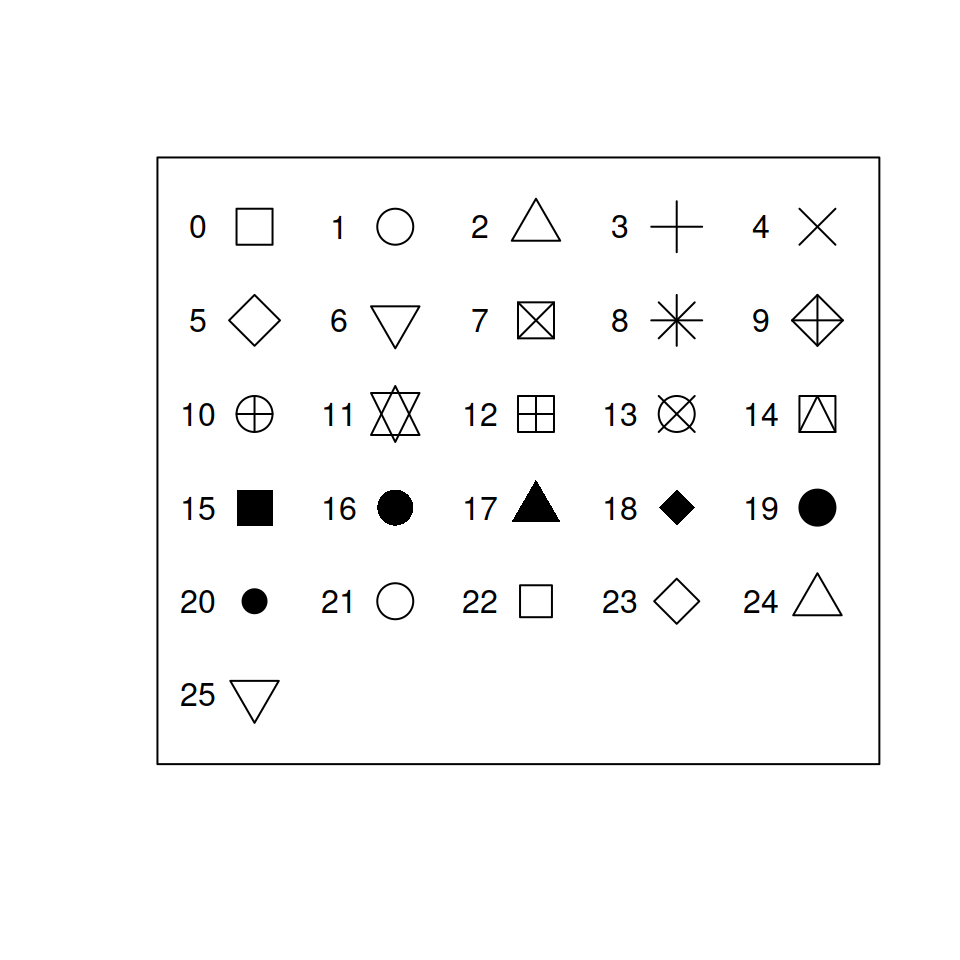
\includegraphics{./data/pch-symbols.png}

\begin{itemize}
\tightlist
\item
  Forma, Tamanho e Cor dos Pontos
\end{itemize}

\begin{longtable}[]{@{}cc@{}}
\toprule()
Argumento & Saída \\
\midrule()
\endhead
\texttt{col} & Cor da borda do ponto. \\
\texttt{bg} & Cor do Fundo do ponto. \\
\texttt{cex} & Tamanho do ponto. \\
\texttt{lwd} & Espessura da Borda do Ponto. \\
\bottomrule()
\end{longtable}

\begin{Shaded}
\begin{Highlighting}[]
\CommentTok{\# Alterar o tipo de caractere dos pontos}
\FunctionTok{plot}\NormalTok{(altura, dap, }\AttributeTok{pch =} \DecValTok{25}\NormalTok{)}
\end{Highlighting}
\end{Shaded}

\begin{center}\includegraphics{Modulo_1_Introducao_Linguagem_R_files/figure-latex/unnamed-chunk-53-1} \end{center}

\begin{itemize}
\tightlist
\item
  \texttt{las} (\emph{label style}) - Rotação dos rótulos dos eixos x e
  y.
\end{itemize}

\begin{longtable}[]{@{}cc@{}}
\toprule()
\texttt{las} & Rótulo \\
\midrule()
\endhead
0 & Paralelo aos eixos \\
1 & Sempre na Horizontal \\
2 & Sempre na Perpendicular \\
3 & Sempre na Vertical \\
\bottomrule()
\end{longtable}

\begin{Shaded}
\begin{Highlighting}[]
\FunctionTok{plot}\NormalTok{(altura, dap, }\AttributeTok{pch =} \DecValTok{21}\NormalTok{, }\AttributeTok{las =} \DecValTok{0}\NormalTok{)}
\end{Highlighting}
\end{Shaded}

\begin{center}\includegraphics{Modulo_1_Introducao_Linguagem_R_files/figure-latex/unnamed-chunk-54-1} \end{center}

\begin{Shaded}
\begin{Highlighting}[]
\FunctionTok{plot}\NormalTok{(altura, dap, }\AttributeTok{pch =} \DecValTok{21}\NormalTok{, }\AttributeTok{las =} \DecValTok{2}\NormalTok{)}
\end{Highlighting}
\end{Shaded}

\begin{center}\includegraphics{Modulo_1_Introducao_Linguagem_R_files/figure-latex/unnamed-chunk-55-1} \end{center}

\hypertarget{agrupar-gruxe1ficos-em-uma-uxfanica-figura}{%
\subsubsection{Agrupar Gráficos em uma Única
Figura}\label{agrupar-gruxe1ficos-em-uma-uxfanica-figura}}

\begin{Shaded}
\begin{Highlighting}[]
\CommentTok{\# Parâmetros gráficos}
\FunctionTok{par}\NormalTok{(}\AttributeTok{mfcol =} \FunctionTok{c}\NormalTok{(}\DecValTok{2}\NormalTok{, }\DecValTok{2}\NormalTok{))}

\FunctionTok{hist}\NormalTok{(dap, }\AttributeTok{pin =} \FunctionTok{c}\NormalTok{(}\DecValTok{12}\NormalTok{, }\DecValTok{8}\NormalTok{))}
\FunctionTok{hist}\NormalTok{(altura)}
\FunctionTok{plot}\NormalTok{(altura, dap, }\AttributeTok{pch =} \DecValTok{20}\NormalTok{)}
\FunctionTok{boxplot}\NormalTok{(dap)}
\end{Highlighting}
\end{Shaded}

\begin{center}\includegraphics{Modulo_1_Introducao_Linguagem_R_files/figure-latex/unnamed-chunk-56-1} \end{center}

\hypertarget{matriz}{%
\section{Matriz}\label{matriz}}

Matriz é uma estrutura de dados semelhante a vetor, exceto que na matriz
temos 2 dimensões, uma para as linhas e outra para as colunas. O código
a seguir mostra a criação de uma matriz 3x3.

\begin{Shaded}
\begin{Highlighting}[]
\NormalTok{matriz }\OtherTok{\textless{}{-}} \FunctionTok{matrix}\NormalTok{(}\DecValTok{1}\SpecialCharTok{:}\DecValTok{9}\NormalTok{, }\AttributeTok{nrow =} \DecValTok{3}\NormalTok{, }\AttributeTok{ncol =} \DecValTok{3}\NormalTok{)}
\NormalTok{matriz}
\end{Highlighting}
\end{Shaded}

\begin{verbatim}
##      [,1] [,2] [,3]
## [1,]    1    4    7
## [2,]    2    5    8
## [3,]    3    6    9
\end{verbatim}

\hypertarget{somar-linhas-e-colunas-de-uma-matriz}{%
\subsection{Somar linhas e Colunas de uma
Matriz}\label{somar-linhas-e-colunas-de-uma-matriz}}

A função \texttt{apply}, parte do pacote \texttt{base} do R, pode ser
usada para aplicar uma determinada função a uma matriz, e recebe 3
argumentos como parâmetro: a matriz contendo os dados, a indicação do
sentido de aplicação da função, representado pelos números 1 (linha) ou
2 (coluna) e a função a ser aplicada.

Somar as linhas de uma matriz:

\begin{Shaded}
\begin{Highlighting}[]
\FunctionTok{print}\NormalTok{(}\FunctionTok{apply}\NormalTok{(matriz, }\DecValTok{1}\NormalTok{, sum))}
\end{Highlighting}
\end{Shaded}

\begin{verbatim}
## [1] 12 15 18
\end{verbatim}

Somar os valores das colunas de uma matriz:

\begin{Shaded}
\begin{Highlighting}[]
\FunctionTok{print}\NormalTok{(}\FunctionTok{apply}\NormalTok{(matriz, }\DecValTok{2}\NormalTok{, sum))}
\end{Highlighting}
\end{Shaded}

\begin{verbatim}
## [1]  6 15 24
\end{verbatim}

\hypertarget{somar-os-elementos-da-diagonal-de-uma-matriz}{%
\subsection{Somar os Elementos da Diagonal de uma
Matriz}\label{somar-os-elementos-da-diagonal-de-uma-matriz}}

\begin{Shaded}
\begin{Highlighting}[]
\NormalTok{m }\OtherTok{\textless{}{-}} \FunctionTok{matrix}\NormalTok{(}\DecValTok{1}\SpecialCharTok{:}\DecValTok{9}\NormalTok{, }\AttributeTok{nrow =} \DecValTok{3}\NormalTok{, }\AttributeTok{ncol =} \DecValTok{3}\NormalTok{)}
\FunctionTok{print}\NormalTok{(m)}
\end{Highlighting}
\end{Shaded}

\begin{verbatim}
##      [,1] [,2] [,3]
## [1,]    1    4    7
## [2,]    2    5    8
## [3,]    3    6    9
\end{verbatim}

\begin{Shaded}
\begin{Highlighting}[]
\FunctionTok{sum}\NormalTok{(}\FunctionTok{diag}\NormalTok{(m))}
\end{Highlighting}
\end{Shaded}

\begin{verbatim}
## [1] 15
\end{verbatim}

\hypertarget{sentido-de-preenchimento-dos-dados-em-uma-matriz}{%
\subsection{Sentido de Preenchimento dos Dados em uma
Matriz}\label{sentido-de-preenchimento-dos-dados-em-uma-matriz}}

A função \texttt{matrix()} tem por padrão o preenchimento no sentido das
colunas, porém, em alguns casos podemos necessitar preencher uma matriz
no sentido das linhas, para isso devemos definir o valor do argumento
\texttt{byrow\ =\ TRUE}

\begin{Shaded}
\begin{Highlighting}[]
\NormalTok{matriz }\OtherTok{\textless{}{-}} \FunctionTok{matrix}\NormalTok{(}\DecValTok{1}\SpecialCharTok{:}\DecValTok{9}\NormalTok{, }\AttributeTok{nrow =} \DecValTok{3}\NormalTok{, }\AttributeTok{ncol =} \DecValTok{3}\NormalTok{, }\AttributeTok{byrow =} \ConstantTok{TRUE}\NormalTok{)}
\FunctionTok{print}\NormalTok{(matriz)}
\end{Highlighting}
\end{Shaded}

\begin{verbatim}
##      [,1] [,2] [,3]
## [1,]    1    2    3
## [2,]    4    5    6
## [3,]    7    8    9
\end{verbatim}

\hypertarget{atribuir-nomes-as-linhas-e-colunas-de-uma-matriz}{%
\subsection{Atribuir Nomes as Linhas e Colunas de uma
Matriz}\label{atribuir-nomes-as-linhas-e-colunas-de-uma-matriz}}

\begin{Shaded}
\begin{Highlighting}[]
\NormalTok{matriz }\OtherTok{\textless{}{-}} \FunctionTok{matrix}\NormalTok{(}\DecValTok{1}\SpecialCharTok{:}\DecValTok{9}\NormalTok{, }\AttributeTok{nrow =} \DecValTok{3}\NormalTok{, }\AttributeTok{ncol =} \DecValTok{3}\NormalTok{, }\AttributeTok{byrow =} \ConstantTok{TRUE}\NormalTok{)}
\FunctionTok{print}\NormalTok{(matriz)}
\end{Highlighting}
\end{Shaded}

\begin{verbatim}
##      [,1] [,2] [,3]
## [1,]    1    2    3
## [2,]    4    5    6
## [3,]    7    8    9
\end{verbatim}

\begin{Shaded}
\begin{Highlighting}[]
\CommentTok{\# Atribuir Nomes as Linhas da matriz}
\FunctionTok{rownames}\NormalTok{(matriz) }\OtherTok{\textless{}{-}} \FunctionTok{c}\NormalTok{(}\StringTok{\textquotesingle{}Linha 1\textquotesingle{}}\NormalTok{, }\StringTok{\textquotesingle{}Linha 2\textquotesingle{}}\NormalTok{, }\StringTok{\textquotesingle{}Linha 3\textquotesingle{}}\NormalTok{)}
\end{Highlighting}
\end{Shaded}

\begin{Shaded}
\begin{Highlighting}[]
\FunctionTok{print}\NormalTok{(matriz)}
\end{Highlighting}
\end{Shaded}

\begin{verbatim}
##         [,1] [,2] [,3]
## Linha 1    1    2    3
## Linha 2    4    5    6
## Linha 3    7    8    9
\end{verbatim}

\begin{Shaded}
\begin{Highlighting}[]
\CommentTok{\# Atribuir Nomes as colunas da matriz}
\FunctionTok{colnames}\NormalTok{(matriz) }\OtherTok{\textless{}{-}} \FunctionTok{c}\NormalTok{(}\StringTok{\textquotesingle{}Coluna 1\textquotesingle{}}\NormalTok{, }\StringTok{\textquotesingle{}Coluna 2\textquotesingle{}}\NormalTok{, }\StringTok{\textquotesingle{}Coluna 3\textquotesingle{}}\NormalTok{)}
\end{Highlighting}
\end{Shaded}

\begin{Shaded}
\begin{Highlighting}[]
\NormalTok{matriz}
\end{Highlighting}
\end{Shaded}

\begin{verbatim}
##         Coluna 1 Coluna 2 Coluna 3
## Linha 1        1        2        3
## Linha 2        4        5        6
## Linha 3        7        8        9
\end{verbatim}

\hypertarget{obter-os-nomes-das-linhas-e-colunas-de-uma-matriz}{%
\subsection{Obter os nomes das Linhas e Colunas de uma
Matriz}\label{obter-os-nomes-das-linhas-e-colunas-de-uma-matriz}}

\textbf{Somente os Nomes das Linhas}

\begin{Shaded}
\begin{Highlighting}[]
\FunctionTok{rownames}\NormalTok{(matriz)}
\end{Highlighting}
\end{Shaded}

\begin{verbatim}
## [1] "Linha 1" "Linha 2" "Linha 3"
\end{verbatim}

\textbf{Somente os Nomes das Colunas}

\begin{Shaded}
\begin{Highlighting}[]
\FunctionTok{colnames}\NormalTok{(matriz)}
\end{Highlighting}
\end{Shaded}

\begin{verbatim}
## [1] "Coluna 1" "Coluna 2" "Coluna 3"
\end{verbatim}

\textbf{Nomes das Linhas e Colunas}

\begin{Shaded}
\begin{Highlighting}[]
\FunctionTok{dimnames}\NormalTok{(matriz)}
\end{Highlighting}
\end{Shaded}

\begin{verbatim}
## [[1]]
## [1] "Linha 1" "Linha 2" "Linha 3"
## 
## [[2]]
## [1] "Coluna 1" "Coluna 2" "Coluna 3"
\end{verbatim}

\hypertarget{acessar-linhas-e-colunas-da-matriz}{%
\subsection{Acessar Linhas e Colunas da
Matriz}\label{acessar-linhas-e-colunas-da-matriz}}

\begin{Shaded}
\begin{Highlighting}[]
\CommentTok{\# mostrar a primeira linha da matriz}
\FunctionTok{print}\NormalTok{(matriz[}\DecValTok{1}\NormalTok{, ])}
\end{Highlighting}
\end{Shaded}

\begin{verbatim}
## Coluna 1 Coluna 2 Coluna 3 
##        1        2        3
\end{verbatim}

\begin{Shaded}
\begin{Highlighting}[]
\CommentTok{\# mostrar a segunda Coluna da matriz}
\FunctionTok{print}\NormalTok{(matriz[, }\DecValTok{2}\NormalTok{])}
\end{Highlighting}
\end{Shaded}

\begin{verbatim}
## Linha 1 Linha 2 Linha 3 
##       2       5       8
\end{verbatim}

\hypertarget{acessar-elementos-da-matriz}{%
\subsection{Acessar Elementos da
Matriz}\label{acessar-elementos-da-matriz}}

\begin{Shaded}
\begin{Highlighting}[]
\CommentTok{\# Mostrar o elemento pertencente a segunda linha e segunda coluna}
\FunctionTok{print}\NormalTok{(matriz[}\DecValTok{2}\NormalTok{, }\DecValTok{2}\NormalTok{])}
\end{Highlighting}
\end{Shaded}

\begin{verbatim}
## [1] 5
\end{verbatim}

\hypertarget{alterar-os-elementos-de-uma-matriz}{%
\subsection{Alterar os Elementos de uma
Matriz}\label{alterar-os-elementos-de-uma-matriz}}

\begin{Shaded}
\begin{Highlighting}[]
\CommentTok{\# alterar o elemento da linha 2 coluna 2, número 5, para 0}
\NormalTok{matriz[}\DecValTok{2}\NormalTok{, }\DecValTok{2}\NormalTok{] }\OtherTok{\textless{}{-}} \DecValTok{0}
\FunctionTok{print}\NormalTok{(matriz)}
\end{Highlighting}
\end{Shaded}

\begin{verbatim}
##         Coluna 1 Coluna 2 Coluna 3
## Linha 1        1        2        3
## Linha 2        4        0        6
## Linha 3        7        8        9
\end{verbatim}

\hypertarget{operauxe7uxf5es-com-matrizes}{%
\subsection{Operações com Matrizes}\label{operauxe7uxf5es-com-matrizes}}

\hypertarget{maior-e-menor-valor-entre-os-elementos-da-matriz}{%
\subsubsection{\texorpdfstring{\textbf{Maior e menor valor entre os
elementos da
matriz}}{Maior e menor valor entre os elementos da matriz}}\label{maior-e-menor-valor-entre-os-elementos-da-matriz}}

\begin{Shaded}
\begin{Highlighting}[]
\CommentTok{\# maior valor entre os elementos da matriz}
\FunctionTok{max}\NormalTok{(matriz)}
\end{Highlighting}
\end{Shaded}

\begin{verbatim}
## [1] 9
\end{verbatim}

\begin{Shaded}
\begin{Highlighting}[]
\CommentTok{\# menor valor entre os elementos da matriz}
\FunctionTok{min}\NormalTok{(matriz)}
\end{Highlighting}
\end{Shaded}

\begin{verbatim}
## [1] 0
\end{verbatim}

\hypertarget{maior-e-menor-valor-de-uma-linha-ou-coluna-da-matriz}{%
\subsubsection{\texorpdfstring{\textbf{Maior e menor valor de uma linha
ou coluna da
matriz}}{Maior e menor valor de uma linha ou coluna da matriz}}\label{maior-e-menor-valor-de-uma-linha-ou-coluna-da-matriz}}

\begin{Shaded}
\begin{Highlighting}[]
\CommentTok{\# maior valor entre os elementos da primeira linha}
\FunctionTok{max}\NormalTok{(matriz[}\DecValTok{1}\NormalTok{,])}
\end{Highlighting}
\end{Shaded}

\begin{verbatim}
## [1] 3
\end{verbatim}

\begin{Shaded}
\begin{Highlighting}[]
\CommentTok{\# menor valor entre os elementos da terceira coluna}
\FunctionTok{min}\NormalTok{(matriz[,}\DecValTok{3}\NormalTok{])}
\end{Highlighting}
\end{Shaded}

\begin{verbatim}
## [1] 3
\end{verbatim}

\hypertarget{muxe9dia-dos-elementos-da-matriz}{%
\subsubsection{\texorpdfstring{\textbf{Média dos elementos da
matriz}}{Média dos elementos da matriz}}\label{muxe9dia-dos-elementos-da-matriz}}

\begin{Shaded}
\begin{Highlighting}[]
\FunctionTok{mean}\NormalTok{(matriz)}
\end{Highlighting}
\end{Shaded}

\begin{verbatim}
## [1] 4.444444
\end{verbatim}

\hypertarget{somar-os-valores-das-linhas-e-colunas}{%
\subsubsection{\texorpdfstring{\textbf{Somar os valores das linhas e
colunas}}{Somar os valores das linhas e colunas}}\label{somar-os-valores-das-linhas-e-colunas}}

\hypertarget{soma-de-elementos-da-matriz}{%
\subsubsection{\texorpdfstring{\textbf{Soma de elementos da
matriz}}{Soma de elementos da matriz}}\label{soma-de-elementos-da-matriz}}

\begin{Shaded}
\begin{Highlighting}[]
\CommentTok{\# somar os valores da primeira linha}
\FunctionTok{sum}\NormalTok{(matriz[}\DecValTok{1}\NormalTok{, ])}
\end{Highlighting}
\end{Shaded}

\begin{verbatim}
## [1] 6
\end{verbatim}

\begin{Shaded}
\begin{Highlighting}[]
\CommentTok{\# somar os valores da terceira coluna}
\FunctionTok{sum}\NormalTok{(matriz[, }\DecValTok{3}\NormalTok{])}
\end{Highlighting}
\end{Shaded}

\begin{verbatim}
## [1] 18
\end{verbatim}

\begin{Shaded}
\begin{Highlighting}[]
\CommentTok{\# somar os elementos da segunda linha da matriz}
\FunctionTok{sum}\NormalTok{(matriz[}\DecValTok{2}\NormalTok{, ])}
\end{Highlighting}
\end{Shaded}

\begin{verbatim}
## [1] 10
\end{verbatim}

\hypertarget{diagonal-da-matriz}{%
\subsubsection{\texorpdfstring{\textbf{Diagonal da
matriz}}{Diagonal da matriz}}\label{diagonal-da-matriz}}

\begin{Shaded}
\begin{Highlighting}[]
\CommentTok{\# Obter a diagonal da matriz}
\FunctionTok{print}\NormalTok{(}\FunctionTok{diag}\NormalTok{(matriz))}
\end{Highlighting}
\end{Shaded}

\begin{verbatim}
## [1] 1 0 9
\end{verbatim}

\begin{Shaded}
\begin{Highlighting}[]
\CommentTok{\# Obter a soma entre os elementos da diagonal da matriz}
\FunctionTok{sum}\NormalTok{(}\FunctionTok{diag}\NormalTok{(matriz))}
\end{Highlighting}
\end{Shaded}

\begin{verbatim}
## [1] 10
\end{verbatim}

\hypertarget{transposiuxe7uxe3o-de-matriz}{%
\subsubsection{\texorpdfstring{\textbf{Transposição de
Matriz}}{Transposição de Matriz}}\label{transposiuxe7uxe3o-de-matriz}}

\begin{Shaded}
\begin{Highlighting}[]
\CommentTok{\# Transpor a matriz}
\FunctionTok{t}\NormalTok{(matriz)}
\end{Highlighting}
\end{Shaded}

\begin{verbatim}
##          Linha 1 Linha 2 Linha 3
## Coluna 1       1       4       7
## Coluna 2       2       0       8
## Coluna 3       3       6       9
\end{verbatim}

\hypertarget{soma-entre-matrizes}{%
\subsubsection{\texorpdfstring{\textbf{Soma entre
matrizes}}{Soma entre matrizes}}\label{soma-entre-matrizes}}

\begin{Shaded}
\begin{Highlighting}[]
\CommentTok{\# Definição das matrizes "a" e "b"}
\NormalTok{a }\OtherTok{\textless{}{-}} \FunctionTok{matrix}\NormalTok{(}\DecValTok{1}\SpecialCharTok{:}\DecValTok{6}\NormalTok{, }\AttributeTok{nrow =} \DecValTok{3}\NormalTok{, }\AttributeTok{byrow =} \ConstantTok{TRUE}\NormalTok{)}
\NormalTok{b }\OtherTok{\textless{}{-}} \FunctionTok{matrix}\NormalTok{(}\DecValTok{1}\SpecialCharTok{:}\DecValTok{6}\NormalTok{, }\AttributeTok{nrow =} \DecValTok{3}\NormalTok{, }\AttributeTok{byrow =} \ConstantTok{TRUE}\NormalTok{)}

\FunctionTok{print}\NormalTok{(a)}
\end{Highlighting}
\end{Shaded}

\begin{verbatim}
##      [,1] [,2]
## [1,]    1    2
## [2,]    3    4
## [3,]    5    6
\end{verbatim}

\begin{Shaded}
\begin{Highlighting}[]
\FunctionTok{print}\NormalTok{(b)}
\end{Highlighting}
\end{Shaded}

\begin{verbatim}
##      [,1] [,2]
## [1,]    1    2
## [2,]    3    4
## [3,]    5    6
\end{verbatim}

\begin{Shaded}
\begin{Highlighting}[]
\CommentTok{\# soma das matrizes a e b}
\NormalTok{a }\SpecialCharTok{+}\NormalTok{ b}
\end{Highlighting}
\end{Shaded}

\begin{verbatim}
##      [,1] [,2]
## [1,]    2    4
## [2,]    6    8
## [3,]   10   12
\end{verbatim}

\hypertarget{combinar-vetores-em-matriz}{%
\subsection{Combinar Vetores em
Matriz}\label{combinar-vetores-em-matriz}}

Em R podemos combinar vetores para formar uma matriz em que cada vetor
fará parte de uma coluna ou linha da matriz. Para combinar vetores em
linhas matriciais usamos a função \texttt{rbind()}, e para combinar
vetores em colunas da matriz usamos a função \texttt{cbind()}. O exemplo
a seguir mostra como combinas três vetores com orientação nas linhas de
uma matriz.

\begin{Shaded}
\begin{Highlighting}[]
\CommentTok{\# Vetor referente a uma amostra de valores de ações da Apple}
\NormalTok{apple }\OtherTok{\textless{}{-}} \FunctionTok{c}\NormalTok{(}\FloatTok{109.49}\NormalTok{, }\FloatTok{109.90}\NormalTok{, }\FloatTok{109.11}\NormalTok{, }\FloatTok{109.95}\NormalTok{, }\FloatTok{111.03}\NormalTok{)}

\CommentTok{\# Vetor referente a uma amostra de valores de ações da IBM}
\NormalTok{ibm }\OtherTok{\textless{}{-}} \FunctionTok{c}\NormalTok{(}\FloatTok{159.82}\NormalTok{, }\FloatTok{160.02}\NormalTok{, }\FloatTok{159.84}\NormalTok{, }\FloatTok{160.35}\NormalTok{, }\FloatTok{164.79}\NormalTok{)}

\CommentTok{\# Vetor referente a uma amostra de valores de ações da Microsoft}
\NormalTok{microsoft }\OtherTok{\textless{}{-}} \FunctionTok{c}\NormalTok{(}\FloatTok{59.20}\NormalTok{, }\FloatTok{59.25}\NormalTok{, }\FloatTok{60.22}\NormalTok{, }\FloatTok{59.95}\NormalTok{, }\FloatTok{61.37}\NormalTok{)}

\CommentTok{\# combinar os vetores em uma matriz onde cada linha receberá os valores dos vetores}
\FunctionTok{print}\NormalTok{(}\FunctionTok{rbind}\NormalTok{(apple, ibm, microsoft))}
\end{Highlighting}
\end{Shaded}

\begin{verbatim}
##             [,1]   [,2]   [,3]   [,4]   [,5]
## apple     109.49 109.90 109.11 109.95 111.03
## ibm       159.82 160.02 159.84 160.35 164.79
## microsoft  59.20  59.25  60.22  59.95  61.37
\end{verbatim}

A seguir é demonstrado como combinar os elementos de vetores em colunas
de uma matriz.

\begin{Shaded}
\begin{Highlighting}[]
\CommentTok{\# combinar os vetores em uma matriz onde cada coluna receberá os valores dos vetores}
\FunctionTok{cbind}\NormalTok{(apple, ibm, microsoft)}
\end{Highlighting}
\end{Shaded}

\begin{verbatim}
##       apple    ibm microsoft
## [1,] 109.49 159.82     59.20
## [2,] 109.90 160.02     59.25
## [3,] 109.11 159.84     60.22
## [4,] 109.95 160.35     59.95
## [5,] 111.03 164.79     61.37
\end{verbatim}

\hypertarget{matriz-de-correlauxe7uxe3o}{%
\subsection{Matriz de Correlação}\label{matriz-de-correlauxe7uxe3o}}

Como exemplo prático para demonstrar o uso de matriz para cálcular a
correlação entre variáveis, usaremos os dados referente a publicação:

Ramsey, F.L. and Schafer, D.W. (2013). \emph{The Statistical Sleuth}: A
Course in Methods of Data Analysis (3rd ed), Cengage Learning.

Os dados são os valores médios de peso cerebral (g), peso corporal (g),
duração da gestação (dias) e tamanho da prole de 96 espécies de
mamíferos.

\begin{Shaded}
\begin{Highlighting}[]
\CommentTok{\# Carregar os dados vetoriais}
\FunctionTok{load}\NormalTok{(}\StringTok{\textquotesingle{}./data/dados\_modulo\_1\_aula\_3.rda\textquotesingle{}}\NormalTok{)}

\CommentTok{\# listar os objetos no ambiente R}
\FunctionTok{ls}\NormalTok{()}
\end{Highlighting}
\end{Shaded}

\begin{verbatim}
##  [1] "a"                 "altura"            "apple"            
##  [4] "b"                 "categoria"         "cerebro"          
##  [7] "corpo"             "dap"               "dias_semana"      
## [10] "especies"          "gestacao"          "ibm"              
## [13] "int"               "inteiros"          "letra"            
## [16] "m"                 "matriz"            "microsoft"        
## [19] "nomes"             "nomes_cientificos" "num"              
## [22] "prole"             "sequencia"         "string"           
## [25] "temperatura"       "vetor"
\end{verbatim}

\begin{Shaded}
\begin{Highlighting}[]
\CommentTok{\# Combinar os vetores em uma matriz}
\NormalTok{m }\OtherTok{\textless{}{-}} \FunctionTok{cbind}\NormalTok{(cerebro, corpo, gestacao, prole)}

\CommentTok{\# Mostrar as primeiras 6 linhas da matriz}
\FunctionTok{head}\NormalTok{(m)}
\end{Highlighting}
\end{Shaded}

\begin{verbatim}
##      cerebro   corpo gestacao prole
## [1,]     9.6    2.20       31   5.0
## [2,]     9.9    0.78       98   1.2
## [3,]  4480.0 2800.00      655   1.0
## [4,]    20.3    2.80      104   1.3
## [5,]   219.0   89.00      218   1.0
## [6,]    53.0    6.00       60   2.2
\end{verbatim}

\begin{Shaded}
\begin{Highlighting}[]
\CommentTok{\# Mostrar as últimas 6 linhas da matriz}
\FunctionTok{tail}\NormalTok{(m)}
\end{Highlighting}
\end{Shaded}

\begin{verbatim}
##       cerebro corpo gestacao prole
## [91,]     198  45.0      300   1.1
## [92,]     550 400.0      310   1.0
## [93,]     179  32.0      180   1.0
## [94,]     102   5.5      210   1.0
## [95,]     185 150.0      120   4.0
## [96,]     334 250.0      255   1.0
\end{verbatim}

\hypertarget{atribuir-um-atributo-a-uma-matriz}{%
\subsection{Atribuir um Atributo a uma
Matriz}\label{atribuir-um-atributo-a-uma-matriz}}

Para inserir um atributo a matriz utilizamos a função \texttt{attr()},
passando como argumentos a matriz e um rótulo para nomear o atributo.
Como demonstração iremos inserir um atributo a nossa matriz definida
anteriormente, este atributo será a referência bibliográfica dos dados.

\begin{Shaded}
\begin{Highlighting}[]
\CommentTok{\# Obter os atributos da matriz}
\FunctionTok{attributes}\NormalTok{(m)}
\end{Highlighting}
\end{Shaded}

\begin{verbatim}
## $dim
## [1] 96  4
## 
## $dimnames
## $dimnames[[1]]
## NULL
## 
## $dimnames[[2]]
## [1] "cerebro"  "corpo"    "gestacao" "prole"
\end{verbatim}

\begin{Shaded}
\begin{Highlighting}[]
\CommentTok{\# Inserir o atributo}
\FunctionTok{attr}\NormalTok{(m, }\StringTok{\textquotesingle{}Fonte\textquotesingle{}}\NormalTok{) }\OtherTok{\textless{}{-}} \StringTok{\textquotesingle{}Ramsey, F.L. and Schafer, D.W. (2013). The Statistical Sleuth: A Course in Methods of Data Analysis (3rd ed), Cengage Learning.\textquotesingle{}}
\end{Highlighting}
\end{Shaded}

\begin{Shaded}
\begin{Highlighting}[]
\CommentTok{\# conferir os atributos da matriz}
\FunctionTok{attributes}\NormalTok{(m)}
\end{Highlighting}
\end{Shaded}

\begin{verbatim}
## $dim
## [1] 96  4
## 
## $dimnames
## $dimnames[[1]]
## NULL
## 
## $dimnames[[2]]
## [1] "cerebro"  "corpo"    "gestacao" "prole"   
## 
## 
## $Fonte
## [1] "Ramsey, F.L. and Schafer, D.W. (2013). The Statistical Sleuth: A Course in Methods of Data Analysis (3rd ed), Cengage Learning."
\end{verbatim}

\hypertarget{gerar-gruxe1ficos-a-partir-dos-dados-de-uma-matriz}{%
\subsection{Gerar Gráficos a partir dos Dados de uma
Matriz}\label{gerar-gruxe1ficos-a-partir-dos-dados-de-uma-matriz}}

\begin{Shaded}
\begin{Highlighting}[]
\CommentTok{\# gráfico da relação entre as duas primeiras colunas (cerebro e corpo)}
\FunctionTok{plot}\NormalTok{(m)}
\end{Highlighting}
\end{Shaded}

\includegraphics{Modulo_1_Introducao_Linguagem_R_files/figure-latex/unnamed-chunk-95-1.pdf}

\begin{Shaded}
\begin{Highlighting}[]
\CommentTok{\# gráfico da relação entre as duas primeiras colunas (gestacao e prole) }
\CommentTok{\# plot(m[, 3], m[, 4])}
\FunctionTok{plot}\NormalTok{(m[,}\StringTok{\textquotesingle{}gestacao\textquotesingle{}}\NormalTok{], m[,}\StringTok{\textquotesingle{}prole\textquotesingle{}}\NormalTok{])}
\end{Highlighting}
\end{Shaded}

\includegraphics{Modulo_1_Introducao_Linguagem_R_files/figure-latex/unnamed-chunk-96-1.pdf}

\hypertarget{array}{%
\section{Array}\label{array}}

Em R array é uma estrutura de dados tridimensional. Criamos um array
através da função \texttt{array(x,\ dim)}, onde o parâmetros \texttt{x}
é um vetor e \texttt{dim} são as dimensões do array.

\begin{Shaded}
\begin{Highlighting}[]
\NormalTok{a }\OtherTok{\textless{}{-}} \FunctionTok{array}\NormalTok{(}\FunctionTok{c}\NormalTok{(}\DecValTok{1}\SpecialCharTok{:}\DecValTok{24}\NormalTok{), }\AttributeTok{dim =} \FunctionTok{c}\NormalTok{(}\DecValTok{3}\NormalTok{, }\DecValTok{3}\NormalTok{, }\DecValTok{2}\NormalTok{))}
\end{Highlighting}
\end{Shaded}

\begin{Shaded}
\begin{Highlighting}[]
\FunctionTok{print}\NormalTok{(a)}
\end{Highlighting}
\end{Shaded}

\begin{verbatim}
## , , 1
## 
##      [,1] [,2] [,3]
## [1,]    1    4    7
## [2,]    2    5    8
## [3,]    3    6    9
## 
## , , 2
## 
##      [,1] [,2] [,3]
## [1,]   10   13   16
## [2,]   11   14   17
## [3,]   12   15   18
\end{verbatim}

\hypertarget{acessar-elementos-do-array}{%
\subsection{Acessar Elementos do
Array}\label{acessar-elementos-do-array}}

\begin{Shaded}
\begin{Highlighting}[]
\CommentTok{\# Acessar a primeira tabela}
\NormalTok{a[, , }\DecValTok{1}\NormalTok{]}
\end{Highlighting}
\end{Shaded}

\begin{verbatim}
##      [,1] [,2] [,3]
## [1,]    1    4    7
## [2,]    2    5    8
## [3,]    3    6    9
\end{verbatim}

\begin{Shaded}
\begin{Highlighting}[]
\CommentTok{\# Acessar a primeira linha da tabela 1}
\FunctionTok{print}\NormalTok{(a[}\DecValTok{1}\NormalTok{, , }\DecValTok{1}\NormalTok{])}
\end{Highlighting}
\end{Shaded}

\begin{verbatim}
## [1] 1 4 7
\end{verbatim}

\begin{Shaded}
\begin{Highlighting}[]
\CommentTok{\# Acessar a primeira coluna da segunda tabela}
\FunctionTok{print}\NormalTok{(a[, }\DecValTok{1}\NormalTok{, }\DecValTok{2}\NormalTok{])}
\end{Highlighting}
\end{Shaded}

\begin{verbatim}
## [1] 10 11 12
\end{verbatim}

\hypertarget{operauxe7uxf5es-com-arrays}{%
\subsection{Operações com Arrays}\label{operauxe7uxf5es-com-arrays}}

\begin{Shaded}
\begin{Highlighting}[]
\CommentTok{\# Obter o maior valor da primeira tabela}
\FunctionTok{max}\NormalTok{(a[, , }\DecValTok{1}\NormalTok{])}
\end{Highlighting}
\end{Shaded}

\begin{verbatim}
## [1] 9
\end{verbatim}

\begin{Shaded}
\begin{Highlighting}[]
\CommentTok{\# Obter a soma da primeira coluna da tabela 1}
\FunctionTok{sum}\NormalTok{(a[, }\DecValTok{1}\NormalTok{, }\DecValTok{1}\NormalTok{])}
\end{Highlighting}
\end{Shaded}

\begin{verbatim}
## [1] 6
\end{verbatim}

\begin{Shaded}
\begin{Highlighting}[]
\CommentTok{\# obter a média dos valores da segunda linha da segunda tabela}
\FunctionTok{mean}\NormalTok{(a[, }\DecValTok{2}\NormalTok{, }\DecValTok{2}\NormalTok{])}
\end{Highlighting}
\end{Shaded}

\begin{verbatim}
## [1] 14
\end{verbatim}

\begin{Shaded}
\begin{Highlighting}[]
\CommentTok{\# Obter a soma entre os valores da primeira coluna da table 1 com os da}
\CommentTok{\# primeira coluna da tabela 2}
\FunctionTok{sum}\NormalTok{(a[, }\DecValTok{1}\NormalTok{, }\DecValTok{1}\NormalTok{], a[, }\DecValTok{1}\NormalTok{, }\DecValTok{2}\NormalTok{])}
\end{Highlighting}
\end{Shaded}

\begin{verbatim}
## [1] 39
\end{verbatim}

\begin{Shaded}
\begin{Highlighting}[]
\CommentTok{\# obter a soma dos valores da diagonal da primeira tabele}
\FunctionTok{sum}\NormalTok{(}\FunctionTok{diag}\NormalTok{(a[, , }\DecValTok{1}\NormalTok{]))}
\end{Highlighting}
\end{Shaded}

\begin{verbatim}
## [1] 15
\end{verbatim}

\hypertarget{atribuir-nomes-as-dimensuxf5es-do-array}{%
\subsection{Atribuir Nomes as Dimensões do
Array}\label{atribuir-nomes-as-dimensuxf5es-do-array}}

Assim como podemos atribuir nomes aos elementos de um vetor e as duas
dimensões de uma matriz, também é possível o fazer para arrays. Para tal
utilizamos a função \texttt{dimnames()}, passando como parâmetros três
vetores com os nomes das linhas da matriz, nomes das colunas e nomes das
matrizes.

\begin{Shaded}
\begin{Highlighting}[]
\NormalTok{a }\OtherTok{\textless{}{-}} \FunctionTok{array}\NormalTok{(}\FunctionTok{c}\NormalTok{(}\DecValTok{1}\SpecialCharTok{:}\DecValTok{24}\NormalTok{),  }\CommentTok{\# Vetor}
           \AttributeTok{dim =} \FunctionTok{c}\NormalTok{(}\DecValTok{3}\NormalTok{, }\DecValTok{3}\NormalTok{, }\DecValTok{2}\NormalTok{),  }\CommentTok{\# Dimensões do array }
           \AttributeTok{dimnames =} \FunctionTok{list}\NormalTok{(}\FunctionTok{c}\NormalTok{(}\StringTok{\textquotesingle{}L1\textquotesingle{}}\NormalTok{, }\StringTok{\textquotesingle{}L2\textquotesingle{}}\NormalTok{, }\StringTok{\textquotesingle{}L3\textquotesingle{}}\NormalTok{),  }\CommentTok{\# Nome das linhas das matrizes}
                           \FunctionTok{c}\NormalTok{(}\StringTok{\textquotesingle{}C1\textquotesingle{}}\NormalTok{, }\StringTok{\textquotesingle{}C2\textquotesingle{}}\NormalTok{, }\StringTok{\textquotesingle{}C3\textquotesingle{}}\NormalTok{),  }\CommentTok{\# Nome das colunas das matrizes}
                           \FunctionTok{c}\NormalTok{(}\StringTok{\textquotesingle{}Matriz 1\textquotesingle{}}\NormalTok{, }\StringTok{\textquotesingle{}Matriz 2\textquotesingle{}}\NormalTok{)))  }\CommentTok{\# Nomes das Matrizes}

\FunctionTok{print}\NormalTok{(a)}
\end{Highlighting}
\end{Shaded}

\begin{verbatim}
## , , Matriz 1
## 
##    C1 C2 C3
## L1  1  4  7
## L2  2  5  8
## L3  3  6  9
## 
## , , Matriz 2
## 
##    C1 C2 C3
## L1 10 13 16
## L2 11 14 17
## L3 12 15 18
\end{verbatim}

\hypertarget{inserir-atributo-em-um-array}{%
\subsection{Inserir Atributo em um
Array}\label{inserir-atributo-em-um-array}}

\begin{Shaded}
\begin{Highlighting}[]
\CommentTok{\# inserir um atributo ao array "a"}
\FunctionTok{attr}\NormalTok{(a, }\StringTok{\textquotesingle{}Observação\textquotesingle{}}\NormalTok{) }\OtherTok{\textless{}{-}} \StringTok{\textquotesingle{}Meu primeiro array em R!!\textquotesingle{}}
\end{Highlighting}
\end{Shaded}

\begin{Shaded}
\begin{Highlighting}[]
\CommentTok{\# checar os atributos do array}
\FunctionTok{print}\NormalTok{(}\FunctionTok{attributes}\NormalTok{(a))}
\end{Highlighting}
\end{Shaded}

\begin{verbatim}
## $dim
## [1] 3 3 2
## 
## $dimnames
## $dimnames[[1]]
## [1] "L1" "L2" "L3"
## 
## $dimnames[[2]]
## [1] "C1" "C2" "C3"
## 
## $dimnames[[3]]
## [1] "Matriz 1" "Matriz 2"
## 
## 
## $Observação
## [1] "Meu primeiro array em R!!"
\end{verbatim}

\hypertarget{data-frames}{%
\section{Data Frames}\label{data-frames}}

dataframe indiscutivelmente é a estrutura de dados mais importante em R,
é nesta estrutura que a maioria dos seus dados será armazenada para
análise. Combina a estrutura de uma matriz com a flexibilidade de ter
diferentes tipos de dados em cada coluna. Pense em cada coluna como um
vetor armazendo um tipo de dado específico. Para criar um dataframe
utilizamos a função dataframe( ).

\hypertarget{criar-um-data-frame}{%
\subsection{Criar um data frame}\label{criar-um-data-frame}}

\begin{Shaded}
\begin{Highlighting}[]
\CommentTok{\# criar um data frame}
\NormalTok{df }\OtherTok{\textless{}{-}} \FunctionTok{data.frame}\NormalTok{(}
    \CommentTok{\# Coluna id}
    \AttributeTok{id =} \FunctionTok{c}\NormalTok{(}\DecValTok{1}\NormalTok{, }\DecValTok{2}\NormalTok{, }\DecValTok{3}\NormalTok{, }\DecValTok{4}\NormalTok{, }\DecValTok{5}\NormalTok{),}
    \CommentTok{\# Coluna nome}
    \AttributeTok{nome =} \FunctionTok{c}\NormalTok{(}\StringTok{\textquotesingle{}Mezilaurus itauba\textquotesingle{}}\NormalTok{, }\StringTok{\textquotesingle{}Apuleia leiocarpa\textquotesingle{}}\NormalTok{, }\StringTok{\textquotesingle{}Cedrela odorata\textquotesingle{}}\NormalTok{, }
             \StringTok{\textquotesingle{}Amburana acreana\textquotesingle{}}\NormalTok{, }\StringTok{\textquotesingle{}Hymenolobium excelsum\textquotesingle{}}\NormalTok{),}
    \CommentTok{\# Coluna volume}
    \AttributeTok{volume =} \FunctionTok{c}\NormalTok{(}\FloatTok{3.25}\NormalTok{, }\FloatTok{6.51}\NormalTok{, }\FloatTok{7.45}\NormalTok{, }\FloatTok{8.81}\NormalTok{, }\FloatTok{4.35}\NormalTok{)}
\NormalTok{)}

\CommentTok{\# mostrar os dados na tela}
\NormalTok{df}
\end{Highlighting}
\end{Shaded}

\begin{verbatim}
##   id                  nome volume
## 1  1     Mezilaurus itauba   3.25
## 2  2     Apuleia leiocarpa   6.51
## 3  3       Cedrela odorata   7.45
## 4  4      Amburana acreana   8.81
## 5  5 Hymenolobium excelsum   4.35
\end{verbatim}

\hypertarget{carregar-um-data-frame-a-partir-de-um-arquivo}{%
\subsection{Carregar um data frame a partir de um
arquivo}\label{carregar-um-data-frame-a-partir-de-um-arquivo}}

Em R é possível a leitura de vários formatos de arquivos utilizados para
armazenamento de dados, a exemplo de:

\begin{itemize}
\item
  .csv
\item
  \texttt{.dbf}
\item
  \texttt{.dta} (Stata)
\item
  \texttt{.fst}
\item
  \texttt{.h5}
\item
  \texttt{.mtp} (Minitab)
\item
  \texttt{.parquet}
\item
  .rda
\item
  .rds
\item
  .RData
\item
  \texttt{.spss} (SPSS)
\item
  .txt
\item
  \texttt{.xls} e \texttt{.xlsx}
\item
  \texttt{.xml}
\item
  \texttt{.xport} (SAS)
\end{itemize}

Abordaremos neste módulo apenas os formatos mais frequentemente
utilizados, a saber: \texttt{.csv}, \texttt{.txt}, \texttt{.rds} e
\texttt{.xls}

Para leitura de arquivos nos formatos .csv e .txt, podemos utilizar a
função read.csv( ) ou read.csv2( ), a primeira por padrão lê dados de
planilhas onde o separador decimal é o . e o separador de colunas é a ,;
ao passo que a segunda função é utilizada para leitura de planilhas onde
o separador decimal é a , e o separdor de colunas é o ;

\hypertarget{leitura-de-arquivos-.csv-e-.txt}{%
\subsection{Leitura de Arquivos .csv e
.txt}\label{leitura-de-arquivos-.csv-e-.txt}}

O trecho de código a seguir faz a leitura de uma planilha em formato
.csv, a qual é atribuída ao objeto R denominado inventario, o qual após
leitura dos dados passa a ser um dataframe, pois as colunas da planilha
são importadas como vetores. Assim, podemos definir dataframe como um
conjunto de vetores, mas pode também armazenar listas.

\begin{Shaded}
\begin{Highlighting}[]
\CommentTok{\# Lê uma planilha csv com dados de inventário florestal}
\NormalTok{inventario }\OtherTok{\textless{}{-}} \FunctionTok{read.csv2}\NormalTok{(}\StringTok{\textquotesingle{}./data/UMF\_4\_UPA\_4F\_SINAFLOR\_v03.csv\textquotesingle{}}\NormalTok{,}
                \AttributeTok{encoding =} \StringTok{\textquotesingle{}latin1\textquotesingle{}}\NormalTok{)}
\end{Highlighting}
\end{Shaded}

A seguir usamos a função head( ) para mostrar as linhas iniciais do
dataframeinventario. Por padrão esta função mostra apenas as seis
primeiras linhas do dataframe, caso queiramos ler as dez primeiras
linhas, devemos especificar este número após o nome do dataframe:
head(inventario, 10)

\begin{Shaded}
\begin{Highlighting}[]
\CommentTok{\# Mostrar as seis primeiras linhas dos dados no console}
\FunctionTok{head}\NormalTok{(inventario)}
\end{Highlighting}
\end{Shaded}

\begin{verbatim}
##   N_arv UPA UT     Nome_Cientifico Nome_Popular DAP_cm Alt    Categoria QF
## 1 10001   6  1 Parkia gigantocarpa   Fava-atanã 114.59  19 Remanescente  1
## 2 10002   6  1  Bagassa guianensis     Tatajuba  67.48  17 Remanescente  1
## 3 10003   6  1       Castilla ulei       Caucho  52.52  11     Explorar  1
## 4 10004   6  1       Castilla ulei       Caucho  40.74  13 Remanescente  1
## 5 10005   6  1     Vochysia maxima      Quaruba  47.75  15 Remanescente  2
## 6 10006   6  1    Copaifera duckei      Copaíba  43.93  18 Remanescente  1
##       Vol      g       lat       lon
## 1 12.4891 1.0313 -5.907904 -54.96910
## 2  4.3893 0.3577 -5.907938 -54.96912
## 3  1.8263 0.2166 -5.907999 -54.96991
## 4  1.1068 0.1304 -5.906353 -54.96999
## 5  1.8325 0.1790 -5.906086 -54.97024
## 6  1.7038 0.1515 -5.905871 -54.97024
\end{verbatim}

A seguir usamos a função tail( ) para mostrar as últimas linhas do
dataframeinventario. Por padrão esta função mostra apenas as seis
últimas linhas do dataframe, caso queiramos ler as dez últimas linhas,
devemos especificar este número após o nome do dataframe:
tail(inventario, 10)

\begin{Shaded}
\begin{Highlighting}[]
\CommentTok{\# Mostrar as seis últimas linhas dos dados no console}
\FunctionTok{tail}\NormalTok{(inventario)}
\end{Highlighting}
\end{Shaded}

\begin{verbatim}
##        N_arv UPA UT      Nome_Cientifico Nome_Popular DAP_cm Alt    Categoria
## 18583 290695   6 29     Parkia multijuga  Fava-benguê  52.52  15 Remanescente
## 18584 290696   6 29 Couratari guianensis       Tauari  92.95  24     Explorar
## 18585 290697   6 29      Vochysia maxima      Quaruba 112.68  20 Remanescente
## 18586 290698   6 29  Hymenaea parvifolia  Jutaí-mirim  66.53  18 Remanescente
## 18587 290699   6 29      Vochysia maxima      Quaruba 127.32  19     Explorar
## 18588 290700   6 29      Vochysia maxima      Quaruba  54.75  17 Remanescente
##       QF     Vol      g       lat       lon
## 18583  2  2.3001 0.2166 -5.853998 -54.97232
## 18584  1 10.4347 0.6785 -5.853668 -54.97245
## 18585  2 12.6251 0.9972 -5.853556 -54.97230
## 18586  2  4.4416 0.3476 -5.853985 -54.96238
## 18587  1 14.6343 1.2732 -5.854445 -54.96315
## 18588  2  2.7760 0.2354 -5.854735 -54.96475
\end{verbatim}

\hypertarget{obter-os-nomes-das-colunas-de-um-dataframe}{%
\subsection{Obter os nomes das colunas de um
Dataframe}\label{obter-os-nomes-das-colunas-de-um-dataframe}}

Alguns Dataframes contém um número muito grande de colunas e precisamos
atribuir os mesmos nomes a outros dataframes que formos criando, para
evitar ter que digitar estes nomes outras vezes, podemos usar as função
names( ) e attributes( ).

A primeira retornará um saída vetorial ao passo que a segunda uma lista
com três elementos, o primeiro é names: nomes das colunas; class: mostra
a estrutura de dados, no caso data.frame; row.names: referente ao nomes
dos rótulos das linhas, se houver. Para acessarmos somente os nomes das
colunas usando a função attributes() devemos chamá-la da seguinte forma:
attributes(dataframe){[}1{]}

\begin{Shaded}
\begin{Highlighting}[]
\CommentTok{\# Mostrar os nomes das colunas do data frame}
\FunctionTok{names}\NormalTok{(inventario)}
\end{Highlighting}
\end{Shaded}

\begin{verbatim}
##  [1] "N_arv"           "UPA"             "UT"              "Nome_Cientifico"
##  [5] "Nome_Popular"    "DAP_cm"          "Alt"             "Categoria"      
##  [9] "QF"              "Vol"             "g"               "lat"            
## [13] "lon"
\end{verbatim}

\begin{Shaded}
\begin{Highlighting}[]
\CommentTok{\# Mostrar todos os attributos do data frame, menos os rótulos das lihas}
\FunctionTok{attributes}\NormalTok{(inventario)[}\SpecialCharTok{{-}}\DecValTok{3}\NormalTok{]}
\end{Highlighting}
\end{Shaded}

\begin{verbatim}
## $names
##  [1] "N_arv"           "UPA"             "UT"              "Nome_Cientifico"
##  [5] "Nome_Popular"    "DAP_cm"          "Alt"             "Categoria"      
##  [9] "QF"              "Vol"             "g"               "lat"            
## [13] "lon"            
## 
## $class
## [1] "data.frame"
\end{verbatim}

\begin{Shaded}
\begin{Highlighting}[]
\CommentTok{\# Mostrar apenas o primeiro atributo (nomes das colunas)}
\FunctionTok{attributes}\NormalTok{(inventario)[}\DecValTok{1}\NormalTok{]}
\end{Highlighting}
\end{Shaded}

\begin{verbatim}
## $names
##  [1] "N_arv"           "UPA"             "UT"              "Nome_Cientifico"
##  [5] "Nome_Popular"    "DAP_cm"          "Alt"             "Categoria"      
##  [9] "QF"              "Vol"             "g"               "lat"            
## [13] "lon"
\end{verbatim}

\hypertarget{obter-nuxfamero-de-linhas-e-colunas-de-uma-dataframe}{%
\subsection{Obter número de linhas e colunas de uma
Dataframe}\label{obter-nuxfamero-de-linhas-e-colunas-de-uma-dataframe}}

A função dim( ) recebe como parâmetro um dataframe e retorna o número de
linhas e colunas.

\begin{Shaded}
\begin{Highlighting}[]
\CommentTok{\# Mostrar as dimensões do data frame}
\FunctionTok{dim}\NormalTok{(inventario)}
\end{Highlighting}
\end{Shaded}

\begin{verbatim}
## [1] 18588    13
\end{verbatim}

\begin{itemize}
\tightlist
\item
  Podemos acessar apenas o número de linhas ou de colunas:
  \texttt{dim(inventario){[}1{]}} e \texttt{dim(inventario){[}2{]}},
  respetivamente.
\end{itemize}

\begin{Shaded}
\begin{Highlighting}[]
\CommentTok{\# Mostrar apenas o número de linhas do dataframe}
\FunctionTok{dim}\NormalTok{(inventario)[}\DecValTok{1}\NormalTok{]}
\end{Highlighting}
\end{Shaded}

\begin{verbatim}
## [1] 18588
\end{verbatim}

\begin{Shaded}
\begin{Highlighting}[]
\CommentTok{\# Mostrar apenas o número de colunas do dataframe}
\FunctionTok{dim}\NormalTok{(inventario)[}\DecValTok{2}\NormalTok{]}
\end{Highlighting}
\end{Shaded}

\begin{verbatim}
## [1] 13
\end{verbatim}

Os comandos acima podem ser simplificados com o uso apenas das funções
\texttt{nrow()} e \texttt{ncol()}. veja os exemplos a seguir:

\begin{Shaded}
\begin{Highlighting}[]
\CommentTok{\# Obter o número de linhas de um dataframe}
\FunctionTok{nrow}\NormalTok{(inventario)}
\end{Highlighting}
\end{Shaded}

\begin{verbatim}
## [1] 18588
\end{verbatim}

\begin{Shaded}
\begin{Highlighting}[]
\CommentTok{\# Obter o número de colunas de um dataframe}
\FunctionTok{ncol}\NormalTok{(inventario)}
\end{Highlighting}
\end{Shaded}

\begin{verbatim}
## [1] 13
\end{verbatim}

Dos exemplos acima podemos observar que foram inventariadas 18.588
árvores (número de linhas) e que o dataframe contém 13 variáveis
(colunas)

\hypertarget{obter-a-estrutura-dos-dados-de-um-dataframe}{%
\subsection{Obter a Estrutura dos Dados de um
DataFrame}\label{obter-a-estrutura-dos-dados-de-um-dataframe}}

\begin{Shaded}
\begin{Highlighting}[]
\CommentTok{\# Verificar a estrutura dos dados}
\FunctionTok{str}\NormalTok{(inventario)}
\end{Highlighting}
\end{Shaded}

\begin{verbatim}
## 'data.frame':    18588 obs. of  13 variables:
##  $ N_arv          : int  10001 10002 10003 10004 10005 10006 10007 10008 10009 10010 ...
##  $ UPA            : int  6 6 6 6 6 6 6 6 6 6 ...
##  $ UT             : int  1 1 1 1 1 1 1 1 1 1 ...
##  $ Nome_Cientifico: chr  "Parkia gigantocarpa" "Bagassa guianensis" "Castilla ulei" "Castilla ulei" ...
##  $ Nome_Popular   : chr  "Fava-atanã" "Tatajuba" "Caucho" "Caucho" ...
##  $ DAP_cm         : num  114.6 67.5 52.5 40.7 47.8 ...
##  $ Alt            : int  19 17 11 13 15 18 16 20 20 15 ...
##  $ Categoria      : chr  "Remanescente" "Remanescente" "Explorar" "Remanescente" ...
##  $ QF             : int  1 1 1 1 2 1 2 1 1 1 ...
##  $ Vol            : num  12.49 4.39 1.83 1.11 1.83 ...
##  $ g              : num  1.031 0.358 0.217 0.13 0.179 ...
##  $ lat            : num  -5.91 -5.91 -5.91 -5.91 -5.91 ...
##  $ lon            : num  -55 -55 -55 -55 -55 ...
\end{verbatim}

\hypertarget{resumo-dos-dados-de-um-dataframe}{%
\subsection{Resumo dos Dados de um
Dataframe}\label{resumo-dos-dados-de-um-dataframe}}

\begin{Shaded}
\begin{Highlighting}[]
\CommentTok{\# Mostrar o resumo dos dados}
\FunctionTok{summary}\NormalTok{(inventario)}
\end{Highlighting}
\end{Shaded}

\begin{verbatim}
##      N_arv             UPA          UT        Nome_Cientifico   
##  Min.   : 10001   Min.   :6   Min.   : 1.00   Length:18588      
##  1st Qu.: 90010   1st Qu.:6   1st Qu.: 9.00   Class :character  
##  Median :160623   Median :6   Median :16.00   Mode  :character  
##  Mean   :161674   Mean   :6   Mean   :16.13                     
##  3rd Qu.:240164   3rd Qu.:6   3rd Qu.:24.00                     
##  Max.   :290700   Max.   :6   Max.   :29.00                     
##  Nome_Popular           DAP_cm            Alt         Categoria        
##  Length:18588       Min.   : 39.79   Min.   : 7.00   Length:18588      
##  Class :character   1st Qu.: 54.11   1st Qu.:16.00   Class :character  
##  Mode  :character   Median : 66.85   Median :18.00   Mode  :character  
##                     Mean   : 71.95   Mean   :18.12                     
##                     3rd Qu.: 84.99   3rd Qu.:20.00                     
##                     Max.   :312.26   Max.   :40.00                     
##        QF             Vol                g               lat        
##  Min.   :1.000   Min.   : 0.7213   Min.   :0.1243   Min.   :-5.918  
##  1st Qu.:1.000   1st Qu.: 2.7023   1st Qu.:0.2300   1st Qu.:-5.897  
##  Median :1.000   Median : 4.4863   Median :0.3509   Median :-5.881  
##  Mean   :1.282   Mean   : 5.5925   Mean   :0.4523   Mean   :-5.883  
##  3rd Qu.:2.000   3rd Qu.: 7.3581   3rd Qu.:0.5673   3rd Qu.:-5.871  
##  Max.   :3.000   Max.   :39.0858   Max.   :7.6582   Max.   :-5.848  
##       lon        
##  Min.   :-55.00  
##  1st Qu.:-54.97  
##  Median :-54.96  
##  Mean   :-54.96  
##  3rd Qu.:-54.95  
##  Max.   :-54.94
\end{verbatim}

\hypertarget{acessar-colunas-do-data-frame}{%
\subsection{Acessar colunas do data
frame}\label{acessar-colunas-do-data-frame}}

Para acessar uma coluna específica de um data frame usamos o sinal
\texttt{\$}, se queremos acessar somente a coluna referente a variável
volume, denominada em nossa data frame de \texttt{Vol}:
\texttt{inventario\$Vol}. Isso nos permite aplicar uma função apenas a
esta coluna:

\begin{Shaded}
\begin{Highlighting}[]
\CommentTok{\# Selecionar a coluna "Vol" e Mostrar o resumo dos dados da coluna "Vol"}
\FunctionTok{summary}\NormalTok{(inventario}\SpecialCharTok{$}\NormalTok{Vol)}
\end{Highlighting}
\end{Shaded}

\begin{verbatim}
##    Min. 1st Qu.  Median    Mean 3rd Qu.    Max. 
##  0.7213  2.7023  4.4863  5.5925  7.3581 39.0858
\end{verbatim}

\hypertarget{filtrar-linhas-eou-colunas-de-uma-data-frame}{%
\subsection{Filtrar Linhas e/ou Colunas de uma Data
Frame}\label{filtrar-linhas-eou-colunas-de-uma-data-frame}}

Em função do data frame possuir duas dimensões, é possível localizar uma
lina e/ou uma coluna através das coordenadas de suas dimensões. Vamos
considerar como exemplo os dados referente a lista de espécies da fauna
brasileira ameaçadas de extinção.

\begin{Shaded}
\begin{Highlighting}[]
\NormalTok{fauna }\OtherTok{\textless{}{-}} \FunctionTok{read.csv2}\NormalTok{(}\StringTok{\textquotesingle{}./data/DF\_port\_MMA\_300{-}2022\_fauna.csv\textquotesingle{}}\NormalTok{)}

\FunctionTok{head}\NormalTok{(fauna)}
\end{Highlighting}
\end{Shaded}

\begin{verbatim}
##   n port443 classe           ordem      familia       especie_subespecie
## 1 1       *   Aves Accipitriformes Accipitridae Amadonastur lacernulatus
## 2 2       *   Aves Accipitriformes Accipitridae          Circus cinereus
## 3 3       *   Aves Accipitriformes Accipitridae           Harpia harpyja
## 4 4       *   Aves Accipitriformes Accipitridae         Leptodon forbesi
## 5 5       *   Aves Accipitriformes Accipitridae      Morphnus guianensis
## 6 6       *   Aves Accipitriformes Accipitridae      Urubitinga coronata
##   categoria
## 1        VU
## 2        VU
## 3        VU
## 4        EN
## 5        VU
## 6        EN
\end{verbatim}

Para filtrar a segunda linha passamos o endereço desta linha no data
frame

\begin{Shaded}
\begin{Highlighting}[]
\NormalTok{fauna[}\DecValTok{2}\NormalTok{, ]}
\end{Highlighting}
\end{Shaded}

\begin{verbatim}
##   n port443 classe           ordem      familia especie_subespecie categoria
## 2 2       *   Aves Accipitriformes Accipitridae    Circus cinereus        VU
\end{verbatim}

Para filtrar apenas a terceira coluna

\begin{Shaded}
\begin{Highlighting}[]
\NormalTok{fauna[, }\DecValTok{3}\NormalTok{]}
\end{Highlighting}
\end{Shaded}

\begin{verbatim}
##    [1] "Aves"           "Aves"           "Aves"           "Aves"          
##    [5] "Aves"           "Aves"           "Anthozoa"       "Arachnida"     
##    [9] "Arachnida"      "Arachnida"      "Arachnida"      "Arachnida"     
##   [13] "Arachnida"      "Arachnida"      "Arachnida"      "Arachnida"     
##   [17] "Malacostraca"   "Malacostraca"   "Malacostraca"   "Malacostraca"  
##   [21] "Malacostraca"   "Malacostraca"   "Malacostraca"   "Malacostraca"  
##   [25] "Malacostraca"   "Malacostraca"   "Malacostraca"   "Malacostraca"  
##   [29] "Malacostraca"   "Malacostraca"   "Aves"           "Hydrozoa"      
##   [33] "Amphibia"       "Amphibia"       "Diplopoda"      "Diplopoda"     
##   [37] "Amphibia"       "Amphibia"       "Amphibia"       "Amphibia"      
##   [41] "Amphibia"       "Amphibia"       "Amphibia"       "Amphibia"      
##   [45] "Amphibia"       "Amphibia"       "Amphibia"       "Amphibia"      
##   [49] "Amphibia"       "Amphibia"       "Amphibia"       "Amphibia"      
##   [53] "Amphibia"       "Amphibia"       "Amphibia"       "Amphibia"      
##   [57] "Amphibia"       "Amphibia"       "Amphibia"       "Amphibia"      
##   [61] "Amphibia"       "Amphibia"       "Amphibia"       "Amphibia"      
##   [65] "Amphibia"       "Amphibia"       "Amphibia"       "Amphibia"      
##   [69] "Amphibia"       "Amphibia"       "Amphibia"       "Amphibia"      
##   [73] "Amphibia"       "Amphibia"       "Amphibia"       "Amphibia"      
##   [77] "Amphibia"       "Amphibia"       "Amphibia"       "Amphibia"      
##   [81] "Amphibia"       "Amphibia"       "Amphibia"       "Amphibia"      
##   [85] "Amphibia"       "Amphibia"       "Amphibia"       "Amphibia"      
##   [89] "Amphibia"       "Amphibia"       "Amphibia"       "Amphibia"      
##   [93] "Amphibia"       "Holothuroidea"  "Aves"           "Aves"          
##   [97] "Aves"           "Aves"           "Aves"           "Aves"          
##  [101] "Aves"           "Aves"           "Aves"           "Aves"          
##  [105] "Arachnida"      "Arachnida"      "Arachnida"      "Arachnida"     
##  [109] "Arachnida"      "Arachnida"      "Arachnida"      "Arachnida"     
##  [113] "Arachnida"      "Arachnida"      "Arachnida"      "Arachnida"     
##  [117] "Arachnida"      "Arachnida"      "Arachnida"      "Arachnida"     
##  [121] "Arachnida"      "Arachnida"      "Arachnida"      "Arachnida"     
##  [125] "Arachnida"      "Arachnida"      "Arachnida"      "Arachnida"     
##  [129] "Actinopterygii" "Insecta"        "Gastropoda"     "Gastropoda"    
##  [133] "Gastropoda"     "Echinoidea"     "Aves"           "Aves"          
##  [137] "Chondrichthyes" "Chondrichthyes" "Chondrichthyes" "Chondrichthyes"
##  [141] "Chondrichthyes" "Chondrichthyes" "Chondrichthyes" "Chondrichthyes"
##  [145] "Chondrichthyes" "Chondrichthyes" "Chondrichthyes" "Chondrichthyes"
##  [149] "Chondrichthyes" "Chondrichthyes" "Chondrichthyes" "Chondrichthyes"
##  [153] "Chondrichthyes" "Chondrichthyes" "Chondrichthyes" "Chondrichthyes"
##  [157] "Chondrichthyes" "Chondrichthyes" "Chondrichthyes" "Mammalia"      
##  [161] "Mammalia"       "Mammalia"       "Mammalia"       "Mammalia"      
##  [165] "Mammalia"       "Mammalia"       "Mammalia"       "Mammalia"      
##  [169] "Mammalia"       "Mammalia"       "Mammalia"       "Mammalia"      
##  [173] "Echinoidea"     "Mammalia"       "Mammalia"       "Mammalia"      
##  [177] "Mammalia"       "Mammalia"       "Mammalia"       "Mammalia"      
##  [181] "Mammalia"       "Mammalia"       "Mammalia"       "Mammalia"      
##  [185] "Mammalia"       "Mammalia"       "Mammalia"       "Actinopterygii"
##  [189] "Actinopterygii" "Actinopterygii" "Actinopterygii" "Actinopterygii"
##  [193] "Actinopterygii" "Actinopterygii" "Actinopterygii" "Actinopterygii"
##  [197] "Actinopterygii" "Actinopterygii" "Actinopterygii" "Actinopterygii"
##  [201] "Actinopterygii" "Actinopterygii" "Actinopterygii" "Actinopterygii"
##  [205] "Actinopterygii" "Actinopterygii" "Actinopterygii" "Actinopterygii"
##  [209] "Actinopterygii" "Actinopterygii" "Actinopterygii" "Actinopterygii"
##  [213] "Actinopterygii" "Actinopterygii" "Actinopterygii" "Actinopterygii"
##  [217] "Actinopterygii" "Actinopterygii" "Actinopterygii" "Actinopterygii"
##  [221] "Actinopterygii" "Actinopterygii" "Actinopterygii" "Actinopterygii"
##  [225] "Actinopterygii" "Actinopterygii" "Actinopterygii" "Actinopterygii"
##  [229] "Actinopterygii" "Actinopterygii" "Actinopterygii" "Actinopterygii"
##  [233] "Actinopterygii" "Actinopterygii" "Actinopterygii" "Aves"          
##  [237] "Aves"           "Aves"           "Aves"           "Aves"          
##  [241] "Aves"           "Aves"           "Aves"           "Aves"          
##  [245] "Aves"           "Aves"           "Aves"           "Mammalia"      
##  [249] "Mammalia"       "Mammalia"       "Mammalia"       "Mammalia"      
##  [253] "Mammalia"       "Insecta"        "Insecta"        "Insecta"       
##  [257] "Insecta"        "Insecta"        "Insecta"        "Insecta"       
##  [261] "Insecta"        "Insecta"        "Insecta"        "Insecta"       
##  [265] "Insecta"        "Insecta"        "Insecta"        "Insecta"       
##  [269] "Insecta"        "Insecta"        "Insecta"        "Insecta"       
##  [273] "Insecta"        "Insecta"        "Insecta"        "Insecta"       
##  [277] "Insecta"        "Insecta"        "Insecta"        "Insecta"       
##  [281] "Insecta"        "Insecta"        "Insecta"        "Insecta"       
##  [285] "Insecta"        "Collembola"     "Collembola"     "Collembola"    
##  [289] "Collembola"     "Collembola"     "Collembola"     "Collembola"    
##  [293] "Collembola"     "Collembola"     "Collembola"     "Collembola"    
##  [297] "Collembola"     "Collembola"     "Aves"           "Aves"          
##  [301] "Aves"           "Aves"           "Aves"           "Aves"          
##  [305] "Aves"           "Aves"           "Actinopterygii" "Actinopterygii"
##  [309] "Actinopterygii" "Actinopterygii" "Actinopterygii" "Actinopterygii"
##  [313] "Actinopterygii" "Actinopterygii" "Actinopterygii" "Actinopterygii"
##  [317] "Actinopterygii" "Actinopterygii" "Actinopterygii" "Actinopterygii"
##  [321] "Actinopterygii" "Actinopterygii" "Actinopterygii" "Actinopterygii"
##  [325] "Actinopterygii" "Actinopterygii" "Actinopterygii" "Actinopterygii"
##  [329] "Actinopterygii" "Actinopterygii" "Actinopterygii" "Actinopterygii"
##  [333] "Actinopterygii" "Actinopterygii" "Actinopterygii" "Actinopterygii"
##  [337] "Actinopterygii" "Actinopterygii" "Actinopterygii" "Actinopterygii"
##  [341] "Actinopterygii" "Actinopterygii" "Actinopterygii" "Actinopterygii"
##  [345] "Actinopterygii" "Actinopterygii" "Actinopterygii" "Actinopterygii"
##  [349] "Actinopterygii" "Actinopterygii" "Actinopterygii" "Actinopterygii"
##  [353] "Actinopterygii" "Actinopterygii" "Actinopterygii" "Actinopterygii"
##  [357] "Actinopterygii" "Actinopterygii" "Actinopterygii" "Actinopterygii"
##  [361] "Actinopterygii" "Actinopterygii" "Actinopterygii" "Actinopterygii"
##  [365] "Actinopterygii" "Actinopterygii" "Actinopterygii" "Actinopterygii"
##  [369] "Actinopterygii" "Actinopterygii" "Actinopterygii" "Actinopterygii"
##  [373] "Actinopterygii" "Actinopterygii" "Actinopterygii" "Actinopterygii"
##  [377] "Actinopterygii" "Actinopterygii" "Actinopterygii" "Actinopterygii"
##  [381] "Actinopterygii" "Actinopterygii" "Actinopterygii" "Actinopterygii"
##  [385] "Actinopterygii" "Actinopterygii" "Actinopterygii" "Actinopterygii"
##  [389] "Actinopterygii" "Actinopterygii" "Actinopterygii" "Actinopterygii"
##  [393] "Actinopterygii" "Actinopterygii" "Actinopterygii" "Actinopterygii"
##  [397] "Actinopterygii" "Actinopterygii" "Actinopterygii" "Actinopterygii"
##  [401] "Actinopterygii" "Actinopterygii" "Actinopterygii" "Actinopterygii"
##  [405] "Actinopterygii" "Actinopterygii" "Actinopterygii" "Actinopterygii"
##  [409] "Actinopterygii" "Actinopterygii" "Actinopterygii" "Actinopterygii"
##  [413] "Actinopterygii" "Actinopterygii" "Actinopterygii" "Actinopterygii"
##  [417] "Actinopterygii" "Actinopterygii" "Actinopterygii" "Actinopterygii"
##  [421] "Actinopterygii" "Actinopterygii" "Actinopterygii" "Actinopterygii"
##  [425] "Actinopterygii" "Actinopterygii" "Actinopterygii" "Actinopterygii"
##  [429] "Actinopterygii" "Actinopterygii" "Actinopterygii" "Actinopterygii"
##  [433] "Actinopterygii" "Actinopterygii" "Actinopterygii" "Actinopterygii"
##  [437] "Actinopterygii" "Actinopterygii" "Actinopterygii" "Actinopterygii"
##  [441] "Actinopterygii" "Actinopterygii" "Actinopterygii" "Malacostraca"  
##  [445] "Malacostraca"   "Malacostraca"   "Malacostraca"   "Malacostraca"  
##  [449] "Malacostraca"   "Malacostraca"   "Malacostraca"   "Malacostraca"  
##  [453] "Malacostraca"   "Malacostraca"   "Malacostraca"   "Malacostraca"  
##  [457] "Malacostraca"   "Malacostraca"   "Malacostraca"   "Malacostraca"  
##  [461] "Malacostraca"   "Malacostraca"   "Malacostraca"   "Diplura"       
##  [465] "Actinopterygii" "Enteropneusta"  "Collembola"     "Collembola"    
##  [469] "Collembola"     "Collembola"     "Collembola"     "Collembola"    
##  [473] "Collembola"     "Collembola"     "Collembola"     "Collembola"    
##  [477] "Collembola"     "Collembola"     "Insecta"        "Insecta"       
##  [481] "Insecta"        "Insecta"        "Insecta"        "Insecta"       
##  [485] "Insecta"        "Polychaeta"     "Polychaeta"     "Udeonychophora"
##  [489] "Udeonychophora" "Udeonychophora" "Udeonychophora" "Asteroidea"    
##  [493] "Aves"           "Aves"           "Aves"           "Aves"          
##  [497] "Aves"           "Aves"           "Aves"           "Aves"          
##  [501] "Aves"           "Aves"           "Aves"           "Aves"          
##  [505] "Aves"           "Diplopoda"      "Aves"           "Aves"          
##  [509] "Aves"           "Aves"           "Aves"           "Aves"          
##  [513] "Gastropoda"     "Actinopterygii" "Actinopterygii" "Actinopterygii"
##  [517] "Actinopterygii" "Actinopterygii" "Actinopterygii" "Actinopterygii"
##  [521] "Actinopterygii" "Actinopterygii" "Actinopterygii" "Actinopterygii"
##  [525] "Actinopterygii" "Actinopterygii" "Actinopterygii" "Actinopterygii"
##  [529] "Oligochaeta"    "Insecta"        "Insecta"        "Insecta"       
##  [533] "Chondrichthyes" "Insecta"        "Insecta"        "Insecta"       
##  [537] "Insecta"        "Insecta"        "Insecta"        "Insecta"       
##  [541] "Insecta"        "Insecta"        "Insecta"        "Insecta"       
##  [545] "Insecta"        "Insecta"        "Insecta"        "Insecta"       
##  [549] "Insecta"        "Malacostraca"   "Malacostraca"   "Malacostraca"  
##  [553] "Malacostraca"   "Malacostraca"   "Malacostraca"   "Malacostraca"  
##  [557] "Malacostraca"   "Malacostraca"   "Malacostraca"   "Malacostraca"  
##  [561] "Malacostraca"   "Chondrichthyes" "Chondrichthyes" "Chondrichthyes"
##  [565] "Chondrichthyes" "Chondrichthyes" "Chondrichthyes" "Insecta"       
##  [569] "Insecta"        "Insecta"        "Insecta"        "Insecta"       
##  [573] "Insecta"        "Insecta"        "Insecta"        "Insecta"       
##  [577] "Insecta"        "Insecta"        "Insecta"        "Insecta"       
##  [581] "Insecta"        "Insecta"        "Insecta"        "Insecta"       
##  [585] "Insecta"        "Insecta"        "Insecta"        "Insecta"       
##  [589] "Insecta"        "Insecta"        "Insecta"        "Insecta"       
##  [593] "Insecta"        "Insecta"        "Insecta"        "Insecta"       
##  [597] "Insecta"        "Insecta"        "Insecta"        "Insecta"       
##  [601] "Insecta"        "Insecta"        "Insecta"        "Insecta"       
##  [605] "Insecta"        "Insecta"        "Insecta"        "Insecta"       
##  [609] "Insecta"        "Insecta"        "Insecta"        "Insecta"       
##  [613] "Insecta"        "Insecta"        "Insecta"        "Insecta"       
##  [617] "Insecta"        "Insecta"        "Insecta"        "Insecta"       
##  [621] "Insecta"        "Insecta"        "Insecta"        "Insecta"       
##  [625] "Insecta"        "Insecta"        "Insecta"        "Insecta"       
##  [629] "Insecta"        "Insecta"        "Insecta"        "Insecta"       
##  [633] "Insecta"        "Gastropoda"     "Gastropoda"     "Gastropoda"    
##  [637] "Gastropoda"     "Aves"           "Aves"           "Insecta"       
##  [641] "Insecta"        "Insecta"        "Insecta"        "Insecta"       
##  [645] "Insecta"        "Insecta"        "Insecta"        "Insecta"       
##  [649] "Insecta"        "Insecta"        "Insecta"        "Insecta"       
##  [653] "Insecta"        "Insecta"        "Actinopterygii" "Actinopterygii"
##  [657] "Arachnida"      "Arachnida"      "Arachnida"      "Arachnida"     
##  [661] "Arachnida"      "Arachnida"      "Arachnida"      "Arachnida"     
##  [665] "Arachnida"      "Arachnida"      "Arachnida"      "Chondrichthyes"
##  [669] "Chondrichthyes" "Insecta"        "Insecta"        "Bivalvia"      
##  [673] "Arachnida"      "Arachnida"      "Arachnida"      "Arachnida"     
##  [677] "Arachnida"      "Arachnida"      "Arachnida"      "Arachnida"     
##  [681] "Arachnida"      "Arachnida"      "Arachnida"      "Arachnida"     
##  [685] "Aves"           "Aves"           "Aves"           "Aves"          
##  [689] "Aves"           "Aves"           "Aves"           "Aves"          
##  [693] "Aves"           "Aves"           "Aves"           "Aves"          
##  [697] "Aves"           "Aves"           "Aves"           "Aves"          
##  [701] "Aves"           "Aves"           "Aves"           "Aves"          
##  [705] "Aves"           "Aves"           "Aves"           "Aves"          
##  [709] "Aves"           "Aves"           "Aves"           "Aves"          
##  [713] "Aves"           "Aves"           "Aves"           "Aves"          
##  [717] "Aves"           "Aves"           "Aves"           "Aves"          
##  [721] "Aves"           "Aves"           "Aves"           "Aves"          
##  [725] "Aves"           "Aves"           "Aves"           "Aves"          
##  [729] "Aves"           "Aves"           "Aves"           "Aves"          
##  [733] "Aves"           "Aves"           "Aves"           "Aves"          
##  [737] "Aves"           "Aves"           "Aves"           "Aves"          
##  [741] "Aves"           "Aves"           "Aves"           "Aves"          
##  [745] "Aves"           "Aves"           "Aves"           "Aves"          
##  [749] "Aves"           "Aves"           "Aves"           "Aves"          
##  [753] "Aves"           "Aves"           "Aves"           "Aves"          
##  [757] "Aves"           "Aves"           "Aves"           "Aves"          
##  [761] "Aves"           "Aves"           "Aves"           "Aves"          
##  [765] "Aves"           "Aves"           "Aves"           "Aves"          
##  [769] "Aves"           "Aves"           "Aves"           "Aves"          
##  [773] "Aves"           "Aves"           "Aves"           "Aves"          
##  [777] "Aves"           "Aves"           "Aves"           "Aves"          
##  [781] "Aves"           "Aves"           "Aves"           "Aves"          
##  [785] "Aves"           "Aves"           "Aves"           "Aves"          
##  [789] "Aves"           "Aves"           "Aves"           "Aves"          
##  [793] "Aves"           "Aves"           "Aves"           "Aves"          
##  [797] "Aves"           "Aves"           "Aves"           "Aves"          
##  [801] "Aves"           "Aves"           "Aves"           "Aves"          
##  [805] "Aves"           "Aves"           "Aves"           "Aves"          
##  [809] "Aves"           "Aves"           "Aves"           "Aves"          
##  [813] "Aves"           "Aves"           "Aves"           "Aves"          
##  [817] "Aves"           "Aves"           "Aves"           "Aves"          
##  [821] "Aves"           "Aves"           "Aves"           "Aves"          
##  [825] "Aves"           "Aves"           "Aves"           "Aves"          
##  [829] "Aves"           "Asteroidea"     "Asteroidea"     "Asteroidea"    
##  [833] "Asteroidea"     "Aves"           "Actinopterygii" "Actinopterygii"
##  [837] "Actinopterygii" "Actinopterygii" "Actinopterygii" "Actinopterygii"
##  [841] "Actinopterygii" "Actinopterygii" "Actinopterygii" "Actinopterygii"
##  [845] "Actinopterygii" "Actinopterygii" "Atheriniformes" "Atheriniformes"
##  [849] "Atheriniformes" "Actinopterygii" "Actinopterygii" "Actinopterygii"
##  [853] "Actinopterygii" "Actinopterygii" "Actinopterygii" "Actinopterygii"
##  [857] "Actinopterygii" "Actinopterygii" "Actinopterygii" "Actinopterygii"
##  [861] "Actinopterygii" "Actinopterygii" "Actinopterygii" "Actinopterygii"
##  [865] "Actinopterygii" "Actinopterygii" "Actinopterygii" "Actinopterygii"
##  [869] "Actinopterygii" "Actinopterygii" "Actinopterygii" "Actinopterygii"
##  [873] "Actinopterygii" "Actinopterygii" "Actinopterygii" "Actinopterygii"
##  [877] "Mammalia"       "Aves"           "Aves"           "Aves"          
##  [881] "Aves"           "Aves"           "Aves"           "Aves"          
##  [885] "Aves"           "Aves"           "Aves"           "Aves"          
##  [889] "Aves"           "Mammalia"       "Mammalia"       "Actinopterygii"
##  [893] "Collembola"     "Collembola"     "Collembola"     "Collembola"    
##  [897] "Collembola"     "Collembola"     "Collembola"     "Collembola"    
##  [901] "Demospongea"    "Diplopoda"      "Diplopoda"      "Diplopoda"     
##  [905] "Diplopoda"      "Diplopoda"      "Diplopoda"      "Mammalia"      
##  [909] "Mammalia"       "Mammalia"       "Mammalia"       "Mammalia"      
##  [913] "Mammalia"       "Mammalia"       "Mammalia"       "Mammalia"      
##  [917] "Mammalia"       "Mammalia"       "Mammalia"       "Mammalia"      
##  [921] "Mammalia"       "Mammalia"       "Mammalia"       "Mammalia"      
##  [925] "Mammalia"       "Mammalia"       "Mammalia"       "Mammalia"      
##  [929] "Mammalia"       "Mammalia"       "Mammalia"       "Mammalia"      
##  [933] "Mammalia"       "Mammalia"       "Mammalia"       "Mammalia"      
##  [937] "Mammalia"       "Mammalia"       "Mammalia"       "Mammalia"      
##  [941] "Mammalia"       "Mammalia"       "Chondrichthyes" "Chondrichthyes"
##  [945] "Aves"           "Aves"           "Aves"           "Aves"          
##  [949] "Aves"           "Aves"           "Aves"           "Aves"          
##  [953] "Aves"           "Aves"           "Aves"           "Aves"          
##  [957] "Arachnida"      "Arachnida"      "Arachnida"      "Arachnida"     
##  [961] "Arachnida"      "Arachnida"      "Arachnida"      "Arachnida"     
##  [965] "Aves"           "Aves"           "Aves"           "Aves"          
##  [969] "Aves"           "Aves"           "Aves"           "Aves"          
##  [973] "Aves"           "Aves"           "Aves"           "Aves"          
##  [977] "Aves"           "Aves"           "Aves"           "Aves"          
##  [981] "Aves"           "Aves"           "Aves"           "Aves"          
##  [985] "Aves"           "Aves"           "Gastropoda"     "Gastropoda"    
##  [989] "Gastropoda"     "Gastropoda"     "Gastropoda"     "Gastropoda"    
##  [993] "Gastropoda"     "Chondrichthyes" "Chondrichthyes" "Chondrichthyes"
##  [997] "Chondrichthyes" "Chondrichthyes" "Chondrichthyes" "Chondrichthyes"
## [1001] "Chondrichthyes" "Chondrichthyes" "Chondrichthyes" "Chondrichthyes"
## [1005] "Chondrichthyes" "Chondrichthyes" "Chondrichthyes" "Chondrichthyes"
## [1009] "Chondrichthyes" "Chondrichthyes" "Chondrichthyes" "Chondrichthyes"
## [1013] "Chondrichthyes" "Chondrichthyes" "Chondrichthyes" "Chondrichthyes"
## [1017] "Mammalia"       "Mammalia"       "Mammalia"       "Mammalia"      
## [1021] "Mammalia"       "Mammalia"       "Mammalia"       "Mammalia"      
## [1025] "Mammalia"       "Mammalia"       "Mammalia"       "Mammalia"      
## [1029] "Mammalia"       "Mammalia"       "Mammalia"       "Mammalia"      
## [1033] "Mammalia"       "Mammalia"       "Mammalia"       "Mammalia"      
## [1037] "Mammalia"       "Mammalia"       "Mammalia"       "Mammalia"      
## [1041] "Mammalia"       "Mammalia"       "Mammalia"       "Mammalia"      
## [1045] "Mammalia"       "Mammalia"       "Mammalia"       "Arachnida"     
## [1049] "Anthozoa"       "Anthozoa"       "Chilopoda"      "Chilopoda"     
## [1053] "Chilopoda"      "Chilopoda"      "Chilopoda"      "Chilopoda"     
## [1057] "Actinopterygii" "Arachnida"      "Arachnida"      "Arachnida"     
## [1061] "Arachnida"      "Actinopterygii" "Actinopterygii" "Actinopterygii"
## [1065] "Actinopterygii" "Actinopterygii" "Actinopterygii" "Actinopterygii"
## [1069] "Actinopterygii" "Actinopterygii" "Actinopterygii" "Actinopterygii"
## [1073] "Actinopterygii" "Actinopterygii" "Actinopterygii" "Actinopterygii"
## [1077] "Actinopterygii" "Actinopterygii" "Actinopterygii" "Actinopterygii"
## [1081] "Actinopterygii" "Actinopterygii" "Actinopterygii" "Actinopterygii"
## [1085] "Actinopterygii" "Actinopterygii" "Actinopterygii" "Actinopterygii"
## [1089] "Actinopterygii" "Actinopterygii" "Actinopterygii" "Actinopterygii"
## [1093] "Actinopterygii" "Actinopterygii" "Actinopterygii" "Actinopterygii"
## [1097] "Actinopterygii" "Actinopterygii" "Actinopterygii" "Actinopterygii"
## [1101] "Actinopterygii" "Actinopterygii" "Actinopterygii" "Actinopterygii"
## [1105] "Actinopterygii" "Actinopterygii" "Actinopterygii" "Actinopterygii"
## [1109] "Actinopterygii" "Actinopterygii" "Actinopterygii" "Actinopterygii"
## [1113] "Actinopterygii" "Actinopterygii" "Actinopterygii" "Actinopterygii"
## [1117] "Actinopterygii" "Actinopterygii" "Actinopterygii" "Actinopterygii"
## [1121] "Actinopterygii" "Actinopterygii" "Actinopterygii" "Actinopterygii"
## [1125] "Actinopterygii" "Actinopterygii" "Actinopterygii" "Actinopterygii"
## [1129] "Actinopterygii" "Actinopterygii" "Actinopterygii" "Actinopterygii"
## [1133] "Actinopterygii" "Actinopterygii" "Actinopterygii" "Actinopterygii"
## [1137] "Actinopterygii" "Actinopterygii" "Actinopterygii" "Actinopterygii"
## [1141] "Actinopterygii" "Actinopterygii" "Mammalia"       "Mammalia"      
## [1145] "Diplopoda"      "Diplopoda"      "Diplopoda"      "Diplopoda"     
## [1149] "Diplopoda"      "Demospongea"    "Demospongea"    "Reptilia"      
## [1153] "Reptilia"       "Reptilia"       "Reptilia"       "Reptilia"      
## [1157] "Reptilia"       "Reptilia"       "Reptilia"       "Reptilia"      
## [1161] "Reptilia"       "Reptilia"       "Reptilia"       "Reptilia"      
## [1165] "Reptilia"       "Reptilia"       "Reptilia"       "Reptilia"      
## [1169] "Reptilia"       "Reptilia"       "Reptilia"       "Reptilia"      
## [1173] "Reptilia"       "Reptilia"       "Reptilia"       "Reptilia"      
## [1177] "Reptilia"       "Reptilia"       "Reptilia"       "Reptilia"      
## [1181] "Reptilia"       "Reptilia"       "Reptilia"       "Reptilia"      
## [1185] "Reptilia"       "Reptilia"       "Reptilia"       "Reptilia"      
## [1189] "Reptilia"       "Reptilia"       "Reptilia"       "Reptilia"      
## [1193] "Reptilia"       "Reptilia"       "Reptilia"       "Reptilia"      
## [1197] "Reptilia"       "Reptilia"       "Reptilia"       "Reptilia"      
## [1201] "Reptilia"       "Reptilia"       "Reptilia"       "Reptilia"      
## [1205] "Reptilia"       "Reptilia"       "Reptilia"       "Reptilia"      
## [1209] "Reptilia"       "Reptilia"       "Reptilia"       "Reptilia"      
## [1213] "Reptilia"       "Reptilia"       "Reptilia"       "Reptilia"      
## [1217] "Reptilia"       "Chondrichthyes" "Chondrichthyes" "Chondrichthyes"
## [1221] "Aves"           "Aves"           "Aves"           "Gastropoda"    
## [1225] "Gastropoda"     "Gastropoda"     "Demospongea"    "Demospongea"   
## [1229] "Aves"           "Aves"           "Aves"           "Collembola"    
## [1233] "Collembola"     "Collembola"     "Collembola"     "Collembola"    
## [1237] "Collembola"     "Actinopterygii" "Actinopterygii" "Actinopterygii"
## [1241] "Rhynchonellata" "Reptilia"       "Reptilia"       "Reptilia"      
## [1245] "Reptilia"       "Reptilia"       "Aves"           "Aves"          
## [1249] "Aves"           "Aves"           "Chondrichthyes" "Turbellaria"   
## [1253] "Turbellaria"    "Turbellaria"    "Turbellaria"    "Turbellaria"   
## [1257] "Turbellaria"    "Aves"           "Bivalvia"       "Bivalvia"      
## [1261] "Asteroidea"     "Asteroidea"     "Insecta"        "Insecta"       
## [1265] "Insecta"        "Insecta"
\end{verbatim}

Também podemos filtrar um data frame com base em uma coluna

\begin{Shaded}
\begin{Highlighting}[]
\NormalTok{fauna[fauna}\SpecialCharTok{$}\NormalTok{especie\_subespecie }\SpecialCharTok{==} \StringTok{\textquotesingle{}Euvola ziczac\textquotesingle{}}\NormalTok{, ]}
\end{Highlighting}
\end{Shaded}

\begin{verbatim}
##       n port443   classe     ordem    familia especie_subespecie categoria
## 672 679       * Bivalvia Ostreoida Pectinidae      Euvola ziczac        EN
\end{verbatim}

\hypertarget{filtrar-dados-com-a-funuxe7uxe3o-subset}{%
\subsection{\texorpdfstring{Filtrar dados com a função
\texttt{subset}}{Filtrar dados com a função subset}}\label{filtrar-dados-com-a-funuxe7uxe3o-subset}}

\begin{Shaded}
\begin{Highlighting}[]
\CommentTok{\# Gerar um subconjunto das árvores selecionadas para corte}
\NormalTok{especies\_explorar }\OtherTok{\textless{}{-}} \FunctionTok{subset}\NormalTok{(inventario, Categoria }\SpecialCharTok{==} \StringTok{\textquotesingle{}Explorar\textquotesingle{}}\NormalTok{)}

\CommentTok{\# Mostrar o subconjunto }
\FunctionTok{head}\NormalTok{(especies\_explorar)}
\end{Highlighting}
\end{Shaded}

\begin{verbatim}
##    N_arv UPA UT               Nome_Cientifico  Nome_Popular DAP_cm Alt
## 3  10003   6  1                 Castilla ulei        Caucho  52.52  11
## 7  10007   6  1 Pseudopiptadenia psilostachya     Timborana  59.52  16
## 9  10009   6  1         Hymenolobium petraeum Angelim-pedra  72.57  20
## 13 10013   6  1                 Goupia glabra       Cupiúba  74.80  16
## 23 10023   6  1               Manilkara elata   Maçaranduba  74.17  19
## 24 10024   6  1                 Goupia glabra       Cupiúba  63.66  14
##    Categoria QF    Vol      g       lat       lon
## 3   Explorar  1 1.8263 0.2166 -5.907999 -54.96991
## 7   Explorar  2 3.2062 0.2783 -5.905860 -54.97020
## 9   Explorar  1 5.7342 0.4137 -5.905200 -54.97010
## 13  Explorar  2 5.1779 0.4395 -5.903429 -54.97043
## 23  Explorar  1 5.7705 0.4320 -5.906069 -54.97048
## 24  Explorar  1 3.3641 0.3183 -5.906245 -54.97040
\end{verbatim}

\begin{Shaded}
\begin{Highlighting}[]
\CommentTok{\# Número de Árvores a Explorar}
\FunctionTok{nrow}\NormalTok{(especies\_explorar)}
\end{Highlighting}
\end{Shaded}

\begin{verbatim}
## [1] 8221
\end{verbatim}

\hypertarget{criar-uma-nova-coluna}{%
\subsection{Criar uma nova coluna}\label{criar-uma-nova-coluna}}

Iremos criar uma coluna em função de um filtro baseado em dados de outro
data frame. Vamos filtar os dados onde as epécies do \texttt{inventario}
são espécies ameçadas de extinção, as espécies que forem ameaçadas
receberão a denominção conforme sua categoria definida na Portaria MMA
300/2022, para isso teremos que utilizar carregar um \emph{data frame}
com os dados da portaria e criar uma coluna no \texttt{inventario}
denominada \texttt{status\_ecologico}, a qual receberá a categoria de
ameaça.

\begin{Shaded}
\begin{Highlighting}[]
\CommentTok{\# ler os dados da portaria MMA 300/2022}
\NormalTok{port\_300\_flora }\OtherTok{\textless{}{-}} \FunctionTok{read.csv2}\NormalTok{(}\StringTok{\textquotesingle{}./data/DF\_port\_MMA\_300{-}2022\_flora.csv\textquotesingle{}}\NormalTok{)}

\CommentTok{\# Mostrar na tela apenas 6 linhas do data frame}
\FunctionTok{head}\NormalTok{(port\_300\_flora)}
\end{Highlighting}
\end{Shaded}

\begin{verbatim}
##   n port443     familia        especie_subespecie_var categoria
## 1 1       * Acanthaceae Aphelandra espirito-santensis        EN
## 2 2       * Acanthaceae         Aphelandra margaritae        VU
## 3 3       * Acanthaceae        Aphelandra maximiliana        EN
## 4 4         Acanthaceae             Aphelandra rigida        EN
## 5 5         Acanthaceae      Aphelandra stephanophysa        VU
## 6 6       * Acanthaceae      Dyschoriste lavandulacea        EN
\end{verbatim}

\begin{Shaded}
\begin{Highlighting}[]
\CommentTok{\# Filtar as espécies do inventario que coincidem as espécies da Portaria }
\CommentTok{\# MMA 300/2022 e atribuir a categoria de ameaça a uma nova coluna em inventario,}
\CommentTok{\# a ser denominada status\_ecologico.}
\NormalTok{inventario\_ameacadas }\OtherTok{\textless{}{-}}\NormalTok{ inventario[inventario}\SpecialCharTok{$}\NormalTok{Nome\_Cientifico }\SpecialCharTok{\%in\%}\NormalTok{ port\_300\_flora}\SpecialCharTok{$}\NormalTok{especie\_subespecie\_var, ]}
\end{Highlighting}
\end{Shaded}

Agora podemos saber quais espécies do inventário florestal são ameaçadas
de extinção:

\begin{Shaded}
\begin{Highlighting}[]
\FunctionTok{unique}\NormalTok{(inventario\_ameacadas}\SpecialCharTok{$}\NormalTok{Nome\_Cientifico)}
\end{Highlighting}
\end{Shaded}

\begin{verbatim}
## [1] "Bertholletia excelsa" "Apuleia leiocarpa"    "Cedrela odorata"     
## [4] "Hymenaea parvifolia"  "Virola surinamensis"  "Mezilaurus itauba"
\end{verbatim}

\hypertarget{excluir-linhas-e-colunas-de-um-data-frame}{%
\subsection{Excluir Linhas e Colunas de um Data
Frame}\label{excluir-linhas-e-colunas-de-um-data-frame}}

\begin{Shaded}
\begin{Highlighting}[]
\CommentTok{\# Excluir a linha 2}
\NormalTok{fauna }\OtherTok{\textless{}{-}}\NormalTok{ fauna[}\SpecialCharTok{{-}}\DecValTok{2}\NormalTok{, ]}

\CommentTok{\# Conferir a remoção da linha 2}
\FunctionTok{head}\NormalTok{(fauna)}
\end{Highlighting}
\end{Shaded}

\begin{verbatim}
##   n port443   classe           ordem      familia       especie_subespecie
## 1 1       *     Aves Accipitriformes Accipitridae Amadonastur lacernulatus
## 3 3       *     Aves Accipitriformes Accipitridae           Harpia harpyja
## 4 4       *     Aves Accipitriformes Accipitridae         Leptodon forbesi
## 5 5       *     Aves Accipitriformes Accipitridae      Morphnus guianensis
## 6 6       *     Aves Accipitriformes Accipitridae      Urubitinga coronata
## 7 7       * Anthozoa      Actiniaria   Actiniidae     Condylactis gigantea
##   categoria
## 1        VU
## 3        VU
## 4        EN
## 5        VU
## 6        EN
## 7        EN
\end{verbatim}

\begin{Shaded}
\begin{Highlighting}[]
\CommentTok{\# Excluir a coluna n}
\NormalTok{fauna}\SpecialCharTok{$}\NormalTok{n }\OtherTok{\textless{}{-}} \ConstantTok{NULL}

\CommentTok{\# Conferir a remoção da coluna 1}
\FunctionTok{head}\NormalTok{(fauna)}
\end{Highlighting}
\end{Shaded}

\begin{verbatim}
##   port443   classe           ordem      familia       especie_subespecie
## 1       *     Aves Accipitriformes Accipitridae Amadonastur lacernulatus
## 3       *     Aves Accipitriformes Accipitridae           Harpia harpyja
## 4       *     Aves Accipitriformes Accipitridae         Leptodon forbesi
## 5       *     Aves Accipitriformes Accipitridae      Morphnus guianensis
## 6       *     Aves Accipitriformes Accipitridae      Urubitinga coronata
## 7       * Anthozoa      Actiniaria   Actiniidae     Condylactis gigantea
##   categoria
## 1        VU
## 3        VU
## 4        EN
## 5        VU
## 6        EN
## 7        EN
\end{verbatim}

\hypertarget{ler-dados-de-arquivo-demilitado-por-tabulauxe7uxe3o}{%
\subsection{Ler Dados de Arquivo Demilitado por
Tabulação}\label{ler-dados-de-arquivo-demilitado-por-tabulauxe7uxe3o}}

\begin{Shaded}
\begin{Highlighting}[]
\NormalTok{dados }\OtherTok{\textless{}{-}} \FunctionTok{read.delim2}\NormalTok{(}\StringTok{\textquotesingle{}./data/Bivalvia\_tab.txt\textquotesingle{}}\NormalTok{)}
\FunctionTok{head}\NormalTok{(dados)}
\end{Highlighting}
\end{Shaded}

\begin{verbatim}
##      n port443   classe     ordem       familia especie_subespecie categoria
## 1  679       * Bivalvia Ostreoida    Pectinidae      Euvola ziczac        EN
## 2 1275       * Bivalvia Unionoida      Hyriidae Diplodon koseritzi        EN
## 3 1276       * Bivalvia Unionoida Mycetopodidae Mycetopoda legumen        EN
\end{verbatim}

\hypertarget{ler-dados-de-arquivo-delimitado-por-espauxe7o}{%
\subsection{Ler Dados de Arquivo Delimitado por
Espaço}\label{ler-dados-de-arquivo-delimitado-por-espauxe7o}}

\begin{Shaded}
\begin{Highlighting}[]
\NormalTok{dados }\OtherTok{\textless{}{-}} \FunctionTok{read.delim2}\NormalTok{(}\StringTok{\textquotesingle{}./data/Separado\_por\_Espaco.txt\textquotesingle{}}\NormalTok{, }\AttributeTok{sep =} \StringTok{\textquotesingle{} \textquotesingle{}}\NormalTok{)}

\FunctionTok{head}\NormalTok{(dados)}
\end{Highlighting}
\end{Shaded}

\begin{verbatim}
##   id                  nome volume
## 1  1     Mezilaurus itauba   3.25
## 2  2     Apuleia leiocarpa   6.51
## 3  3       Cedrela odorata   7.45
## 4  4      Amburana acreana   8.81
## 5  5 Hymenolobium excelsum   4.35
\end{verbatim}

\hypertarget{ler-dados-de-arquivo-hospedado-na-internet}{%
\subsection{Ler Dados de Arquivo Hospedado na
Internet}\label{ler-dados-de-arquivo-hospedado-na-internet}}

A seguir é mostrado como ler dados diretamente da internet, como exemplo
iremos ler um conjunto de dados do SISTAXON.

\begin{Shaded}
\begin{Highlighting}[]
\CommentTok{\# Link da planilha com dados do Sistaxon}
\NormalTok{link }\OtherTok{\textless{}{-}} \StringTok{\textquotesingle{}http://www.ibama.gov.br/phocadownload/sinaflor/2022/2022{-}07{-}22\_Lista\_especies\_DOF.csv\textquotesingle{}}

\CommentTok{\# Ler o arquivo csv diretamente do link}
\CommentTok{\#sp\_sistaxon \textless{}{-} read.csv(link)}

\CommentTok{\# Mostrar os dados no sonsole}
\CommentTok{\#head(sp\_sistaxon)}
\end{Highlighting}
\end{Shaded}

\hypertarget{leitura-de-dados-em-formatos-de-aqruivos-de-softwares-proprietuxe1rios}{%
\subsection{Leitura de Dados em Formatos de Aqruivos de Softwares
Proprietários}\label{leitura-de-dados-em-formatos-de-aqruivos-de-softwares-proprietuxe1rios}}

\begin{longtable}[]{@{}ccc@{}}
\toprule()
Arquivo & Pacote & Função \\
\midrule()
\endhead
.dbf & foreign & read.dbf( ) \\
.dta & foreign & read.tda( ) \\
.fst & fst & read\_fst( ) \\
.mtp & foreign & read.mtp( ) \\
.spss & foreign & read.spss( ) \\
.xls & & read\_xls( ) \\
.xls & & read\_xlsx( ) \\
.xport & foreign & read.xport( ) \\
\bottomrule()
\end{longtable}

\hypertarget{ler-dados-de-arquivos-.xls-e-.xlsx}{%
\subsection{Ler Dados de Arquivos .xls e
.xlsx}\label{ler-dados-de-arquivos-.xls-e-.xlsx}}

\begin{Shaded}
\begin{Highlighting}[]
\CommentTok{\# Carregar o pacote readxl}
\FunctionTok{library}\NormalTok{(readxl)}

\CommentTok{\# Listar as planilhas presentes no arquivo .xls}
\NormalTok{xls }\OtherTok{\textless{}{-}} \FunctionTok{excel\_sheets}\NormalTok{(}\StringTok{\textquotesingle{}./data/aves\_reptilia.xls\textquotesingle{}}\NormalTok{)}
\NormalTok{xls}
\end{Highlighting}
\end{Shaded}

\begin{verbatim}
## [1] "aves"     "reptilia"
\end{verbatim}

Por padrão a função \texttt{read\_xls()} lê a primeira planilha do
arquivo.

\begin{Shaded}
\begin{Highlighting}[]
\CommentTok{\# Ler dados da primeira planilha "aves" e atribuir a um dataframe}
\NormalTok{dados\_fauna }\OtherTok{\textless{}{-}} \FunctionTok{read\_xls}\NormalTok{(}\StringTok{\textquotesingle{}./data/aves\_reptilia.xls\textquotesingle{}}\NormalTok{)}

\CommentTok{\# Mostrar as primeiras seis linhas do dataframe}
\FunctionTok{head}\NormalTok{(dados\_fauna)}
\end{Highlighting}
\end{Shaded}

\begin{verbatim}
## # A tibble: 6 x 7
##       n port443 classe ordem           familia      especie_subespecie categoria
##   <dbl> <chr>   <chr>  <chr>           <chr>        <chr>              <chr>    
## 1     1 *       Aves   Accipitriformes Accipitridae Amadonastur lacer~ VU       
## 2     2 *       Aves   Accipitriformes Accipitridae Circus cinereus    VU       
## 3     3 *       Aves   Accipitriformes Accipitridae Harpia harpyja     VU       
## 4     4 *       Aves   Accipitriformes Accipitridae Leptodon forbesi   EN       
## 5     5 *       Aves   Accipitriformes Accipitridae Morphnus guianens~ VU       
## 6     6 *       Aves   Accipitriformes Accipitridae Urubitinga corona~ EN
\end{verbatim}

Para ler uma outra planilha devemos passar essa informação para o
parâmetro \texttt{sheets}. Se quisermos ler a planilha \texttt{reptilia}
o código seria:
\texttt{read\_xls(\textquotesingle{}./data/aves\_reptilia.xls\textquotesingle{},\ sheet\ =\ \textquotesingle{}reptilia\textquotesingle{})}
ou
\texttt{read\_xls(\textquotesingle{}./data/aves\_reptilia.xls\textquotesingle{},\ sheet\ =\ 2)}

\begin{Shaded}
\begin{Highlighting}[]
\CommentTok{\# Ler dados da primeira planilha "reptilia" e atribuir a um dataframe}
\NormalTok{dados\_fauna }\OtherTok{\textless{}{-}} \FunctionTok{read\_xls}\NormalTok{(}\StringTok{\textquotesingle{}./data/aves\_reptilia.xls\textquotesingle{}}\NormalTok{, }\AttributeTok{sheet =} \StringTok{\textquotesingle{}reptilia\textquotesingle{}}\NormalTok{)}

\CommentTok{\# Mostrar as primeiras seis linhas do dataframe}
\FunctionTok{head}\NormalTok{(dados\_fauna)}
\end{Highlighting}
\end{Shaded}

\begin{verbatim}
## # A tibble: 6 x 7
##       n port443 classe   ordem    familia        especie_subespecie    categoria
##   <dbl> <chr>   <chr>    <chr>    <chr>          <chr>                 <chr>    
## 1  1168 *       Reptilia Squamata Amphisbaenidae Amphisbaena arda      EN       
## 2  1169 *       Reptilia Squamata Amphisbaenidae Amphisbaena frontalis EN       
## 3  1170 *       Reptilia Squamata Amphisbaenidae Amphisbaena nigricau~ EN       
## 4  1171 *       Reptilia Squamata Amphisbaenidae Amphisbaena supernum~ EN       
## 5  1172 *       Reptilia Squamata Amphisbaenidae Amphisbaena uroxena   EN       
## 6  1173 *       Reptilia Squamata Amphisbaenidae Leposternon kisteuma~ VU
\end{verbatim}

\hypertarget{salvar-data-frame}{%
\section{Salvar Data Frame}\label{salvar-data-frame}}

\hypertarget{csv}{%
\subsection{.csv}\label{csv}}

\begin{Shaded}
\begin{Highlighting}[]
\CommentTok{\# criar um data frame}
\NormalTok{df }\OtherTok{\textless{}{-}} \FunctionTok{data.frame}\NormalTok{(}
    \CommentTok{\# Definir a coluna id}
    \AttributeTok{id =} \FunctionTok{c}\NormalTok{(}\DecValTok{1}\NormalTok{, }\DecValTok{2}\NormalTok{, }\DecValTok{3}\NormalTok{, }\DecValTok{4}\NormalTok{, }\DecValTok{5}\NormalTok{),}
    \CommentTok{\# Definir a coluna nome}
    \AttributeTok{nome =} \FunctionTok{c}\NormalTok{(}\StringTok{\textquotesingle{}Mezilaurus itauba\textquotesingle{}}\NormalTok{, }\StringTok{\textquotesingle{}Apuleia leiocarpa\textquotesingle{}}\NormalTok{, }\StringTok{\textquotesingle{}Cedrela odorata\textquotesingle{}}\NormalTok{, }
             \StringTok{\textquotesingle{}Amburana acreana\textquotesingle{}}\NormalTok{, }\StringTok{\textquotesingle{}Hymenolobium excelsum\textquotesingle{}}\NormalTok{),}
    \CommentTok{\# Definir a coluna volume}
    \AttributeTok{volume =} \FunctionTok{c}\NormalTok{(}\FloatTok{3.25}\NormalTok{, }\FloatTok{6.51}\NormalTok{, }\FloatTok{7.45}\NormalTok{, }\FloatTok{8.81}\NormalTok{, }\FloatTok{4.35}\NormalTok{)}
\NormalTok{)}
\end{Highlighting}
\end{Shaded}

\begin{Shaded}
\begin{Highlighting}[]
\CommentTok{\# Salvar no disco como arquivo .csv}
\FunctionTok{write.csv2}\NormalTok{(df, }\StringTok{\textquotesingle{}./output/data\_frame.csv\textquotesingle{}}\NormalTok{)}
\end{Highlighting}
\end{Shaded}

\hypertarget{txt}{%
\subsection{.txt}\label{txt}}

\begin{Shaded}
\begin{Highlighting}[]
\CommentTok{\# Salvar no disco como arquivo .txt}
\FunctionTok{write.table}\NormalTok{(df, }\StringTok{\textquotesingle{}./data\_frame.txt\textquotesingle{}}\NormalTok{, }\AttributeTok{row.names =} \ConstantTok{FALSE}\NormalTok{)}
\end{Highlighting}
\end{Shaded}

\hypertarget{fatores}{%
\section{2. Fatores}\label{fatores}}

Em R as variáveis categóricas podem ser classificadas e ordenadas
através da função factor( ). Ao converter ordenar categoricamente um
vetor através desta função, nosso vetor passa a ser denominado de fator.

\begin{Shaded}
\begin{Highlighting}[]
\CommentTok{\# Definir o vetor de dados categóricos "sexo"}
\NormalTok{sexo }\OtherTok{\textless{}{-}} \FunctionTok{c}\NormalTok{(}\StringTok{"macho"}\NormalTok{, }\StringTok{"femea"}\NormalTok{, }\StringTok{"femea"}\NormalTok{, }\StringTok{"macho"}\NormalTok{, }
          \StringTok{"macho"}\NormalTok{, }\StringTok{"macho"}\NormalTok{, }\StringTok{"femea"}\NormalTok{, }\StringTok{"macho"}\NormalTok{)}
\end{Highlighting}
\end{Shaded}

O trecho de código a seguir mostra a estrutura do vetor sexo, obtida
através da função str( ), o retorno desta função nos diz que o tipo de
vetor em questão é caracteres e possui oito elementos.

\begin{Shaded}
\begin{Highlighting}[]
\CommentTok{\# Checar a estrutura do vetor}
\FunctionTok{str}\NormalTok{(sexo)}
\end{Highlighting}
\end{Shaded}

\begin{verbatim}
##  chr [1:8] "macho" "femea" "femea" "macho" "macho" "macho" "femea" "macho"
\end{verbatim}

\begin{Shaded}
\begin{Highlighting}[]
\CommentTok{\# Resumir os dados do vetor sexo}
\FunctionTok{summary}\NormalTok{(sexo)}
\end{Highlighting}
\end{Shaded}

\begin{verbatim}
##    Length     Class      Mode 
##         8 character character
\end{verbatim}

A função levels( ) é utilizada para inspecionar os níveis de um fator,
como nosso vetor não foi definido como fator retorna NULL.

\begin{Shaded}
\begin{Highlighting}[]
\CommentTok{\# checar os níveis do vetor}
\FunctionTok{levels}\NormalTok{(sexo)}
\end{Highlighting}
\end{Shaded}

\begin{verbatim}
## NULL
\end{verbatim}

Outra forma de verificar se um vetor de variáveis categóricas possui
fatores é através da função is.factor( ). Esta função retorna TRUE em
caso do vetor possuir fatores definidos, caso contrário retorna FALSE.

\begin{Shaded}
\begin{Highlighting}[]
\CommentTok{\# Checar se uma vetor é um fator}
\FunctionTok{is.factor}\NormalTok{(sexo)}
\end{Highlighting}
\end{Shaded}

\begin{verbatim}
## [1] FALSE
\end{verbatim}

A seguir definimos o vetor sexo como fator

\begin{Shaded}
\begin{Highlighting}[]
\CommentTok{\# Converter o vetor sexo para fator}
\NormalTok{sexo\_fator }\OtherTok{\textless{}{-}} \FunctionTok{factor}\NormalTok{(sexo, }\AttributeTok{levels =} \FunctionTok{c}\NormalTok{(}\StringTok{"macho"}\NormalTok{, }\StringTok{"femea"}\NormalTok{))}

\CommentTok{\# checar a estrutura do fator}
\FunctionTok{str}\NormalTok{(sexo\_fator)}
\end{Highlighting}
\end{Shaded}

\begin{verbatim}
##  Factor w/ 2 levels "macho","femea": 1 2 2 1 1 1 2 1
\end{verbatim}

\begin{Shaded}
\begin{Highlighting}[]
\CommentTok{\# checar os níveis do fator}
\FunctionTok{levels}\NormalTok{(sexo\_fator)}
\end{Highlighting}
\end{Shaded}

\begin{verbatim}
## [1] "macho" "femea"
\end{verbatim}

\begin{Shaded}
\begin{Highlighting}[]
\CommentTok{\# Resumir os dados do fator sexo através de um gráfico}
\FunctionTok{plot}\NormalTok{(sexo\_fator)}
\end{Highlighting}
\end{Shaded}

\includegraphics{Modulo_1_Introducao_Linguagem_R_files/figure-latex/unnamed-chunk-152-1.pdf}

O código abaixo mostra como atribuir rótulos ao níveis do fatores:

\begin{Shaded}
\begin{Highlighting}[]
\NormalTok{sexo\_fator }\OtherTok{\textless{}{-}} \FunctionTok{factor}\NormalTok{(sexo, }\AttributeTok{levels =} \FunctionTok{c}\NormalTok{(}\StringTok{"macho"}\NormalTok{, }\StringTok{"femea"}\NormalTok{), }
                     \AttributeTok{labels =} \FunctionTok{c}\NormalTok{(}\StringTok{"M"}\NormalTok{, }\StringTok{"F"}\NormalTok{))}

\FunctionTok{str}\NormalTok{(sexo\_fator)}
\end{Highlighting}
\end{Shaded}

\begin{verbatim}
##  Factor w/ 2 levels "M","F": 1 2 2 1 1 1 2 1
\end{verbatim}

\begin{Shaded}
\begin{Highlighting}[]
\FunctionTok{levels}\NormalTok{(sexo\_fator)}
\end{Highlighting}
\end{Shaded}

\begin{verbatim}
## [1] "M" "F"
\end{verbatim}

\begin{Shaded}
\begin{Highlighting}[]
\NormalTok{sexo\_fator}
\end{Highlighting}
\end{Shaded}

\begin{verbatim}
## [1] M F F M M M F M
## Levels: M F
\end{verbatim}

\hypertarget{converter-colunas-de-uma-data-frame-para-factor}{%
\subsection{\texorpdfstring{Converter colunas de uma data frame para
\texttt{factor}}{Converter colunas de uma data frame para factor}}\label{converter-colunas-de-uma-data-frame-para-factor}}

\hypertarget{fatores-em-inventuxe1rio-florestal}{%
\subsubsection{Fatores em Inventário
Florestal}\label{fatores-em-inventuxe1rio-florestal}}

\begin{Shaded}
\begin{Highlighting}[]
\CommentTok{\# Lê uma planilha csv com dados de inventário florestal}
\NormalTok{inventario }\OtherTok{\textless{}{-}} \FunctionTok{read.csv2}\NormalTok{(}\StringTok{\textquotesingle{}./data/UMF\_4\_UPA\_4F\_SINAFLOR\_v03.csv\textquotesingle{}}\NormalTok{,}
                \AttributeTok{encoding =} \StringTok{\textquotesingle{}latin1\textquotesingle{}}\NormalTok{)}
\end{Highlighting}
\end{Shaded}

\begin{Shaded}
\begin{Highlighting}[]
\CommentTok{\# Converter a coluna "QF" (qualidade do fuste) para fatores}
\NormalTok{inventario}\SpecialCharTok{$}\NormalTok{QF }\OtherTok{\textless{}{-}} \FunctionTok{factor}\NormalTok{(inventario}\SpecialCharTok{$}\NormalTok{QF, }
                        \AttributeTok{levels =} \FunctionTok{c}\NormalTok{(}\DecValTok{1}\NormalTok{, }\DecValTok{2}\NormalTok{, }\DecValTok{3}\NormalTok{), }
                        \AttributeTok{ordered =} \ConstantTok{TRUE}\NormalTok{)}
\end{Highlighting}
\end{Shaded}

\begin{Shaded}
\begin{Highlighting}[]
\CommentTok{\# Resumo da coluna QF}
\FunctionTok{summary}\NormalTok{(inventario}\SpecialCharTok{$}\NormalTok{QF)}
\end{Highlighting}
\end{Shaded}

\begin{verbatim}
##     1     2     3 
## 13761  4403   424
\end{verbatim}

\begin{Shaded}
\begin{Highlighting}[]
\CommentTok{\# Visualização gráfica dos fatores}
\FunctionTok{plot}\NormalTok{(inventario}\SpecialCharTok{$}\NormalTok{QF)}
\end{Highlighting}
\end{Shaded}

\includegraphics{Modulo_1_Introducao_Linguagem_R_files/figure-latex/unnamed-chunk-158-1.pdf}

\hypertarget{atribuir-ruxf3tulos-ao-fator}{%
\subsection{Atribuir Rótulos ao
Fator}\label{atribuir-ruxf3tulos-ao-fator}}

Agora iremos atribuir rótulos ao nosso fator, os rótulos serão: Fuste 1,
Fuste 2 e Fuste 3.

\begin{Shaded}
\begin{Highlighting}[]
\CommentTok{\# Converter a coluna "QF" (qualidade do fuste) para fatores e atribuir rótulos}
\NormalTok{inventario}\SpecialCharTok{$}\NormalTok{QF }\OtherTok{\textless{}{-}} \FunctionTok{factor}\NormalTok{(}
\NormalTok{    inventario}\SpecialCharTok{$}\NormalTok{QF, }
    \AttributeTok{levels =} \FunctionTok{c}\NormalTok{(}\DecValTok{1}\NormalTok{, }\DecValTok{2}\NormalTok{, }\DecValTok{3}\NormalTok{), }
    \AttributeTok{label =} \FunctionTok{c}\NormalTok{(}\StringTok{\textquotesingle{}Fuste 1\textquotesingle{}}\NormalTok{, }\StringTok{\textquotesingle{}Fuste 2\textquotesingle{}}\NormalTok{, }\StringTok{\textquotesingle{}Fuste 3\textquotesingle{}}\NormalTok{),}
    \AttributeTok{ordered =} \ConstantTok{TRUE}
\NormalTok{)}
\end{Highlighting}
\end{Shaded}

\begin{Shaded}
\begin{Highlighting}[]
\CommentTok{\# Resumo da coluna QF}
\FunctionTok{summary}\NormalTok{(inventario}\SpecialCharTok{$}\NormalTok{QF)}
\end{Highlighting}
\end{Shaded}

\begin{verbatim}
## Fuste 1 Fuste 2 Fuste 3 
##   13761    4403     424
\end{verbatim}

\begin{Shaded}
\begin{Highlighting}[]
\CommentTok{\# Mostrar os dados com a inserção de rótulos aos fatores}
\FunctionTok{head}\NormalTok{(inventario)}
\end{Highlighting}
\end{Shaded}

\begin{verbatim}
##   N_arv UPA UT     Nome_Cientifico Nome_Popular DAP_cm Alt    Categoria      QF
## 1 10001   6  1 Parkia gigantocarpa   Fava-atanã 114.59  19 Remanescente Fuste 1
## 2 10002   6  1  Bagassa guianensis     Tatajuba  67.48  17 Remanescente Fuste 1
## 3 10003   6  1       Castilla ulei       Caucho  52.52  11     Explorar Fuste 1
## 4 10004   6  1       Castilla ulei       Caucho  40.74  13 Remanescente Fuste 1
## 5 10005   6  1     Vochysia maxima      Quaruba  47.75  15 Remanescente Fuste 2
## 6 10006   6  1    Copaifera duckei      Copaíba  43.93  18 Remanescente Fuste 1
##       Vol      g       lat       lon
## 1 12.4891 1.0313 -5.907904 -54.96910
## 2  4.3893 0.3577 -5.907938 -54.96912
## 3  1.8263 0.2166 -5.907999 -54.96991
## 4  1.1068 0.1304 -5.906353 -54.96999
## 5  1.8325 0.1790 -5.906086 -54.97024
## 6  1.7038 0.1515 -5.905871 -54.97024
\end{verbatim}

\begin{Shaded}
\begin{Highlighting}[]
\CommentTok{\# Visualização gráfica dos fatores}
\FunctionTok{plot}\NormalTok{(inventario}\SpecialCharTok{$}\NormalTok{QF)}
\end{Highlighting}
\end{Shaded}

\includegraphics{Modulo_1_Introducao_Linguagem_R_files/figure-latex/unnamed-chunk-162-1.pdf}

\hypertarget{fatores---lista-espuxe9cies-fauna-ameauxe7ada-de-extinuxe7uxe3o}{%
\subsection{Fatores - Lista Espécies Fauna Ameaçada de
Extinção}\label{fatores---lista-espuxe9cies-fauna-ameauxe7ada-de-extinuxe7uxe3o}}

\begin{Shaded}
\begin{Highlighting}[]
\CommentTok{\# Leitura dos dados}
\NormalTok{fauna }\OtherTok{\textless{}{-}} \FunctionTok{read.csv2}\NormalTok{(}\StringTok{\textquotesingle{}./data/DF\_port\_MMA\_300{-}2022\_fauna.csv\textquotesingle{}}\NormalTok{)}

\CommentTok{\# Mostrar as seis primeiras linhas dos dados}
\FunctionTok{head}\NormalTok{(fauna)}
\end{Highlighting}
\end{Shaded}

\begin{verbatim}
##   n port443 classe           ordem      familia       especie_subespecie
## 1 1       *   Aves Accipitriformes Accipitridae Amadonastur lacernulatus
## 2 2       *   Aves Accipitriformes Accipitridae          Circus cinereus
## 3 3       *   Aves Accipitriformes Accipitridae           Harpia harpyja
## 4 4       *   Aves Accipitriformes Accipitridae         Leptodon forbesi
## 5 5       *   Aves Accipitriformes Accipitridae      Morphnus guianensis
## 6 6       *   Aves Accipitriformes Accipitridae      Urubitinga coronata
##   categoria
## 1        VU
## 2        VU
## 3        VU
## 4        EN
## 5        VU
## 6        EN
\end{verbatim}

\begin{Shaded}
\begin{Highlighting}[]
\CommentTok{\# Valores únicos para categoria de ameaça}
\FunctionTok{unique}\NormalTok{(fauna}\SpecialCharTok{$}\NormalTok{categoria)}
\end{Highlighting}
\end{Shaded}

\begin{verbatim}
## [1] "VU"       "EN"       "CR"       "CR (PEX)" "EX"       "RE"       "EW"
\end{verbatim}

\begin{Shaded}
\begin{Highlighting}[]
\CommentTok{\# Resumo da coluna categoria}
\FunctionTok{summary}\NormalTok{(fauna}\SpecialCharTok{$}\NormalTok{categoria)}
\end{Highlighting}
\end{Shaded}

\begin{verbatim}
##    Length     Class      Mode 
##      1266 character character
\end{verbatim}

\begin{Shaded}
\begin{Highlighting}[]
\CommentTok{\# Converter os dados da coluna categoria para fatores}
\NormalTok{fauna}\SpecialCharTok{$}\NormalTok{categoria }\OtherTok{\textless{}{-}} \FunctionTok{factor}\NormalTok{(}
\NormalTok{    fauna}\SpecialCharTok{$}\NormalTok{categoria, }
    \AttributeTok{levels =} \FunctionTok{c}\NormalTok{(}\StringTok{\textquotesingle{}VU\textquotesingle{}}\NormalTok{, }\StringTok{\textquotesingle{}EN\textquotesingle{}}\NormalTok{, }\StringTok{\textquotesingle{}CR\textquotesingle{}}\NormalTok{, }\StringTok{\textquotesingle{}CR (PEX)\textquotesingle{}}\NormalTok{, }\StringTok{\textquotesingle{}EX\textquotesingle{}}\NormalTok{, }\StringTok{\textquotesingle{}RE\textquotesingle{}}\NormalTok{, }\StringTok{\textquotesingle{}EW\textquotesingle{}}\NormalTok{),}
    \AttributeTok{ordered =} \ConstantTok{TRUE}
\NormalTok{)}
\end{Highlighting}
\end{Shaded}

\begin{Shaded}
\begin{Highlighting}[]
\CommentTok{\# Resumo da coluna categoria}
\FunctionTok{summary}\NormalTok{(fauna}\SpecialCharTok{$}\NormalTok{categoria)}
\end{Highlighting}
\end{Shaded}

\begin{verbatim}
##       VU       EN       CR CR (PEX)       EX       RE       EW 
##      470      425      325       36        6        3        1
\end{verbatim}

\begin{Shaded}
\begin{Highlighting}[]
\CommentTok{\# Visualização Gráfica dos Fatores}
\FunctionTok{plot}\NormalTok{(fauna}\SpecialCharTok{$}\NormalTok{categoria)}
\end{Highlighting}
\end{Shaded}

\includegraphics{Modulo_1_Introducao_Linguagem_R_files/figure-latex/unnamed-chunk-168-1.pdf}

\hypertarget{listas}{%
\section{Listas}\label{listas}}

Imagine que você precisa ir ao supermercado, para se manter organizado e
lembrar o que comprar, você provavelmente fará uma lista de compras.
Pense no que pode haver nessa lista: Cereais, papel toalha, frutas,
detergente\ldots{} Vários tipos de coisas com formas e estruturas
diferentes. Não importa o que seja, se você puder lembar, poderá
colocá-los em sua lista. Assim como sua lista de compras, em R, existe
um tipo de superestrutura de dados, também chamada de Lista, que permite
agrupar outras estruturas de dados em, digamos, uma lista.

Para criar uma lista é simples, basta usar a função list( ) e passar
todas as estruturas de dados que você deseja dentro de sua lista.

Agora iremos criar a seguinte lista em R:

\begin{itemize}
\tightlist
\item
  farinha de trigo
\item
  farinha de mandioca
\item
  farinha de milho
\item
  creme dental
\item
  papel higiênico
\item
  sabonete
\item
  água sanitária
\item
  detergente
\item
  carne
\item
  frango
\item
  peixe
\item
  cerveja
\item
  sonrisal
\item
  eparema
\end{itemize}

\begin{Shaded}
\begin{Highlighting}[]
\NormalTok{lista }\OtherTok{\textless{}{-}} \FunctionTok{list}\NormalTok{(}\FunctionTok{c}\NormalTok{(}\StringTok{\textquotesingle{}farinha de trigo\textquotesingle{}}\NormalTok{, }\StringTok{\textquotesingle{}farinha de mandioca\textquotesingle{}}\NormalTok{, }\StringTok{\textquotesingle{}farinha de milho\textquotesingle{}}\NormalTok{), }
              \FunctionTok{c}\NormalTok{(}\StringTok{\textquotesingle{}creme dental\textquotesingle{}}\NormalTok{, }\StringTok{\textquotesingle{}papel higiênico\textquotesingle{}}\NormalTok{, }\StringTok{\textquotesingle{}sabonete\textquotesingle{}}\NormalTok{),}
              \FunctionTok{c}\NormalTok{(}\StringTok{\textquotesingle{}água sanitária\textquotesingle{}}\NormalTok{, }\StringTok{\textquotesingle{}detergente\textquotesingle{}}\NormalTok{),}
              \FunctionTok{c}\NormalTok{(}\StringTok{\textquotesingle{}carne\textquotesingle{}}\NormalTok{, }\StringTok{\textquotesingle{}frango\textquotesingle{}}\NormalTok{, }\StringTok{\textquotesingle{}peixe\textquotesingle{}}\NormalTok{),}
              \FunctionTok{c}\NormalTok{(}\StringTok{\textquotesingle{}cerveja\textquotesingle{}}\NormalTok{, }\StringTok{\textquotesingle{}sonrisal\textquotesingle{}}\NormalTok{, }\StringTok{\textquotesingle{}eparema\textquotesingle{}}\NormalTok{))}

\FunctionTok{print}\NormalTok{(lista)}
\end{Highlighting}
\end{Shaded}

\begin{verbatim}
## [[1]]
## [1] "farinha de trigo"    "farinha de mandioca" "farinha de milho"   
## 
## [[2]]
## [1] "creme dental"    "papel higiênico" "sabonete"       
## 
## [[3]]
## [1] "água sanitária" "detergente"    
## 
## [[4]]
## [1] "carne"  "frango" "peixe" 
## 
## [[5]]
## [1] "cerveja"  "sonrisal" "eparema"
\end{verbatim}

\hypertarget{acessando-elementos-em-uma-lista}{%
\subsection{Acessando elementos em uma
lista}\label{acessando-elementos-em-uma-lista}}

\begin{Shaded}
\begin{Highlighting}[]
\CommentTok{\# Selecionar todos os valores do primeiro ítem da lista}
\FunctionTok{print}\NormalTok{(lista[[}\DecValTok{1}\NormalTok{]])}
\end{Highlighting}
\end{Shaded}

\begin{verbatim}
## [1] "farinha de trigo"    "farinha de mandioca" "farinha de milho"
\end{verbatim}

\begin{Shaded}
\begin{Highlighting}[]
\CommentTok{\# Todos os elementos do terceiro vetor da lista}
\FunctionTok{print}\NormalTok{(lista[[}\DecValTok{3}\NormalTok{]])}
\end{Highlighting}
\end{Shaded}

\begin{verbatim}
## [1] "água sanitária" "detergente"
\end{verbatim}

\begin{Shaded}
\begin{Highlighting}[]
\CommentTok{\# Primeiro valor do primeiro da lista}
\FunctionTok{print}\NormalTok{(lista[[}\DecValTok{1}\NormalTok{]][[}\DecValTok{1}\NormalTok{]])}
\end{Highlighting}
\end{Shaded}

\begin{verbatim}
## [1] "farinha de trigo"
\end{verbatim}

\begin{Shaded}
\begin{Highlighting}[]
\CommentTok{\# Quarto e Quinto ítens da lista}
\NormalTok{nao\_esquecer }\OtherTok{\textless{}{-}}\NormalTok{ lista[}\FunctionTok{c}\NormalTok{(}\DecValTok{4}\NormalTok{, }\DecValTok{5}\NormalTok{)]}
\FunctionTok{print}\NormalTok{(nao\_esquecer)}
\end{Highlighting}
\end{Shaded}

\begin{verbatim}
## [[1]]
## [1] "carne"  "frango" "peixe" 
## 
## [[2]]
## [1] "cerveja"  "sonrisal" "eparema"
\end{verbatim}

\hypertarget{nomear-os-elementos-de-uma-lista}{%
\subsection{Nomear os elementos de uma
lista}\label{nomear-os-elementos-de-uma-lista}}

\begin{Shaded}
\begin{Highlighting}[]
\CommentTok{\# Definir nomes para os elementos da lista}
\FunctionTok{names}\NormalTok{(lista) }\OtherTok{\textless{}{-}} \FunctionTok{c}\NormalTok{(}\StringTok{\textquotesingle{}cereais\textquotesingle{}}\NormalTok{, }\StringTok{\textquotesingle{}higiene\textquotesingle{}}\NormalTok{, }\StringTok{\textquotesingle{}limpeza\textquotesingle{}}\NormalTok{,}
                  \StringTok{\textquotesingle{}proteína\textquotesingle{}}\NormalTok{, }\StringTok{\textquotesingle{}birita\textquotesingle{}}\NormalTok{)}
\end{Highlighting}
\end{Shaded}

\begin{Shaded}
\begin{Highlighting}[]
\CommentTok{\# No primeiro ítem da lista, filtrar apenas o primeiro sub{-}ítem}
\NormalTok{lista}\SpecialCharTok{$}\NormalTok{cereais[[}\DecValTok{1}\NormalTok{]]}
\end{Highlighting}
\end{Shaded}

\begin{verbatim}
## [1] "farinha de trigo"
\end{verbatim}

\begin{Shaded}
\begin{Highlighting}[]
\CommentTok{\# No segundo ítem da lista, filtar o primeiro sub{-}ítem}
\CommentTok{\# No elemento flora, filtrar a primeira espécie}
\NormalTok{lista}\SpecialCharTok{$}\NormalTok{higiene[[}\DecValTok{1}\NormalTok{]]}
\end{Highlighting}
\end{Shaded}

\begin{verbatim}
## [1] "creme dental"
\end{verbatim}

\hypertarget{funuxe7uxf5es-aplicadas-uxe0-lista}{%
\subsection{Funções Aplicadas à
lista}\label{funuxe7uxf5es-aplicadas-uxe0-lista}}

Praticamento todas as funções vistas nas aulas anteriores se aplicam à
lista.

\hypertarget{str-e-summary}{%
\subsubsection{\texorpdfstring{\texttt{str} e
\texttt{summary}}{str e summary}}\label{str-e-summary}}

\begin{Shaded}
\begin{Highlighting}[]
\CommentTok{\# Verificar a estrutua da lista}
\FunctionTok{str}\NormalTok{(lista)}
\end{Highlighting}
\end{Shaded}

\begin{verbatim}
## List of 5
##  $ cereais : chr [1:3] "farinha de trigo" "farinha de mandioca" "farinha de milho"
##  $ higiene : chr [1:3] "creme dental" "papel higiênico" "sabonete"
##  $ limpeza : chr [1:2] "água sanitária" "detergente"
##  $ proteína: chr [1:3] "carne" "frango" "peixe"
##  $ birita  : chr [1:3] "cerveja" "sonrisal" "eparema"
\end{verbatim}

\begin{Shaded}
\begin{Highlighting}[]
\CommentTok{\# Obter um resumo dos dados armazenados na lista}
\FunctionTok{summary}\NormalTok{(lista)}
\end{Highlighting}
\end{Shaded}

\begin{verbatim}
##          Length Class  Mode     
## cereais  3      -none- character
## higiene  3      -none- character
## limpeza  2      -none- character
## proteína 3      -none- character
## birita   3      -none- character
\end{verbatim}

\hypertarget{lapply-e-sapply}{%
\subsubsection{\texorpdfstring{\texttt{lapply} e
\texttt{sapply}}{lapply e sapply}}\label{lapply-e-sapply}}

As funções \texttt{lapply} e \texttt{sapply} são uma variação da função
\texttt{apply} para iterar sobre aos elementos de uma lista. Esta
funções diferem somente na forma como os resultados são mostrados na
tela. Para a função \texttt{lapply} a saída é na forma de lista,
enquanto \texttt{sapply} apresenta uma saída vetorial.

\begin{Shaded}
\begin{Highlighting}[]
\NormalTok{lista }\OtherTok{=} \FunctionTok{list}\NormalTok{(}\AttributeTok{x =} \FunctionTok{c}\NormalTok{(}\FloatTok{1.55}\NormalTok{, }\FloatTok{1.15}\NormalTok{, }\FloatTok{1.71}\NormalTok{, }\FloatTok{1.89}\NormalTok{, }\FloatTok{1.65}\NormalTok{, }\FloatTok{1.44}\NormalTok{), }
             \AttributeTok{y =} \FunctionTok{c}\NormalTok{(}\FloatTok{12.51}\NormalTok{, }\FloatTok{9.89}\NormalTok{, }\FloatTok{21.22}\NormalTok{, }\FloatTok{22.11}\NormalTok{, }\FloatTok{9.98}\NormalTok{))}

\FunctionTok{print}\NormalTok{(}\FunctionTok{lapply}\NormalTok{(lista, mean))}
\end{Highlighting}
\end{Shaded}

\begin{verbatim}
## $x
## [1] 1.565
## 
## $y
## [1] 15.142
\end{verbatim}

\begin{Shaded}
\begin{Highlighting}[]
\CommentTok{\# Média para cada elemento da lista}
\FunctionTok{print}\NormalTok{(}\FunctionTok{sapply}\NormalTok{(lista, mean))}
\end{Highlighting}
\end{Shaded}

\begin{verbatim}
##      x      y 
##  1.565 15.142
\end{verbatim}

\begin{Shaded}
\begin{Highlighting}[]
\CommentTok{\# Média apenas do elemento x da lista}
\FunctionTok{print}\NormalTok{(}\FunctionTok{mean}\NormalTok{(lista[[}\DecValTok{1}\NormalTok{]]))}
\end{Highlighting}
\end{Shaded}

\begin{verbatim}
## [1] 1.565
\end{verbatim}

\hypertarget{tostring}{%
\subsubsection{\texorpdfstring{\textbf{\texttt{toString()}}}{toString()}}\label{tostring}}

\begin{Shaded}
\begin{Highlighting}[]
\FunctionTok{print}\NormalTok{(}\FunctionTok{toString}\NormalTok{(lista))}
\end{Highlighting}
\end{Shaded}

\begin{verbatim}
## [1] "c(1.55, 1.15, 1.71, 1.89, 1.65, 1.44), c(12.51, 9.89, 21.22, 22.11, 9.98)"
\end{verbatim}

\hypertarget{converter-vetor-para-lista}{%
\subsection{Converter Vetor para
Lista}\label{converter-vetor-para-lista}}

Há duas maneiras de converter um vetor para lista, uma delas é usar a
função \texttt{list()} e passar como parâmetro o nome do vetor, a outra
forma é usar a função \texttt{as.list()}. A diferença entre essas essas
função é que \texttt{list()} produzirá uma lista formada pelos várias
elementos do vetor, ao passo que a função \texttt{as.list()} irá gerar
uma lista para cada elemento do vetor, coforme demonstrado no código a
seguir.

\begin{Shaded}
\begin{Highlighting}[]
\CommentTok{\# Definição do vetor "numeros"}
\NormalTok{numeros }\OtherTok{\textless{}{-}} \FunctionTok{c}\NormalTok{(}\DecValTok{1}\SpecialCharTok{:}\DecValTok{26}\NormalTok{)}

\CommentTok{\# Definição do vetor "letas"}
\NormalTok{letras }\OtherTok{\textless{}{-}}\NormalTok{ letters}

\NormalTok{lista }\OtherTok{\textless{}{-}} \FunctionTok{list}\NormalTok{(numeros, }\FunctionTok{toupper}\NormalTok{(letras))}

\FunctionTok{print}\NormalTok{(lista)}
\end{Highlighting}
\end{Shaded}

\begin{verbatim}
## [[1]]
##  [1]  1  2  3  4  5  6  7  8  9 10 11 12 13 14 15 16 17 18 19 20 21 22 23 24 25
## [26] 26
## 
## [[2]]
##  [1] "A" "B" "C" "D" "E" "F" "G" "H" "I" "J" "K" "L" "M" "N" "O" "P" "Q" "R" "S"
## [20] "T" "U" "V" "W" "X" "Y" "Z"
\end{verbatim}

\hypertarget{as.list}{%
\subsubsection{\texorpdfstring{\texttt{as.list}}{as.list}}\label{as.list}}

\begin{Shaded}
\begin{Highlighting}[]
\NormalTok{x }\OtherTok{=} \FunctionTok{c}\NormalTok{(}\FloatTok{1.55}\NormalTok{, }\FloatTok{1.15}\NormalTok{, }\FloatTok{1.71}\NormalTok{, }\FloatTok{1.89}\NormalTok{, }\FloatTok{1.65}\NormalTok{, }\FloatTok{1.44}\NormalTok{)}

\NormalTok{lista2 }\OtherTok{\textless{}{-}} \FunctionTok{as.list}\NormalTok{(x)}

\FunctionTok{print}\NormalTok{(}\FunctionTok{head}\NormalTok{(lista2))}
\end{Highlighting}
\end{Shaded}

\begin{verbatim}
## [[1]]
## [1] 1.55
## 
## [[2]]
## [1] 1.15
## 
## [[3]]
## [1] 1.71
## 
## [[4]]
## [1] 1.89
## 
## [[5]]
## [1] 1.65
## 
## [[6]]
## [1] 1.44
\end{verbatim}

\hypertarget{list}{%
\subsubsection{\texorpdfstring{\texttt{list}}{list}}\label{list}}

\begin{Shaded}
\begin{Highlighting}[]
\CommentTok{\# Convter o vetor "numeros" para lista usando a função list()}
\FunctionTok{print}\NormalTok{(}\FunctionTok{list}\NormalTok{(x))}
\end{Highlighting}
\end{Shaded}

\begin{verbatim}
## [[1]]
## [1] 1.55 1.15 1.71 1.89 1.65 1.44
\end{verbatim}

Podemos aplicar função aos vetores no momento de criação da lista

\begin{Shaded}
\begin{Highlighting}[]
\CommentTok{\# Definição do vetor "numeros"}
\NormalTok{numeros }\OtherTok{\textless{}{-}} \FunctionTok{c}\NormalTok{(}\DecValTok{1}\SpecialCharTok{:}\DecValTok{26}\NormalTok{)}

\CommentTok{\# Definição do vetor "letas"}
\NormalTok{letras }\OtherTok{\textless{}{-}}\NormalTok{ letters}

\NormalTok{lista }\OtherTok{\textless{}{-}} \FunctionTok{list}\NormalTok{(numeros, }\FunctionTok{toupper}\NormalTok{(letras))}

\FunctionTok{print}\NormalTok{(lista)}
\end{Highlighting}
\end{Shaded}

\begin{verbatim}
## [[1]]
##  [1]  1  2  3  4  5  6  7  8  9 10 11 12 13 14 15 16 17 18 19 20 21 22 23 24 25
## [26] 26
## 
## [[2]]
##  [1] "A" "B" "C" "D" "E" "F" "G" "H" "I" "J" "K" "L" "M" "N" "O" "P" "Q" "R" "S"
## [20] "T" "U" "V" "W" "X" "Y" "Z"
\end{verbatim}

\begin{Shaded}
\begin{Highlighting}[]
\DocumentationTok{\#\# Converter Dataframe para Lista}

\CommentTok{\# definir o dataframe }
\NormalTok{df }\OtherTok{\textless{}{-}} \FunctionTok{data.frame}\NormalTok{(}\AttributeTok{a =} \FunctionTok{c}\NormalTok{(}\DecValTok{1}\SpecialCharTok{:}\DecValTok{5}\NormalTok{), }\AttributeTok{b =} \FunctionTok{c}\NormalTok{(}\DecValTok{6}\SpecialCharTok{:}\DecValTok{10}\NormalTok{))}

\CommentTok{\# Mostrar os dados do dataframe}
\NormalTok{df}
\end{Highlighting}
\end{Shaded}

\begin{verbatim}
##   a  b
## 1 1  6
## 2 2  7
## 3 3  8
## 4 4  9
## 5 5 10
\end{verbatim}

\begin{Shaded}
\begin{Highlighting}[]
\CommentTok{\# converter o dataframe para lista utilizando a função list()}
\NormalTok{lista\_df }\OtherTok{\textless{}{-}} \FunctionTok{list}\NormalTok{(df)}
\FunctionTok{print}\NormalTok{(lista\_df)}
\end{Highlighting}
\end{Shaded}

\begin{verbatim}
## [[1]]
##   a  b
## 1 1  6
## 2 2  7
## 3 3  8
## 4 4  9
## 5 5 10
\end{verbatim}

\begin{Shaded}
\begin{Highlighting}[]
\CommentTok{\# converter o dataframe para lista utilizando a função as.list()}
\NormalTok{lista\_df }\OtherTok{\textless{}{-}} \FunctionTok{as.list}\NormalTok{(df)}
\FunctionTok{print}\NormalTok{(lista\_df)}
\end{Highlighting}
\end{Shaded}

\begin{verbatim}
## $a
## [1] 1 2 3 4 5
## 
## $b
## [1]  6  7  8  9 10
\end{verbatim}

\texttt{as.list()} converte cada elemento do vetor em um elemento de
lista, no caso de data frame cada coluna será uma elemento de lista.

\hypertarget{conhecendo-a-versatilidade-de-uma-lista}{%
\subsection{Conhecendo a Versatilidade de uma
lista}\label{conhecendo-a-versatilidade-de-uma-lista}}

A lista a seguir contém todas as estruturas de dados que conhecemos
neste curso, e formada pelo vetor de diâmetros de árvores (dap), uma
matriz, um \emph{array}, um \emph{data frame} e uma lista. Observe que
podemos inserir lista dentro de lista.

\begin{Shaded}
\begin{Highlighting}[]
\NormalTok{li }\OtherTok{\textless{}{-}} \FunctionTok{readRDS}\NormalTok{(}\StringTok{\textquotesingle{}./data/lista\_exemplo.rds\textquotesingle{}}\NormalTok{)}

\FunctionTok{str}\NormalTok{(li)}
\end{Highlighting}
\end{Shaded}

\begin{verbatim}
## List of 5
##  $ Vetor     : num [1:18406] 114.6 67.5 52.5 40.7 47.8 ...
##   ..- attr(*, "Diâmetro de Árvores")= chr "Vetor de diâmetros"
##  $ Matriz    : int [1:3, 1:3] 1 2 3 4 5 6 7 8 9
##   ..- attr(*, "Observação")= chr "Exemplo de Matriz criada no curso"
##  $ Array     : int [1:3, 1:3, 1:2] 1 2 3 4 5 6 7 8 9 10 ...
##   ..- attr(*, "Observação")= chr "Exemplo de Array criado no curso"
##  $ Data frame:'data.frame':  5 obs. of  3 variables:
##   ..$ id    : num [1:5] 1 2 3 4 5
##   ..$ nome  : chr [1:5] "Mezilaurus itauba" "Apuleia leiocarpa" "Cedrela odorata" "Amburana acreana" ...
##   ..$ volume: num [1:5] 3.25 6.51 7.45 8.81 4.35
##   ..- attr(*, "Observação")= chr "Primeiro data frame criado no curso"
##  $ Lista     :List of 5
##   ..$ cereais : chr [1:3] "farinha de trigo" "farinha de mandioca" "farinha de milho"
##   ..$ higiene : chr [1:3] "creme dental" "papel higiênico" "sabonete"
##   ..$ limpeza : chr [1:2] "água sanitária" "detergente"
##   ..$ proteína: chr [1:3] "carne" "frango" "peixe"
##   ..$ birita  : chr [1:3] "cerveja" "sonrisal" "eparema"
##   ..- attr(*, "Observação")= chr "Primeira lista criado no curso"
\end{verbatim}

\hypertarget{mostrar-o-vetor-presente-na-lista}{%
\subsubsection{Mostrar o Vetor Presente na
lista}\label{mostrar-o-vetor-presente-na-lista}}

\begin{Shaded}
\begin{Highlighting}[]
\FunctionTok{head}\NormalTok{(li}\SpecialCharTok{$}\NormalTok{Vetor)}
\end{Highlighting}
\end{Shaded}

\begin{verbatim}
## [1] 114.59  67.48  52.52  40.74  47.75  43.93
\end{verbatim}

\hypertarget{extraindo-a-matriz-presente-na-lista}{%
\subsubsection{Extraindo a Matriz Presente na
Lista}\label{extraindo-a-matriz-presente-na-lista}}

\begin{Shaded}
\begin{Highlighting}[]
\NormalTok{li}\SpecialCharTok{$}\NormalTok{Matriz}
\end{Highlighting}
\end{Shaded}

\begin{verbatim}
##      [,1] [,2] [,3]
## [1,]    1    4    7
## [2,]    2    5    8
## [3,]    3    6    9
## attr(,"Observação")
## [1] "Exemplo de Matriz criada no curso"
\end{verbatim}

\hypertarget{extraindo-a-array-presente-na-lista}{%
\subsubsection{Extraindo a Array Presente na
Lista}\label{extraindo-a-array-presente-na-lista}}

\begin{Shaded}
\begin{Highlighting}[]
\NormalTok{li}\SpecialCharTok{$}\NormalTok{Array}
\end{Highlighting}
\end{Shaded}

\begin{verbatim}
## , , 1
## 
##      [,1] [,2] [,3]
## [1,]    1    4    7
## [2,]    2    5    8
## [3,]    3    6    9
## 
## , , 2
## 
##      [,1] [,2] [,3]
## [1,]   10   13   16
## [2,]   11   14   17
## [3,]   12   15   18
## 
## attr(,"Observação")
## [1] "Exemplo de Array criado no curso"
\end{verbatim}

\hypertarget{extraindo-o-data-frame-presente-na-lista}{%
\subsubsection{Extraindo o Data Frame Presente na
Lista}\label{extraindo-o-data-frame-presente-na-lista}}

\begin{Shaded}
\begin{Highlighting}[]
\NormalTok{li}\SpecialCharTok{$}\StringTok{\textasciigrave{}}\AttributeTok{Data frame}\StringTok{\textasciigrave{}}
\end{Highlighting}
\end{Shaded}

\begin{verbatim}
##   id                  nome volume
## 1  1     Mezilaurus itauba   3.25
## 2  2     Apuleia leiocarpa   6.51
## 3  3       Cedrela odorata   7.45
## 4  4      Amburana acreana   8.81
## 5  5 Hymenolobium excelsum   4.35
\end{verbatim}

\hypertarget{extraindo-a-lista-presente-na-lista}{%
\subsubsection{Extraindo a Lista Presente na
Lista}\label{extraindo-a-lista-presente-na-lista}}

\begin{Shaded}
\begin{Highlighting}[]
\NormalTok{li}\SpecialCharTok{$}\NormalTok{Lista}
\end{Highlighting}
\end{Shaded}

\begin{verbatim}
## $cereais
## [1] "farinha de trigo"    "farinha de mandioca" "farinha de milho"   
## 
## $higiene
## [1] "creme dental"    "papel higiênico" "sabonete"       
## 
## $limpeza
## [1] "água sanitária" "detergente"    
## 
## $proteína
## [1] "carne"  "frango" "peixe" 
## 
## $birita
## [1] "cerveja"  "sonrisal" "eparema" 
## 
## attr(,"Observação")
## [1] "Primeira lista criado no curso"
\end{verbatim}

\hypertarget{aplicauxe7uxe3o-do-uso-de-lista-em-r}{%
\section{Aplicação do uso de lista em
R}\label{aplicauxe7uxe3o-do-uso-de-lista-em-r}}

A seguir conheceremos uma lista gerada através de webscraping na página
da Impresa Nacional, utilizando o pacote R Rvest. O objetivo foi extrair
os dados das espécies da flora e fauna ameaçadas de extinção.

\begin{Shaded}
\begin{Highlighting}[]
\CommentTok{\# carregar a lista das espécies da fauna}
\NormalTok{lista\_fauna }\OtherTok{\textless{}{-}} \FunctionTok{readRDS}\NormalTok{(}\StringTok{\textquotesingle{}./data/lista\_classes\_fauna\_ameacada.rds\textquotesingle{}}\NormalTok{)}

\CommentTok{\# Resumir os dados da lista}
\FunctionTok{str}\NormalTok{(lista\_fauna)}
\end{Highlighting}
\end{Shaded}

\begin{verbatim}
## List of 28
##  $ Actinopterygii:'data.frame':  329 obs. of  7 variables:
##   ..$ n                 : int [1:329] 129 191 192 193 194 195 196 197 198 199 ...
##   ..$ port443           : chr [1:329] "*" "*" "*" "*" ...
##   ..$ classe            : chr [1:329] "Actinopterygii" "Actinopterygii" "Actinopterygii" "Actinopterygii" ...
##   ..$ ordem             : chr [1:329] "Atheriniformes" "Characiformes" "Characiformes" "Characiformes" ...
##   ..$ familia           : chr [1:329] "Atherinopsidae" "Anostomidae" "Anostomidae" "Anostomidae" ...
##   ..$ especie_subespecie: chr [1:329] "Odontesthes bicudo" "Hypomasticus thayeri" "Leporinus guttatus" "Leporinus pitingai" ...
##   ..$ categoria         : chr [1:329] "EN" "VU" "VU" "CR" ...
##  $ Amphibia      :'data.frame':  59 obs. of  7 variables:
##   ..$ n                 : int [1:59] 33 34 37 38 39 40 41 42 43 44 ...
##   ..$ port443           : chr [1:59] "" "*" "" "*" ...
##   ..$ classe            : chr [1:59] "Amphibia" "Amphibia" "Amphibia" "Amphibia" ...
##   ..$ ordem             : chr [1:59] "Anura" "Anura" "Anura" "Anura" ...
##   ..$ familia           : chr [1:59] "Hylidae" "Phyllomedusidae" "Brachycephalidae" "Brachycephalidae" ...
##   ..$ especie_subespecie: chr [1:59] "Boana cymbalum" "Phrynomedusa fimbriata" "Brachycephalus mirissimus" "Brachycephalus pernix" ...
##   ..$ categoria         : chr [1:59] "EX" "EX" "VU" "CR" ...
##  $ Anthozoa      :'data.frame':  3 obs. of  7 variables:
##   ..$ n                 : int [1:3] 7 1065 1066
##   ..$ port443           : chr [1:3] "*" "*" "*"
##   ..$ classe            : chr [1:3] "Anthozoa" "Anthozoa" "Anthozoa"
##   ..$ ordem             : chr [1:3] "Actiniaria" "Scleractinia" "Scleractinia"
##   ..$ familia           : chr [1:3] "Actiniidae" "Mussidae" "Mussidae"
##   ..$ especie_subespecie: chr [1:3] "Condylactis gigantea" "Mussismilia braziliensis" "Mussismilia harttii"
##   ..$ categoria         : chr [1:3] "EN" "VU" "EN"
##  $ Arachnida     :'data.frame':  69 obs. of  7 variables:
##   ..$ n                 : int [1:69] 8 9 10 11 12 13 14 15 16 105 ...
##   ..$ port443           : chr [1:69] "*" "*" "" "*" ...
##   ..$ classe            : chr [1:69] "Arachnida" "Arachnida" "Arachnida" "Arachnida" ...
##   ..$ ordem             : chr [1:69] "Amblypygi" "Amblypygi" "Amblypygi" "Amblypygi" ...
##   ..$ familia           : chr [1:69] "Charinidae" "Charinidae" "Charinidae" "Charinidae" ...
##   ..$ especie_subespecie: chr [1:69] "Charinus acaraje" "Charinus asturius" "Charinus caatingae" "Charinus eleonorae" ...
##   ..$ categoria         : chr [1:69] "VU" "EN" "CR" "EN" ...
##  $ Asteroidea    :'data.frame':  7 obs. of  7 variables:
##   ..$ n                 : int [1:7] 499 845 846 847 848 1277 1278
##   ..$ port443           : chr [1:7] "*" "*" "*" "*" ...
##   ..$ classe            : chr [1:7] "Asteroidea" "Asteroidea" "Asteroidea" "Asteroidea" ...
##   ..$ ordem             : chr [1:7] "Forcipulatida" "Paxillosida" "Paxillosida" "Paxillosida" ...
##   ..$ familia           : chr [1:7] "Asteriidae" "Astropectinidae" "Astropectinidae" "Astropectinidae" ...
##   ..$ especie_subespecie: chr [1:7] "Coscinasterias tenuispina" "Astropecten articulatus" "Astropecten brasiliensis" "Astropecten marginatus" ...
##   ..$ categoria         : chr [1:7] "VU" "VU" "VU" "VU" ...
##  $ Atheriniformes:'data.frame':  3 obs. of  7 variables:
##   ..$ n                 : int [1:3] 862 863 864
##   ..$ port443           : chr [1:3] "*" "*" "*"
##   ..$ classe            : chr [1:3] "Atheriniformes" "Atheriniformes" "Atheriniformes"
##   ..$ ordem             : chr [1:3] "Perciformes" "Perciformes" "Perciformes"
##   ..$ familia           : chr [1:3] "Epinephelidae" "Epinephelidae" "Epinephelidae"
##   ..$ especie_subespecie: chr [1:3] "Epinephelus itajara" "Epinephelus marginatus" "Epinephelus morio"
##   ..$ categoria         : chr [1:3] "CR" "VU" "VU"
##  $ Aves          :'data.frame':  263 obs. of  7 variables:
##   ..$ n                 : int [1:263] 1 2 3 4 5 6 31 95 96 97 ...
##   ..$ port443           : chr [1:263] "*" "*" "*" "*" ...
##   ..$ classe            : chr [1:263] "Aves" "Aves" "Aves" "Aves" ...
##   ..$ ordem             : chr [1:263] "Accipitriformes" "Accipitriformes" "Accipitriformes" "Accipitriformes" ...
##   ..$ familia           : chr [1:263] "Accipitridae" "Accipitridae" "Accipitridae" "Accipitridae" ...
##   ..$ especie_subespecie: chr [1:263] "Amadonastur lacernulatus" "Circus cinereus" "Harpia harpyja" "Leptodon forbesi" ...
##   ..$ categoria         : chr [1:263] "VU" "VU" "VU" "EN" ...
##  $ Bivalvia      :'data.frame':  3 obs. of  7 variables:
##   ..$ n                 : int [1:3] 679 1275 1276
##   ..$ port443           : chr [1:3] "*" "*" "*"
##   ..$ classe            : chr [1:3] "Bivalvia" "Bivalvia" "Bivalvia"
##   ..$ ordem             : chr [1:3] "Ostreoida" "Unionoida" "Unionoida"
##   ..$ familia           : chr [1:3] "Pectinidae" "Hyriidae" "Mycetopodidae"
##   ..$ especie_subespecie: chr [1:3] "Euvola ziczac" "Diplodon koseritzi" "Mycetopoda legumen"
##   ..$ categoria         : chr [1:3] "EN" "EN" "EN"
##  $ Chilopoda     :'data.frame':  6 obs. of  7 variables:
##   ..$ n                 : int [1:6] 1067 1068 1069 1070 1071 1072
##   ..$ port443           : chr [1:6] "*" "*" "*" "" ...
##   ..$ classe            : chr [1:6] "Chilopoda" "Chilopoda" "Chilopoda" "Chilopoda" ...
##   ..$ ordem             : chr [1:6] "Scolopendromorpha" "Scolopendromorpha" "Scolopendromorpha" "Scolopendromorpha" ...
##   ..$ familia           : chr [1:6] "Cryptopidae" "Cryptopidae" "Scolopendridae" "Scolopocryptopidae" ...
##   ..$ especie_subespecie: chr [1:6] "Cryptopsiporangensis" "Cryptopsspelaeoraptor" "Scolopendropsisduplicata" "Newportia potiguar" ...
##   ..$ categoria         : chr [1:6] "EN" "CR" "CR" "VU" ...
##  $ Chondrichthyes:'data.frame':  61 obs. of  7 variables:
##   ..$ n                 : int [1:61] 137 138 139 140 141 142 143 144 145 146 ...
##   ..$ port443           : chr [1:61] "" "" "" "" ...
##   ..$ classe            : chr [1:61] "Chondrichthyes" "Chondrichthyes" "Chondrichthyes" "Chondrichthyes" ...
##   ..$ ordem             : chr [1:61] "Carcharhiniformes" "Carcharhiniformes" "Carcharhiniformes" "Carcharhiniformes" ...
##   ..$ familia           : chr [1:61] "Carcharhinidae" "Carcharhinidae" "Carcharhinidae" "Carcharhinidae" ...
##   ..$ especie_subespecie: chr [1:61] "Carcharhinus acronotus" "Carcharhinus brevipinna" "Carcharhinus falciformis" "Carcharhinus leucas" ...
##   ..$ categoria         : chr [1:61] "VU" "VU" "CR" "VU" ...
##  $ Collembola    :'data.frame':  39 obs. of  7 variables:
##   ..$ n                 : int [1:39] 293 294 295 296 297 298 299 300 301 302 ...
##   ..$ port443           : chr [1:39] "*" "" "" "" ...
##   ..$ classe            : chr [1:39] "Collembola" "Collembola" "Collembola" "Collembola" ...
##   ..$ ordem             : chr [1:39] "Collembola" "Collembola" "Collembola" "Collembola" ...
##   ..$ familia           : chr [1:39] "Arrhopalitidae" "Arrhopalitidae" "Entomobryidae" "Entomobryidae" ...
##   ..$ especie_subespecie: chr [1:39] "Arrhopalites amorimi" "Arrhopalites glabrofasciatus" "Pseudosinella ambigua" "Pseudosinella guanhaensis" ...
##   ..$ categoria         : chr [1:39] "VU" "EN" "VU" "CR" ...
##  $ Demospongea   :'data.frame':  5 obs. of  7 variables:
##   ..$ n                 : int [1:5] 916 1166 1167 1243 1244
##   ..$ port443           : chr [1:5] "*" "*" "*" "*" ...
##   ..$ classe            : chr [1:5] "Demospongea" "Demospongea" "Demospongea" "Demospongea" ...
##   ..$ ordem             : chr [1:5] "Poecilosclerida" "Spongillida" "Spongillida" "Suberitida" ...
##   ..$ familia           : chr [1:5] "Latrunculiidae" "Spongillidae" "Metaniidae" "Halichondriidae" ...
##   ..$ especie_subespecie: chr [1:5] "Latrunculia janeirensis" "Racekiela cavernicola" "Corvomeyenia epilithosa" "Halichondria cebimarensis" ...
##   ..$ categoria         : chr [1:5] "VU" "VU" "VU" "VU" ...
##  $ Diplopoda     :'data.frame':  14 obs. of  7 variables:
##   ..$ n                 : int [1:14] 35 36 513 917 918 919 920 921 922 1161 ...
##   ..$ port443           : chr [1:14] "" "" "*" "*" ...
##   ..$ classe            : chr [1:14] "Diplopoda" "Diplopoda" "Diplopoda" "Diplopoda" ...
##   ..$ ordem             : chr [1:14] "Anura" "Anura" "Glomeridesmida" "Polydesmida" ...
##   ..$ familia           : chr [1:14] "Aromobatidae" "Aromobatidae" "Glomerodesmidae" "Chelodesmidae" ...
##   ..$ especie_subespecie: chr [1:14] "Anomaloglossus apiau" "Anomaloglossus tepequem" "Glomeridesmus spelaeus" "Dioplosternus salvatrix" ...
##   ..$ categoria         : chr [1:14] "EN" "CR (PEX)" "EN" "VU" ...
##  $ Diplura       :'data.frame':  1 obs. of  7 variables:
##   ..$ n                 : int 471
##   ..$ port443           : chr ""
##   ..$ classe            : chr "Diplura"
##   ..$ ordem             : chr "Diplura"
##   ..$ familia           : chr "Campodeidae"
##   ..$ especie_subespecie: chr "Oncinocampa trajanoae"
##   ..$ categoria         : chr "CR"
##  $ Echinoidea    :'data.frame':  2 obs. of  7 variables:
##   ..$ n                 : int [1:2] 134 176
##   ..$ port443           : chr [1:2] "*" "*"
##   ..$ classe            : chr [1:2] "Echinoidea" "Echinoidea"
##   ..$ ordem             : chr [1:2] "Camarodonta" "Cassiduloida"
##   ..$ familia           : chr [1:2] "Toxopneustidae" "Cassidulidae"
##   ..$ especie_subespecie: chr [1:2] "Lytechinus variegatus" "Cassidulus mitis"
##   ..$ categoria         : chr [1:2] "VU" "EN"
##  $ Enteropneusta :'data.frame':  1 obs. of  7 variables:
##   ..$ n                 : int 473
##   ..$ port443           : chr "*"
##   ..$ classe            : chr "Enteropneusta"
##   ..$ ordem             : chr "Enteropneusta"
##   ..$ familia           : chr "Spengelidae"
##   ..$ especie_subespecie: chr "Willeya loya"
##   ..$ categoria         : chr "CR"
##  $ Gastropoda    :'data.frame':  18 obs. of  7 variables:
##   ..$ n                 : int [1:18] 131 132 133 520 641 642 643 644 1003 1004 ...
##   ..$ port443           : chr [1:18] "*" "*" "*" "*" ...
##   ..$ classe            : chr [1:18] "Gastropoda" "Gastropoda" "Gastropoda" "Gastropoda" ...
##   ..$ ordem             : chr [1:18] "Caenogastropoda" "Caenogastropoda" "Caenogastropoda" "Gymnomorpha" ...
##   ..$ familia           : chr [1:18] "Hydrobiidae" "Ampullariidae" "Hydrobiidae" "Veronicellidae" ...
##   ..$ especie_subespecie: chr [1:18] "Potamolithus troglobius" "Pomacea sordida" "Potamolithus karsticus" "Phyllocaulis renschi" ...
##   ..$ categoria         : chr [1:18] "CR" "EN" "CR" "CR" ...
##  $ Holothuroidea :'data.frame':  1 obs. of  7 variables:
##   ..$ n                 : int 94
##   ..$ port443           : chr "*"
##   ..$ classe            : chr "Holothuroidea"
##   ..$ ordem             : chr "Apodida"
##   ..$ familia           : chr "Synaptidae"
##   ..$ especie_subespecie: chr "Synaptula secreta"
##   ..$ categoria         : chr "CR"
##  $ Hydrozoa      :'data.frame':  1 obs. of  7 variables:
##   ..$ n                 : int 32
##   ..$ port443           : chr "*"
##   ..$ classe            : chr "Hydrozoa"
##   ..$ ordem             : chr "Anthoathecata"
##   ..$ familia           : chr "Milleporidae"
##   ..$ especie_subespecie: chr "Millepora laboreli"
##   ..$ categoria         : chr "VU"
##  $ Insecta       :'data.frame':  146 obs. of  7 variables:
##   ..$ n                 : int [1:146] 130 261 262 263 264 265 266 267 268 269 ...
##   ..$ port443           : chr [1:146] "" "*" "" "*" ...
##   ..$ classe            : chr [1:146] "Insecta" "Insecta" "Insecta" "Insecta" ...
##   ..$ ordem             : chr [1:146] "Blattodea" "Coleoptera" "Coleoptera" "Coleoptera" ...
##   ..$ familia           : chr [1:146] "Blattellidae" "Dytiscidae" "Carabidae" "Carabidae" ...
##   ..$ especie_subespecie: chr [1:146] "Litoblatta camargoi" "Copelatus cessaima" "Coarazuphium amazonicum" "Coarazuphium caatinga" ...
##   ..$ categoria         : chr [1:146] "EN" "EN" "CR" "EN" ...
##  $ Malacostraca  :'data.frame':  46 obs. of  7 variables:
##   ..$ n                 : int [1:46] 17 18 19 20 21 22 23 24 25 26 ...
##   ..$ port443           : chr [1:46] "" "" "" "" ...
##   ..$ classe            : chr [1:46] "Malacostraca" "Malacostraca" "Malacostraca" "Malacostraca" ...
##   ..$ ordem             : chr [1:46] "Amphipoda" "Amphipoda" "Amphipoda" "Amphipoda" ...
##   ..$ familia           : chr [1:46] "Artesiidae" "Artesiidae" "Artesiidae" "Artesiidae" ...
##   ..$ especie_subespecie: chr [1:46] "Spelaeogammarus bahiensis" "Spelaeogammarus sanctus" "Spelaeogammarus santanensis" "Spelaeogammarus spinilacertus" ...
##   ..$ categoria         : chr [1:46] "VU" "CR" "CR" "EN" ...
##  $ Mammalia      :'data.frame':  104 obs. of  7 variables:
##   ..$ n                 : int [1:104] 160 161 162 163 164 168 169 170 171 172 ...
##   ..$ port443           : chr [1:104] "*" "*" "*" "*" ...
##   ..$ classe            : chr [1:104] "Mammalia" "Mammalia" "Mammalia" "Mammalia" ...
##   ..$ ordem             : chr [1:104] "Carnivora" "Carnivora" "Carnivora" "Carnivora" ...
##   ..$ familia           : chr [1:104] "Canidae" "Canidae" "Canidae" "Canidae" ...
##   ..$ especie_subespecie: chr [1:104] "Atelocynus microtis" "Chrysocyon brachyurus" "Lycalopex vetulus" "Speothos venaticus" ...
##   ..$ categoria         : chr [1:104] "VU" "VU" "VU" "VU" ...
##  $ Oligochaeta   :'data.frame':  1 obs. of  7 variables:
##   ..$ n                 : int 536
##   ..$ port443           : chr "*"
##   ..$ classe            : chr "Oligochaeta"
##   ..$ ordem             : chr "Haplotaxida"
##   ..$ familia           : chr "Glossoscolecidae"
##   ..$ especie_subespecie: chr "Fimoscolex sporadochaetus"
##   ..$ categoria         : chr "EN"
##  $ Polychaeta    :'data.frame':  2 obs. of  7 variables:
##   ..$ n                 : int [1:2] 493 494
##   ..$ port443           : chr [1:2] "*" "*"
##   ..$ classe            : chr [1:2] "Polychaeta" "Polychaeta"
##   ..$ ordem             : chr [1:2] "Eunicida" "Eunicida"
##   ..$ familia           : chr [1:2] "Eunicidae" "Onuphidae"
##   ..$ especie_subespecie: chr [1:2] "Eunice sebastiani" "Diopatra cuprea"
##   ..$ categoria         : chr [1:2] "EN" "VU"
##  $ Reptilia      :'data.frame':  71 obs. of  7 variables:
##   ..$ n                 : int [1:71] 1168 1169 1170 1171 1172 1173 1174 1175 1176 1177 ...
##   ..$ port443           : chr [1:71] "*" "*" "*" "*" ...
##   ..$ classe            : chr [1:71] "Reptilia" "Reptilia" "Reptilia" "Reptilia" ...
##   ..$ ordem             : chr [1:71] "Squamata" "Squamata" "Squamata" "Squamata" ...
##   ..$ familia           : chr [1:71] "Amphisbaenidae" "Amphisbaenidae" "Amphisbaenidae" "Amphisbaenidae" ...
##   ..$ especie_subespecie: chr [1:71] "Amphisbaena arda" "Amphisbaena frontalis" "Amphisbaena nigricauda" "Amphisbaena supernumeraria" ...
##   ..$ categoria         : chr [1:71] "EN" "EN" "EN" "EN" ...
##  $ Rhynchonellata:'data.frame':  1 obs. of  7 variables:
##   ..$ n                 : int 1257
##   ..$ port443           : chr "*"
##   ..$ classe            : chr "Rhynchonellata"
##   ..$ ordem             : chr "Terebratulida"
##   ..$ familia           : chr "Bouchardiidae"
##   ..$ especie_subespecie: chr "Bouchardia rosea"
##   ..$ categoria         : chr "EN"
##  $ Turbellaria   :'data.frame':  6 obs. of  7 variables:
##   ..$ n                 : int [1:6] 1268 1269 1270 1271 1272 1273
##   ..$ port443           : chr [1:6] "" "" "" "" ...
##   ..$ classe            : chr [1:6] "Turbellaria" "Turbellaria" "Turbellaria" "Turbellaria" ...
##   ..$ ordem             : chr [1:6] "Tricladida" "Tricladida" "Tricladida" "Tricladida" ...
##   ..$ familia           : chr [1:6] "Dimarcusidae" "Dugesiidae" "Dugesiidae" "Dugesiidae" ...
##   ..$ especie_subespecie: chr [1:6] "Hausera hauseri" "Girardia arenicola" "Girardia desiderensis" "Girardia multidiverticulata" ...
##   ..$ categoria         : chr [1:6] "VU" "CR" "CR" "CR" ...
##  $ Udeonychophora:'data.frame':  4 obs. of  7 variables:
##   ..$ n                 : int [1:4] 495 496 497 498
##   ..$ port443           : chr [1:4] "*" "*" "*" "*"
##   ..$ classe            : chr [1:4] "Udeonychophora" "Udeonychophora" "Udeonychophora" "Udeonychophora"
##   ..$ ordem             : chr [1:4] "Euonychophora" "Euonychophora" "Euonychophora" "Euonychophora"
##   ..$ familia           : chr [1:4] "Peripatidae" "Peripatidae" "Peripatidae" "Peripatidae"
##   ..$ especie_subespecie: chr [1:4] "Epiperipatus adenocryptus" "Epiperipatus diadenoproctus" "Epiperipatus ohausi" "Epiperipatus paurognostus"
##   ..$ categoria         : chr [1:4] "CR" "VU" "EN" "CR"
\end{verbatim}

\begin{Shaded}
\begin{Highlighting}[]
\CommentTok{\#  Selecionar e mostrar a classe das aves}
\FunctionTok{head}\NormalTok{(lista\_fauna}\SpecialCharTok{$}\NormalTok{Aves)}
\end{Highlighting}
\end{Shaded}

\begin{verbatim}
##   n port443 classe           ordem      familia       especie_subespecie
## 1 1       *   Aves Accipitriformes Accipitridae Amadonastur lacernulatus
## 2 2       *   Aves Accipitriformes Accipitridae          Circus cinereus
## 3 3       *   Aves Accipitriformes Accipitridae           Harpia harpyja
## 4 4       *   Aves Accipitriformes Accipitridae         Leptodon forbesi
## 5 5       *   Aves Accipitriformes Accipitridae      Morphnus guianensis
## 6 6       *   Aves Accipitriformes Accipitridae      Urubitinga coronata
##   categoria
## 1        VU
## 2        VU
## 3        VU
## 4        EN
## 5        VU
## 6        EN
\end{verbatim}

\begin{Shaded}
\begin{Highlighting}[]
\FunctionTok{tail}\NormalTok{(lista\_fauna}\SpecialCharTok{$}\NormalTok{Aves)}
\end{Highlighting}
\end{Shaded}

\begin{verbatim}
##         n port443 classe         ordem    familia     especie_subespecie
## 1231 1247       *   Aves    Suliformes    Sulidae              Sula sula
## 1247 1263       *   Aves  Tinamiformes  Tinamidae    Crypturellus zabele
## 1248 1264       *   Aves  Tinamiformes  Tinamidae          Nothura minor
## 1249 1265       *   Aves  Tinamiformes  Tinamidae        Taoniscus nanus
## 1250 1266       *   Aves  Tinamiformes  Tinamidae            Tinamus tao
## 1258 1274       *   Aves Trogoniformes Trogonidae Trogon collaris eytoni
##      categoria
## 1231        EN
## 1247        VU
## 1248        EN
## 1249        EN
## 1250        VU
## 1258        EN
\end{verbatim}

\end{document}
